% documentation for the LONGLIB graphics routines and library
% *** LAST REVISED ON 10-DEC-1993 00:29:12.52 
% *** SOURCE FILE: [LONGLIB93.DOC]LONGLIB.TEX 
%
\def\vec#1{{\bf #1}}
\def\doublesp{\large \renewcommand{\baselinestretch}{1.2} \normalsize}
\def\singlesp{\large \renewcommand{\baselinestretch}{1} \normalsize}

% index definitions
\def\x#1{\index{#1}#1\ }
\def\xx#1{\index{#1}#1}

\documentclass[11pt]{report}
\usepackage{
  makeidx, % index
  epsfig,  % include graphics
  }

\makeindex

\topmargin -0.25in
\oddsidemargin 0.25in
\textwidth 6.25in
\textheight 8.25in
 
\begin{document}

\vskip 3in
\begin{center}
{\Large The {\bf LONGLIB} Graphics Library}\\
\vskip 40pt
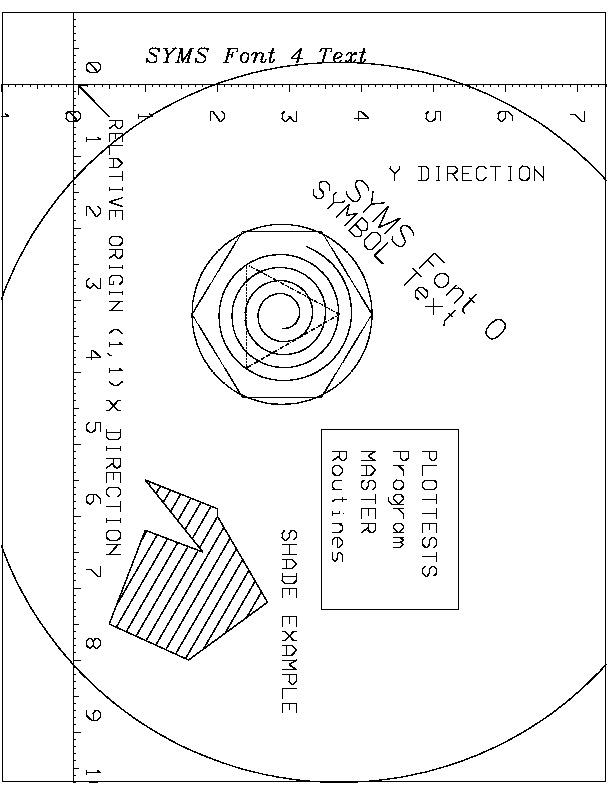
\includegraphics[width=3in,angle=90,origin=c]{figures/plottests0.jpg}\\
\vskip 40pt
{\large Version 8.0}\\
\today\\
\vskip40pt
Microwave Earth Remote Sensing Research Group (MERS)\\
Electrical and Computer Engineering Department \\
Brigham Young University\\
Provo, UT  \ \ \ 84602\\
\end{center}
\newpage
%\addcontents{toc}{chapter}{Table of Contents}
\tableofcontents

\begin{abstract}
\index{abstract}
The LONGLIB library is a set of subroutines originally written in
DEC VAX/VMS FORTRAN that has been updated to support other fortran dialects
including gfortran. The code has been translated into archaic but workable C.
The package is designed to create line graphics, but has some support for
pixel images. The package supports three classes of graphics devices:
(1) terminals that support graphics such as Xterm and Tektronics,
(2) printers and hardcopy devices via an intermediate meta files, and
(3) pixel-based displays such as an X window or a standalone monitor (RamTek).

A general set of graphics commands provides information simultaneously to
one or more of these output classes. The line graphics commands are based
on moving a virtual pen on the surface, e.g., a "pen up" move to a position
on a virtual sheet of paper, then a "pen down" move to a series of other
positions that draws a line, followed by a "pen up" or "new pen" to change
the color/width/line-type of the pen. The positions are specified in user
units which are converted to scalled output positions for the particular
output class.  For terminals, escaped text strings are sent to switch the
display to graphics mode and then draw lines, followed by a switch back to
terminal text mode. For printers, the commands recorded in a "meta" file
which is later processed by a meta converter to generate an output file for
the particular hardcopy device desired, e.g., postcript. A "replot" program
plots the contents of the meta file to a terminal or pixel-based display.
For pixel-based displays, the pen movements are either sent directly to
the display drawing code (e.g., the X windows interface) or converted to
pixel address in an array that are set to the specified color. The array
can output to a file or display on a display (e.g., X-windows or an archaic
display monitor originally termed a "Ramtek" display in the code).

High level routines that provide pen movement comments are provided that
draw character and number strings, as well as provide finished plots with
axes in 2 or 3 dimensions.

The archaic nature of the code and its operation are acknowledged, but it
has a number of unique advantages. It self-contained and requires no other
libraries, other than optionally linking to X windows. It includes routines
that can draw directly into pixel arrays. This include characters. The code
is free and pieces from the library can be adapted for other uses.

Longlib was originally written by an employee of a US government contractor and is in the public domain.

\end{abstract}

\chapter{Introduction}


\section{General}

This manual was prepared to document the most recent LONGLIB graphics
library.

The LONGLIB graphics library is a set of FORTRAN subroutines for
vector plotting (line graphics).  The library is similar to the
archaic CALCOMP or PLOT10 libraries; however, a great many extensions
are incorporated into the LONGLIB library including viewport clipping,
plot rotation, etc. In addition, the LONGLIB library includes a large
set of routines for such things as 3-d plotting (with hidden line
removal), extended character sets, MASTER routines, graphics input
routines, map routines, etc.


\section{Internal Packages}
\index{LONGLIB}\index{internal packages}\index{packages}
The LONGLIB library is designed with three internal packages for
plotting on 3 major classes of output graphics devices: graphics
terminals, display screens and/or windows, and hardcopy devices via
metafiles.  The packages are termed: 1) the Terminal Package, 2) the
RAMTEK Package, and 3) the Metafile Package.  Several options for the
RAMTEK Package are available including dummy routines, Ramtek display
screeen, X-Windows, and screen emulations.  A large variety of
graphics terminals, graphics terminal emulations, and hardcopy devices
are supported through the Terminal and Metafile Packages.

Graphics output to each type of device via the packages is discussed
below.  LONGLIB achieves virtual output device independence by using
only a minimum of low-level commands.  These include: initialization,
a clear/new page command, drawing vectors, line colors, line textures
(if supported on the selected graphics device), line widths (if
supported), and limited image capability for the screen/window devices
and the meta files.  Hardcopy devices which require rasterization are
also supported using the Metafile.

The library is principally designed for vector (i.e., line plotting)
with limited support for pixel graphics.  Lines are drawn by
specifying the movement of a virtual ``electronic pen".  The color,
width, and pattern of up/down motions in a line (the line type) may be
specified.  Capability for pixel-based graphics is provided for the
Ramtek screen/window package.  Images may be also be output to the
metafile.

The library consists of various subroutines which, when called by a
user-written program, produce line drawings on the desired
graphics device(s).  The system is interactive in the sense that the
user can see and modify plots immediately (on screen devices).  The
library can also produce a \x{metafile} which can then be processed by
programs supplied with the LONGLIB library to produce hardcopy output
on a variety of hardcopy devices.  Provisions have been incorporated
for device-dependent graphics input to a program (see \x{CURSOR}
routines).

The library is designed with several levels of graphics routine users
in mind.  For the user who simply wants to obtain a plot of an array
of data with a minimum of effort, the \x{MASTER} routines offer a
simple solution.  These routines handle opening/closing the plot
package, scaling, and axis generation, etc, a wide variety of formats.
For the user interested in more elaborate plots, access to several
levels of the plotting routines are provided.
\index{line type}
\index{color}

The LONGLIB graphics library supports both line type (such as pen
width and dot-dash patterns) and color attributes.  In general, these
attributes are device dependent and specific line types or colors used
on one plotting device may appear differently on a second device.
Typically, line width is simulated for graphics terminals while line
typing relies on hardware support.

Support for device-dependent image "maps" is also included (see
METMAP, RAMMAP, TEKMAP).

\section{Machine Dependence}
\index{machine dependent}

LONGLIB was developed in a \x{VAX/VMS} environment and was originally
written in FORTRAN.  However, it has also been ported to C.  The
system has been successfully ported to UNIX and LINUX systems on
various other machines including HP's, SUNs, Convex, intel, etc.

\subsection{FORTRAN}
While some machine-specific routines have been retained, the present
FORTRAN version of the library has been made as \x{FORTRAN-77}
compatible as practical.  Where the code is not FORTRAN-77 compatible,
it is so noted in the source code.  Most exceptions were made for
efficiency's sake and can be easily be modified or be left out of the
final library.

The largest FORTRAN-77 incompatibilities occur in the Ramtek packages
which can be left out of the library (see notes below).  Note that
some routine and common block names exceed the 6 character standard of
FORTRAN-77.  The auxilary, MASTER, and 3d plotting routines are
FORTRAN-77 compatible with a few minor exceptions (e.g. \x{INTEGER*2}
is used to save space) These exceptions are noted in the source code
file headers.  Source code contains tabs (control-I) and trailing
comments (separated by exclamation points (!).  The program \x{NOTABS}
(which is FORTRAN-77 compatible when a line is commented out) is
designed to remove tabs and trailing comments.

Routines in \x{RAMLIB}, \x{REFLIB}, and \x{CURSORLIB} are very machine
specific and may require extensive modification for use on other
machines.  A file NORAMLIB.FOR replaces all RAMLIB subroutines to
produce a no-Ramtek version of the library.

Unless specificially stated, integers are all assumed to be the
standard default machine length.  On most machines this is INTEGER*4.
A 2's complement representation is assumed for negative integers when
specifying the line type bit pattern (various routines and programs)
and in storing the pen motion data in the routines SYMBOL, SYM3D, and
SYM3DH.  The \x{cursor} routines CURMOTION, CURRECT, CURBAND use the
machine dependent routine \x{INXTCHR} to read escape sequences from
the terminal.  Note, however, that the library can be used without
these cursor routines.
\index{INTEGER*4}
\index{byte}

The \x{VAX} extended \x{FORTRAN} data type "BYTE" (for an 8 bit
variable) is used in the REF and Ramtek library package.
\index{\%loc()}
\index{\%val()}

\subsection{C}

The C language port was made with the assistance of F2C followed by
manual editing.  The C code consists of a mixture of ANSII C and
traditional C.  It has been successfully compiled and run using VAX C,
GNU C, HP C, and GNU C.  Most routines are available in both C
and FORTRAN, with the C versions the most up-to-date.

The documentation is primarily for the FORTRAN version of the
software.  For the C version:

\begin{enumerate}
\item All parameters are passed by reference (address).
\item All routine names end with an underbar, e.g., the routine
CALL PLOT(x,y,i) is called as plot\_(\&x,\&y,\&i).
\item FORTRAN CHARACTER variables are replaced with C strings.
\item FORTRAN BYTE or INTEGER*1 variables are replaced with C char
variables.
\end{enumerate}

An include ``my.h'' is used to specify the type ``integer'' as an
``int''.


\section{Modifying LONGLIB to Support Additional Graphics Devices}

When modifying LONGLIB to support additional graphics devices, one of
two approaches can be used.  One approach is to add an additional
terminal graphics device option.  The second approach is to add an
option to the RAMTEK package.  This is particularily appropriate for
devices which support image mode.  In either case, the key file which
must be modified is longlib/ which contains all of the terminal
dependent code and a portion of the RAMTEK code.  For the second
approach, RAMLIB.FOR (and possibly REFLIB.FOR) must also need to be
modified.

\section{Using Longlib with Graphics Terminals: The Terminal Package}

One of three internal, separate packages used by LONGLIB is the
terminal screen graphics package.
The LONGLIB graphics library supports a variety of graphics \x{terminal} 
devices which use \x{Tektronix} graphics formats including:
\index{Selanar}
\index{vt100}
\index{vt125}\index{4105}\index{4014}\index{4105}\index{4107}
\index{vt240}\index{xterm}

\begin{enumerate}
\item VT100 equipped with a Selanar Corp. GR100 or GR100+
\item VT125 (VT100 + retrographics)
\item VT240 and compatibles
\item VT220 equipped with a Selanar SG220
\item Tektronix 4010/4014 and compatibles
\item Tektronix 4107/4109 and compatibles
\item PC and Mac Terminal emulation software
\item Graphon GO-235
\item Xterm program (under X-Windows)
\end{enumerate}

\index{PLOTVT}
\index{vtplot}
\index{newvpen}
\index{newvcol}
Other graphics terminals can be used by appropriate modification of the
terminal driver routines (CTERM, VTPLOT, NEWVPEN, NEWVCOL).  The routines
\x{FRAME} and \x{VPLOTS} also need to be modified. 
Escape sequences need for terminal initialization and mode switching
are handled in the subroutine CTERM.  When plotting is not done to the
terminal \x{CTERM} and other terminal specific routines are dummy
calls.  Note: plotting to the terminal is done by accumulating a set
of connected line segments created by \x{PLOT} or PLOTVT.  The line
segments are output to \x{terminal} only when the buffer length of 32
is exceeded or a "pen up" occurs.  Consequently, a "pen up" should be
issued to force all stored plot segments to be output to the terminal
prior to viewing screen, e.g., PLOT(0.,0.,5).

It is assumed that all terminals are configured in a standard fashion.
Because of the wide variety of terminal types, the specific settings
are not be given in this document.

In designing the terminal driver routines, the design philosophy has
been to take advantage of the capability that many graphics terminals
have to display both text and graphics independently on the screen.
That is, the text and graphics "screens" can be independently cleared,
etc.  This feature is heavily exploited in this library.  Of course
not all terminals support this feature.  Terminals such as the VT240
and Tektronix 4010's do not support this feature.  In this case,
the \x{CTERM} routine operates somewhat differently in that it sets
the terminal to graphics mode and leaves it there.

Note that in the VAX environment, the SET TERM options of the terminal
driver must be properly configured.  For example, you must execute a
SET TERM/FORM while in \x{DCL} to enable the screen clear command to
work properly.  This permits a form feed to pass through to the
terminal.  The NO ESCAPE qualifier should also be set to read from the
terminal.

LONGLIB also supports color on graphics terminals which permit color
plotting (Tektronics 410x).

\subsection{Terminal Specific Application Notes}

The following sections describe the operation of the LONGLIB graphics
routines with some specific graphics terminal types.  This list is
not comprehensive.

\subsubsection{VT100 (w/Selanar Graphics Cards)}

A reference to a VT100 indicates a VT100 equipped with a Selanar
equipped (GR100, or GR100+) VT100.  A SG100 equipped VT100 has three
modes: the terminal (VT100) mode, the Selanar terminal mode, and the
Selanar graphics mode.  The routine \x{CTERM} is used to switch the
terminal between modes.  A call to \x{FRAME} sets the mode to the
Selanar terminal mode.  Whenever a line is plotted to the screen the
mode is changed to Selanar graphics and then back to the Selanar
terminal mode.  If a program error occurs when the terminal is in the
Selanar graphics mode, it is possible that no output appears.
Running the \x{CLEAR} command file resets the device back to
terminal mode.  The Selanar card does not provide linetypes or XOR
capability in the 4010 operation mode.

\subsubsection{VT125}

A \x{VT100} upgraded with the DEC upgrade package to a VT125 has two
modes used by the LONGLIB library: the normal terminal mode, and the
Tektronix 4010 graphics mode.  Both text and graphics can be displayed
on the same screen but independently manipulated by switching between
modes.  Running the \x{TCLEAR} command file resets the mode back
to terminal.

\subsubsection{VT240}

Unlike other terminals, the \x{VT240} when switched between terminal modes
clears the screen.  Thus CTERM sets the terminal mode to the Tektronix
4010 mode when terminal graphics are initiated.  The mode is not changed.
A limited set of linetypes is supported, though XOR plot mode is not.

\subsubsection{VT220 (w/Selanar Graphics Card)}

Reference to a \x{VT220} terminal is intended to indicate a VT220
terminal equipped with a Selanar SG220 graphics upgrade board.  The
SG220 board operates through the VT220's printer port.  In addition,
it uses some of the keys on the VT220 keyboard.  It is possible to
enable the graphics board when the printer port is disabled.  This
causes some of the keys (notably the keypad and cursor keys) to not
work for editing, etc.  To correct this, deselect the graphics board
using CNTRL-SELECT.

In order for the graphics board to plot graphics commands from the
library routines, the printer port must be in the controller mode and
the board enabled.  All this is automatically handled by the LONGLIB
graphics library routines.  Note, however, that you need to use
the CTERM commands correctly to obtain proper operation.

The command file \x{VCLEAR.com} resets printer port, reset the
graphics card to terminal mode, and clear the screen under most
situations.
\index{getcursor}

When using GETCURSOR, a large cross-hair appears on the screen.
Use the cursor keys and the shift key to move the intersection point to
the desired location and press a key.  This ends the graphics input.
The cross-hair disappears, there is a pause, and the program
continues.  NOTE: DON'T USE THE RETURN KEY TO END GRAPHICS INPUT AS
THIS CAUSES THE PROGRAM TO NOT READ THE LOCATION AND MESSES UP YOUR
TYPE-AHEAD BUFFER.

The SG220 board stores the starting and ending points of each vector
in memory then dynamically redraws the screen for each refresh (this
is how it can do zooming and windowing).  However, this also limits
the number of vectors that can be drawn on the screen at once.  If a
very large number of vectors are plotted, a zoom in/out may cause a
portion of them to not reappear.

Note:  Since the actual SG220 screen resolution is only 832x350
and the board is emulating a Tektronix 4014 (4096x3200) there is some
quantization error associated with the cross-hair operation.

Note: When the manual zoom in/out feature is used the cross-hair
cursor does not work properly.  The cross-hair is initially plotted
then erased.  When you move the cross-hair, it is replotted.  A copy
of the cross-hair stays at the start location.  Otherwise, it is
useable.

\subsubsection{Tektronix 4010/4014 Compatible Terminals}
\index{4010}
\index{4014}

A generic \x{Tektronix} 4010/4014 compatible terminal is defined in
LONGLIB.  Linetypes are supported.  Since most \x{Tektronix} 4010/4014
compatible terminals do not support dual text/graphics screens, this
feature is unavailable. 

\subsubsection{Tektronix 4105/4107/4109 Compatible Terminals}
\index{4105}
\index{4107}
\index{4109}

The \x{Tektronix} 410x terminals support a dual (text and graphics)
screen mode which is exploited by LONGLIB.  Most of the advanced
features available on these terminals are not exploited.  Color and
linetypes are supported.  The command file \x{ACLEAR} (executed from
DCL) can be used to clear the screen and reset the terminal into the
ANSI mode.

\subsubsection{Graphon Terminals}

The \x{Graphon} GO-235 is a terminal compatible with a VT100/VT200 and
Tektronix 4014.  It permits both text and graphics on the same screen
in separate planes when properly configured.  This configuration is
assumed by the LONGLIB graphics library.  The Graphon terminal supports
linetypes, graphics input, and XOR plot mode.
A command file GCLEAR (executed
from DCL) is provided to clear the screen and reset to text mode.

\subsubsection{Xterm program}
\index{Xterm}
Support for the X-Windows program Xterm is provided through \x{Tektronix}
4010/4014 codes and control codes to switch between a text terminal
emulation screen (VT100) and a graphics Tektronics emulation screen.
Linetypes are supported.


\section{The LONGLIB Metafile (Hardcopy Output) Package}

The second internal package used by LONGLIB is the \x{metafile} or
printer history file package.  The library can optionally produce a
plot metafile containing scaled, clipped pen motion commands.  This
"history" file can be processed by other programs to produce hardcopy
output on the appropriate device.  Using the \x{REPLOT} program, the
plot history file can be redisplayed on a screen device.  Raster scan
converter programs produce a dot-image printable file from the
metafile for printing to a dot matrix printer.  Other metafile
processing programs convert the LONGLIB metafile to other graphics
description languages including POSTSCRIPT, HPGL, QUIC, etc.
\index{postscript}
\index{hpgl}
\index{quic}
\index{stripping}
\index{strips}

Many of the LONGLIB metafile processing programs permit ``striping" of
the graphics image.  When the graphics image contained in the LONGLIB
metafile exceeds the size of a single page (or whatever) of the output
device, the the metafile image is ``cut" into "strips" which fit on
the output page.  Then each page is output.  Normally, blank pages are
suppressed.  At the same time redundant pen motions, changes, etc. are
filtered out.

\subsection{Dot Matrix Printers}
\index{raster scan}
\index{dot matrix printers}

Dot matrix printers, in general, require graphics data in a bit-mapped
image format.  This requires converting the LONGLIB metafile pen
motion file into a bit-image file using a raster scan process.
Using one of the supplied raster scan converter programs, the LONGLIB
metafile can be processed to produce a printable file of graphics for
several types of dot matrix printers.  The raster scan converter programs
supports linetypes and widths.  Currently, raster scan
converter programs which include "stripping" exist for the following
printers:

\begin{enumerate}
\item Printronix (PRNTRX)
\item Trilog TIP-300 (TRILGLO or TRILGHI--see below)
\item DEC LA50 (or compatible) (LA50)
\item Postscript
\item Encapulated Postscript
\end{enumerate}

The raster scan converter programs using ``stripping" with a strip
size which depends on the printer.  Ordinarily the strip is 56.5 by
13.2 inches (or the width of the printer page).
To generate a raster scan data file suitable for printing on a
dot matrix printer from the vector plot command file, the
raster scan converter program must be used.

Two raster scan programs have been provided for the
\x{Trilog} printer to take advantage of its higher printing resolution.
\x{TRILGLO} prints the same resolution on the Trilog printer as on the
Printronix printer.  \x{TRILGHI} plots at almost twice the
across-the-page resolution and the same down-the-page resolution.
Execution time is longer for the high resolution program.
\index{raster scan conversion}

An example of the use of the TRILGLO program in the \x{VAX} environment
follows.  The LONGLIB metafile input is FOR003.DAT.  The output
is OUT.LIS.
\begin{verbatim}

     $ TRILGLO :== $LONGLOC:TRILGLO
     $ TRILGLO FOR003.dat            ! run raster scan converter
     $ print/que=Trilog OUT.LIS      ! print output

\end{verbatim}

\x{VAX} \x{DCL} command files in the directory pointed to by the logical name
LONGLOC: contain command files for execution of these commands.
(PLOT183.COM = printronix printer, PLOTLO.COM = trilog printer lo-res
PLOTHI.COM = trilog printer hi-res).

\subsection{HPGL Compatible Pen Plotter}
\index{pen plotter}

Metafile conversion programs which convert the LONGLIB metafile into
an HPGL (\x{Hewlett-Packard} Graphics Language) command data file
are included in LONGLIB.  Three programs are available, HPGL, HPGL2,
and HPGLS.

\x{HPGL} reads the LONGLIB metafile, processes it into appropriate commands and
sends the commands to the terminal printer port (either a VT100 or
VT220 compatible terminal or a VT100 equipped with a Selanar GR100
graphics board) to which is connected an HPGL-compatible pen plotter.
No ``stripping" of the image is done.  The user is prompted for page
changes.  Pen changes on the plotter occur in response to a color
change in the metafile.  Line types are supported but line widths are
ignored.

\x{HPGL2} reads the LONGLIB metafile and produces a separate output file of HPGL
commands for each page of LONGLIB metafile input.  HPGL2 does not
include "stripping" of the image.  HPGL2 plots all of the vectors of a
given color before changing
pens.  Line types are supported but line widths are ignored.

\x{HPGLS} is similar to HPGL2 but includes stripping of the image.
HPGL2 produces a separate output file of HPGL commands for each strip
and page of LONGLIB metafile input.

An example of the use of the HPGL2 program in the \x{VAX} environment
follows.  The LONGLIB metafile input is FOR003.DAT\footnote{The standard C
language name is ``3.dat''.  The metafiles produced by the FORTRAN
libraries and the C libraries are NOT compatible.}.  The output
is a file, OUT.LIS which can then be sent to an HPGL-compatible plotter.
\begin{verbatim}

     $ HPGL2 :== $LONGLOC:HPGL2
     $ HPGL2 FOR003.dat            ! run HPGL conversion program
                                   ! several out.lis files may be produced
     $ print/que=HPGL out.lis;*    ! send output file(s) to plotter
\end{verbatim}

\subsection{QMS QUIC Laser Printer}

Three programs, LASER, LASERS, and RLASER, are included to convert the
LONGLIB metafile into a printable file in the \x{QMS} \x{QUIC} laser
printer control language.  Line width and line types are supported
though color is not.  Programs LASERS and RLASER "strip" the metafile
into 8.5 by 11 page strips while LASER does not do stripping.
\x{LASER} and \x{LASERS} produce a full size, normal orientation
output, while \x{RLASER} scales the output by 3/4 and rotates the
page -90 deg.

An example of the use of the LASER program in the \x{VAX} environment
follows.  The LONGLIB metafile input is FOR003.DAT.  The output
is OUT.LIS.
\begin{verbatim}

     $ QMS :== $LONGLOC:LASER
     $ QMS FOR003.dat               ! run QMS metafile conversion
     $ print/que=QMSLASER OUT.LIS   ! print output to printer
\end{verbatim}

\subsection{PostScript}

A program titled \x{POSTSCRIPT} is included which converts the
LONGLIB metafile into a PostScript page language format.  This can
then be printed to PostScript compatible printer (such as an Apple
Laserwriter).  No ``strips" are used. Linetypes and width are
supported.  Input color changes are output as gray tones.  \x{METMAP}
output is supported with 256 \x{gray} "levels" (0=black, 255=white).
The postscript converter supports image mode output with a maximum
size of 256x256 pixels per ``image''.

An example of the use of the POSTSCRIPT program in the \x{VAX}
environment follows.  The LONGLIB metafile input is FOR003.DAT.  The
output is OUT.LIS.
\begin{verbatim}

     $ POST :== $LONGLOC:POSTSCRIPT
     $ POST FOR003.dat                ! run POSTSCRIPT conversion
     $ print/que=POSTSCRIPT OUT.LIS   ! print output to printer
\end{verbatim}


\subsection{Plotting the LONGLIB Metafile to a Screen Device}

The program \x{REPLOT} has been provided which reads the
LONGLIB \x{metafile} created by an eariler program and plot the file
to a screen device (terminal or Ramtek).

\section{The RAMTEK Package}
\index{ramtek emulation}
\index{ref}

The third internal package (which is not available in some
installations) used by LONGLIB is the \x{Ramtek} Screen display
package.  Several options are available including the Ramtek family of
displays, X windows, and a Ramtek Emulation File (REF) package which
simulates a bit-mapped Ramtek display screen.  Unlike the Terminal
Package, the RAMTEK Package assumes that the display device is NOT
coupled to the text input/output so that screen clears, etc., do not
affect the user's text.  In addition, RAMTEK Package devices are
pixel-mapped and generally include color.

The RAMTEK Package options are available on different versions of the
Longlib libraries.\index{X Windows} The LONGLIB library can be
configured without any of the Ramtek package options using
the \x{NORAMLIB} file.

The Ramtek package is initialized by a call to \x{FRAME} (which calls
RPLOTS).  When the Ramtek package is not being used, calls to Ramtek
routines are dummy calls.  Note: plotting to the Ramtek is done by
accumulating a sequence of connected line segments (defined
by \x{PLOT} or PLOTRM) in a storage buffer.  The line segments are
output to the \x{Ramtek} only when the buffer length of 128 is
exceeded or a ``pen up" occurs.  Consequently, a final ``pen up"
should be issued to make sure all plot segments are output to the
display prior to viewing screen.

The Ramtek supports line types and scale factors as well as color and
line widths.

\subsection{X Windows Display Option}

Virtually all of the functions available on other RAMTEK Package
options are available for the X Windows Option.  This option has been
ported to X11R5 as well as
DecWindows. \index{X11R5}\index{DecWindows}\index{X Windows}

When the Ramtek package device is initialized, a X window is created
with one of several possible standard sizes or a custom size window
may be created.  Using low-level library calls, the user may also open
additional windows in which the rest of the LONGLIB routines may plot.
Note that, as of this writing, a specific process for refreshing the
windows has not been written.  Thus, refresh events can only occur
when a Ramtek routine is currently running.  This can lead to delays
in refreshing the window when an expose event occurs.  An event loop
routine which may be called by the user has been provided.

Routines have been included which permit writing image mode data in
either byte, integer*2, or integer*4 word sizes to the window.  Button
and key press events can be captured.


\subsection{Ramtek Emulation File Option}
\index{ramtek emulation file}
\index{REF}

When a Ramtek display is not available or to permit off-line plotting
to a "simulated" Ramtek device, a set of routines known as
the \x{Ramtek} Emulation File (REF) routines are included in LONGLIB.
These routines replace the Ramtek communications routines (RAMLIB) in
a version of the LONGLIB graphics library named LONGLIBR.OLB.  This
software emulates many (but not all) of the important functions of the
Ramtek communication routines to a 9460 or 9050 Ramtek display using
an internal byte array.  The \x{REF} subpackage uses some \x{VAX}
FORTRAN specific constructs (for efficiency) but could easily be
modified for


\subsubsection{Using the REF Routines}
\index{RMWRITEWORD}\index{REF}\index{Ramtek}\index{BYTE}\index{color table}

To use the REF routines, link to the LONGLIBR version of the LONGLIB
library, and plot to the Ramtek device.  The REF routines use a BYTE
array as the simulated Ramtek display.  The maximum size of the array
is 1600x1024.  The size used depends on the ``device'' or window size
selected during the package initialization.  Each byte of the array
stores the color table index for each pixel of the simulated Ramtek
display.  An empty "screen" consists of all zeros.  When a line is
drawn to the display using \x{PLOT} or \x{PLOTRM} the appropriate
pixel bytes are set to the line color.  REF routines also permit image
mode writing/reading of horizontal or vertical lines of bytes (see
RMWRITEWORD, for example).  When the plot package is closed (by a call
to PLOTND) the user is prompted to output the internal BYTE array
to a specific device (a graphics terminal, a metafile, or a special
REF file).  To avoid the interative prompt, the user can
call \x{REFDIS} (with its appropriate arguments) prior to
the \x{PLOTND} call.  This disables the prompts.  See REFDIS for
additional details.

Note: the Ramtek color table routines and cursor routines are dummy
calls when using the REF routine library.

\subsubsection{REF File Output}

\index{REF}
The REF file consists of a direct access file with a record length of
one horizontal line of pixels.  The number of records and record size
depends on the type of Ramtek chosen\footnote{For the C language
version, two short ints preceed the first line which give the size
(x,y) of the array.  In fortran, the record and file lengths are used
to determine the array size of the file.}  REFDIS places each
horizontal line of the output array into each record of the REF file.
The REF file can subsequently be read by the \x{REFTERM} program and
plotted to the "real" Ramtek device.  To produce a hardcopy output of
the REF file on a \x{QMS} laser printer, the program \x{REFLAS} reads
the file and produces a simulated gray scale image with 4 gray levels.
REFLAS prompts the user for the appropriate inputs.  In
the \x{VAX/VMS} environment, the program \x{REFLAS2} can be used.
REFLAS2 provides significantly faster run times by using the VAX
paging utility and downloadable fonts.

\subsubsection{REF Terminal or Metafile Output}

When outputing the byte array data to a terminal or printer history
file, the array is converted to a series of horizontal vectors.  As
the array scanned left to right, top to bottom, all ajacent pixels of
the same color are combined into a single vector.  When a pixel of a
different color is encountered the vector is output.  Pixels of color
"0" (background) are not output.  See REFDIS for additional details.


\subsection{Ramtek Display Option}

Currently, only some (but not all) of the functions of the Ramtek 9460
(1280x1024) or 9050 (512x512) Ramtek screen display are supported.
The current version of the software drivers for the Ramtek display are
machine specific to VAX/VMS.  This Option is available only in FORTRAN.
\index{vax/vms}

\x{Ramtek} display drivers expect the logical name "RM" be assigned to Ramtek
device (example: assign RMA0: RM:).  When the Ramtek device supports
multiple diplays, interaction between the displays complicates
matters.  To distiguish between different displays on the same device
it is suggested that the 0th device be named xxx0:, second device
xxx1:, etc. \x{Color} plotting is done on the Ramtek using the
previously loaded color table. The LONGLIB "color" is the color table
index.  The default Ramtek color table index is 255.  The main LONGLIB
package uses only vector plotting.  However, auxilary routines have
been included which permit writing image mode data to the Ramtek (or
REF) and for color table manipulation (see RMWRITEWORD or RMWRITECOL).
\index{RMWRITEWORD}
\index{RMWRITECOL}


\section{Disclaimer}

LONGLIB is powerful stand-alone graphics package for line-graphics.
Originally written in fortran in the mid-1980s, and translated to C in
the early 1990's, it is old but still useful algorithms and
code. Howeve LONGLIB was developed in the \x{VAX} \x{VMS} environment.
With the possible exception of the Ramtek package routines, the code
remains compatible with FORTRAN-77 but can be used with modern fortran
implementations such as gfortran on linux systems.  No claim is made
regarding the transportability other systems.  As with any software
system, there are the documentation or software and the documentation
is out of date.

\chapter{Programming Examples}

In this chapter several \x{examples} of using some of the basic plotting
routines of this library are included.  Other examples are in the
examples subdirectory. 
Examples for both \x{FORTRAN} and \x{C} routines are shown.

\section{FORTRAN Programming Examples}

For the user interested in obtaining very simple plots of curves
without being concerned with the details of LONGLIB, the \x{MASTER}
routines provide the most simple approach.  Greater control of the
output plot can be obtained by customizing user version of MASTER-like
routines from the auxilary routines.

\subsection{Simple MASTER Routine Example}

A very simple example of using the \x{MASTER} routines of this library
is shown below.  For more detailed examples see the following
sections.

This example plots a damped sine wave on both the terminal screen, the
Ramtek (in color), and the LONGLIB metafile.  The master
routine \x{PLOTSC} handles all graphics intialization and closing.
(See the chapter on MASTER routines for additional details).

\begin{verbatim}

           DIMENSION X(100),Y(100)
           DATA P,U,PL,A,B,PHI/112,85,25.,.013,.3/
           DATA PI/3.141593/
C  FILL DATA ARRAYS
           DO 10 I=1,100
             X(I)=I-1
             Y(I)=SIN((I-1)*PI/A+PHI)*EXP(-I*B)
     10    CONTINUE
C CALL LONGLIB PLOTTING ROUTINE TO PLOT CURVE.
C OUTPUT ONLY 35 OF THE 100 POINTS ON A 6X5 PLOT WITH TITLE
C AND A GRID.  iflag IS SET TO PROMPT FOR A SCREEN OUTPUT DEVICE.
C NOTE THAT WHEN A MASTER ROUTINE INITIALIZES LONGLIB, A
C METAFILE IS ALWAYS PRODUCED.
           CALL PLOTSC(X,Y,100,5,6.,5.,'X TITLE',7,'Y TITLE',7,
         1        'TOP TITLE',-10)
           STOP
           END

\end{verbatim}

\subsection{Lower Level Routines}

An example of using the auxilary routines of LONGLIB library from
\x{FORTRAN} is illustrated below.
An example for using this library from \x{C} follows.

This example plots a damped sine wave on both the terminal screen,
the Ramtek (in color), and the LONGLIB metafile.  No MASTER
routines are used.
\begin{verbatim}

       PROGRAM DEMO
       DIMENSION X(100),Y(100),ICOL(3)
       DATA P,U,A,B,PHI/112,85,25.,.013,.3/
C ICOL IS THE COLOR ARRAY FOR AXES
       DATA PI/3.141593/,ICOL/1,2,3,4/
C FILL DATA ARRAYS WITH Y=F(X)
       DO 10 I=1,100
         X(I)=I-1
         Y(I)=SIN((I-1)*PI/A+PHI)*EXP(-I*B)
   10  CONTINUE
C INITIALIZE LONGLIB WITH SCREEN PROMPT OPTION
C AND CREATE METAFILE TO FORTRAN UNIT 3.
       CALL FRAME(3,0,2.,2.,1.)
C COMPUTE SCALING FACTORS FOR X AND Y
       CALL SCALE(X,8.,100,1,1,XMIN,DX)
       CALL SCALE(Y,6.,100,1,1,YMIN,DY)
       Y0=-YMIN/DY
C PLOT COORDINATE AXISES WITH COLOR OPTION ENABLED
       CALL AXIS(0.,Y0,'X-AXIS',-6-100000,20.,0.,
      1  XMIN,DX,N1,N2,ICOL)
       CALL AXIS(0.,0.,'SINE',4+100000,17.,90.,
      1  YMIN,DY,N1,N2,ICOL)
C SET LINE COLOR
       CALL PLOT(5.,0.,0)
C PLOT DATA POINTS AS A LINE WITH SYMBOLS
       CALL LINE(X,Y,100,1,5,2,1,1,XMIN,DX,YMIN,DY)
C PICK UP PEN AT END OF LINE (FORCES OUTPUT TO SCREENS)
       CALL PLOT(0.,0.,3)
C PROMPT FOR SCREEN CLEAR ON RAMTEK/TERMINAL
       CALL CTERM(2)
       CALL RTERM(2)
C CLOSE LONGLIB
       CALL PLOTND
       STOP
       END
\end{verbatim}

\section{C Language Programming Example}
\index{c language}
The following is an illustration of how to use lower level LONGLIB
routines to produce a plot from \x{VAX} C.

\begin{verbatim}

/* Example in VAX C */

main 
{
  real x[100],y[100],dx,xmin,dy,ymin;
  real exp(),sin(),y0;
  int icol[4] = 1 , 2, 3, 4;
  int i,n1,n2;
  real pi = 3.141592654;
  real p = 112., u = 85., a = 25., b = .013, phi = .3;

  for (i = 1; i < 100 ; i++) {
    x[i] = i - 1;
    y[i] = sin( (i-1) * pi / a + phi) * exp(-i * b);
  }
  frame_(&3,&-3,&0.,&0.,&1.);          /* Initialize */
  scale_(x,&8.,&100,&1,&1,&xmin,&dx);
  scale_(y,&6.,&100,&1,&1,&ymin,&dy);
  y0 = -ymin / dy;
  plot_(&2.,&2.,&-3);                  /* new origin */
  axis_(&0.,&y0,"X-AXIS",&-6-100000,&20.,&0.,&xmin,&dx,&n1,&n2,icol);
  axis_(&0.,&0.,"SINE",&4+100000,&17.,&90.&ymin,&dy,&n1,&n2,icol);
  plot_(&4.,&0.,&0);                   /* new color */
  line_(x,y,&100,&1,&5,&2,&1,&1,&xmin,&dx,&ymin,&dy);
  plot_(&0.,3&0.,&3)                   /* pen up */
  cterm_(&2);                          /* ask if screen clear */
  plotnd_();                           /* terminate plotting */

}
\end{verbatim}

\section{MASTER Routine Examples (FORTRAN)}

The subsections that follow illustrate additional examples of how to use
MASTER routines from FORTAN.

\subsection{Adding Additional Annotation to a MASTER Routine Plot}
\index{PLOTSC}
\index{plottests}

The following is an \x{example} of using a MASTER
subroutine more than once and/or adding additional text or
another plotting line and/or two MASTER subroutines: (see also the
program PLOTTESTS)


\begin{verbatim}
       ...
C INCLUDE PLOTSC ROUTINE COMMON BLOCK WHICH RETURNS
C SCALE FACTORS USED IN PLOTTING
       COMMON /CPLOTSC/XMR,DXR,YMR,DYR 
       ...
C CALL PLOTSC WITH -10000 iflag < 0 TO INITIALIZE LONGLIB
C BEFORE CALL BUT NOT CLOSE LONGLIB AFTER CALL
C SET iflag TO PROMPT FOR SCREEN DEVICE TYPE WITH TICKED GRID
       CALL PLOTSC(X,Y,25,4,8.,6.,'X AXIS',6,
     1    'Y AXIS',6,'TITLE',-5,ICOL)
C PUT GRAPHICS TERMINAL IN GRAPHICS MODE
       CALL CTERM(-1)
C PLOT ADDITIONAL TEXT AFTER PLOT TITLE
       CALL SYMBOL(999.,999.,0.15,' TEXT',0.,5,-1)
C PLOT ADDITIONAL ANNOTATION ABOVE PLOT
       CALL SYMBOL(0.0,6.5,0.15,'NUMBER=',0.,7,-1)
C ADD NUMBER AFTER ANNOTATION WITH 3 DIGITS AFTER DECIMAL PT.
       CALL NUMBER(999.0,999.0,0.15,3.1415,0.,0.3,-1)
C CHANGE LINE TYPE TO DOTTED
       CALL NEWPEN(1)
C ADD ANOTHER LINE OF DATA ON PLOT USING PLOTSC SCALE FACTORS
       CALL LINE(X,Y2,N,1,0,0,1,1,XMR,DXR,YMR,DYR)
       ...
C ASK IF SCREEN CLEAR ON TERMINAL (METAFILE NOT AFFECTED)
       CALL CTERM(2)
       CALL PLOTND
       ...
\end{verbatim}

\subsection{Using Multiple MASTER Routines in the Same Program}
\index{plottests}

The following is an \x{example} of how to use several MASTER
subroutines in the same program.  (see also the program PLOTTESTS)
The basic idea is to use the first call to a MASTER routine to
initialize the LONGLIB graphics library.  On later calls to MASTER
routines you must use "iflag" to instruct the routine NOT to
re-initialize LONGLIB.  The last call to a MASTER routine closes
LONGLIB.
\index{PLOTLG}
\index{PLOTSC}


\begin{verbatim}
C FIRST CALL TO MASTER ROUTINE, SET -10000 < iflag < 0
C TO INITIALIZE LONGLIB BUT NOT CLOSE IT
C SET iflag TO PROMPT FOR SCREEN DEVICE TYPE WITH
C AXIS ON TOP AND SIDES AND NO GRID
       CALL PLOTSC(X,Y,N,-1,...) 
       ...
C SECOND CALL TO MASTER ROUTINE, SET iflag < -10000 TO
C PREVENT INITIALIZING LONGLIB OR CLOSING IT
C SET iflag TO PRODUCE AXIS TICKED GRID (SINCE
C LONGLIB OPEN, NO PROMPT FOR SCREEN DEVICE)
       CALL PLOTSC(X,Y,N,-10004,...)
       ...
C LAST CALL TO MASTER ROUTINE, SET iflag > 10000 TO
C PREVENT INITIALIZING LONGLIB AND CLOSE IT AFTER PLOTTING
C SET iflag TO PRODUCE AXIS TICKED GRID AND LOG/LOG FORM
C (SINCE LONGLIB OPEN, NO PROMPT FOR SCREEN DEVICE)
       CALL PLOTLG(X,Y,N,10053,...)
\end{verbatim}

\subsection{MASTER Routine Color Example}
\index{PLOTSC}

The following is a very elaborate example of how to use color in a particular
MASTER routine (PLOTSC).


\begin{verbatim}
C DIMENSION AND LOAD COLOR ARRAY
       DIMENSION ICOL(6)
       DATA ICOL/1,2,3,4,5,6/
       ...
C CALL PLOTSC WITH NUMBER OF TITLE CHARACTERS NEGATIVE TO
C USE COLOR ARRAY.  SET iflag TO INITIALIZE/CLOSE LONGLIB
C SET iflag TO PRODUCE AXIS TICKED GRID
        CALL PLOTSC(X,Y,25,4,8.,6.,'X AXIS',6,
     1    'Y AXIS',6,'TITLE',-5,ICOL)
       ...
\end{verbatim}

\newpage
\subsection{Using Multiple MASTER Plots on Same Page/Screen}
\index{PLOTSC}

The following is a very elaborate example of how to to place several
MASTER routine plots on the same Ramtek and terminal screen but different
metafile pages.


\begin{verbatim}
C OPEN LONGLIB OUTSIDE OF MASTER ROUTINE
C SELECT BOTH TERMINAL AND RAMTEK SCREEN OUTPUT WITH NO
C SCREEN CLEAR ON RAMTEK OR TERMINAL
       CALL FRAME(3,-3,1.,1.,1.)
C CHANGE COLOR AND ADD A SEPARATE PLOT TITLE
       CALL PLOT(7.,0.,0)
       CALL SYMBOL(6.,11.5,.3,'TITLE',0.,5,-1)
C CHANGE ORIGIN AND SHRINK SUBSEQUENT PLOTS ON RAMTEK/TERMINAL
C BUT NOT METAFILE
       CALL PLOT(1.,1.,-3)
       CALL VFACTOR(.5)
       CALL RFACTOR(.5)
C LOOP TO PLOT FOUR MASTER PLOTS ON ONE SCREEN
       DO 10 I=1,4
C CALL PLOTSC WITH iflag < 10000 TO NOT INITIALIZE
C LONGLIB OR CLOSE IT AFTER PLOT
C SET iflag TO PRODUCE AXIS TICKED GRID 
C (SINCE LONGLIB OPEN, NO PROMPT FOR SCREEN DEVICE)
        CALL PLOTSC(X,Y,25,-10004,8.,6.,'X AXIS',6,
     1    'Y AXIS',6,'TITLE',5)
C MOVE ONLY RAMTEK AND TERMINAL ORIGINS BUT NOT METAFILE
        CALL PLOTRM(0.,2.*5.,-3)
        CALL PLOTVT(0.,2.*5.,-3)
        IF (I.EQ.2) CALL PLOTRM(11.,-20.,-3)
        IF (I.EQ.2) CALL PLOTVT(11.,-20.,-3)
C NEWPAGE ON METAFILE (DOES NOT AFFECT TERMINAL/RAMTEK)
        CALL NEWPAGE
10     CONTINUE
       ...
C PROMPT FOR SCREEN CLEAR ON RAMTEK/TERMINAL
       CALL CTERM(2)
       CALL RTERM(2)
C CLOSE LONGLIB
       CALL PLOTND
       ...
\end{verbatim}


\chapter{Description of Plotting Routines}

This chapter details the central LONGLIB graphics library routines.
A brief description of each routine is shown along with an example
of its call and a description of the associated parameters.
Parameters are shown in <> brackets are optional in systems permitting
optional parameters.  They are are not accessed unless specifically
requested by other parameters values\footnote{In C, all parameters are
passed by reference (address).  FORTRAN CHRACTER data types are replaced
with C char.  BYTE types are replaced with char.}.

The name of each parameter is followed by a letter indicating
the variable type.  Unless otherwise specified, integers are the
default integer length of the machine (which is \x{INTEGER*4} on the VAX).
\index{byte}
\index{integer}
\index{real}
\index{character}
\index{logical}
\begin{verbatim}

     I = INTEGER 
     R = REAL
     C = CHARACTER 
     L = LOGICAL

\end{verbatim}

Lengths are given in the standard plot units of inches.  The routine
\x{FACTOR} can be used to change the plot unit length.  Angles are specified
in degrees counter-clockwise from the x axis.

Unless specifically noted all parameters passed into a routine via the
call statement are used as ``read-only", i.e., they are
not be modified by the routine.

\section{SUBROUTINE ARROW}

\x{ARROW} plots a vector arrow at any desired point and with any desired
angle.  The type of arrowhead drawn may be selected.
\begin{verbatim}

CALL ARROW (x,y,al,a,p,b)

x,y  (R): location coordinates for vector-arrow tail
al   (R): length of arrow in plot units
          if al=0, only a single point at (x,y) is output
a    (R): angle from horizontal at which the arrow is to be drawn
          (deg counterclockwise)
p    (R): length of arrowhead in plot units
          > 0 open arrowhead    ( --> )
          = 0 no arrowhead
          < 0 closed arrowhead  ( -|> )
b    (R): angle between arrowhead side and arrow line (deg)
\end{verbatim}

\section{SUBROUTINE AXIS}

\x{AXIS} plots a single coordinate axis with numeric labels at any desired 
location and angle.  The routine has to be
called separately for the x and y axis.  A possible exponent
is determined and placed at the end of the axis title in the form
of 10**n.  In  order  to  leave room  for the labelling the
axis should be removed at least by 3/4 inch from the edge of the plotter page.
The length of the axis should be integer-valued.  The (i)th (i=0 to ml-1)
axis major tick is labeled with the value, xm+dx*i.
For a log axis see LGAXS.
\begin{verbatim}

CALL AXIS (x,y,s,n,al,a,xm,dx<,nm,ml<,ic>>)

x,y  (R): location of starting point of the axis
s    (C): character variable containing the axis title
n    (I): number of characters in the string s
          > 0 : axis labelling on positive side (anti-clockwise)
          < 0 : axis labelling on negative side (clockwise)
 (100's digit)    = 0 : coordinate line, ticks and labels drawn
                  = 1 : line and ticks only--no labeling
 (1000's digit)   = 0 : numeric labels paralel to axis line
                  = 1 : numeric labels orthogonal to axis line
 (10000's digit)  = 0 : additional optional parameters ignored
                  = 1 : additional optional parameters used
 (100000's digit) = 0 : color list ignored
                  = 1 : color list used
al   (R): length of axis in plot units (real number, integer-valued)
          > 0 : tick marks placed on same side of axis as title
          = 0 : no action (return with no plotting)
          < 0 : tick marks placed on opposite side of axis from title
a    (R): angle at which the coordinate axis is to be drawn
xm   (R): value of first marking on the axis
dx   (R): increment for numeric axis labels
(NOTE: the following parameters are accessed only if the
       magnitude of n is > 10000)
mn   (I): minor tick marks between labeled major ticks
           if not specified, 0 is used
ml   (I): number of labeled major tick marks
           if not specified, int(l) is used
ic   (I): array of color values, if color not enabled,
           current color is unchanged
          ic(1) : color value for axis line and ticks
          ic(2) : color value for numbers on axis
          ic(3) : color value for axis label 
                  (color upon return if no exponent plotted)
          ic(4) : color for auto exponent scale
                  (color upon return if exponent shown)
\end{verbatim}

\section{SUBROUTINE AXIS2}

\x{AXIS2} is similar to AXIS but allows additional flexibility to draw
different tick sizes and types.  Optionally, a possible exponent
is determined and placed at the end of the axis title in the form
of 10**n.  In  order  to  leave room  for the labelling the
axis should be removed at least by 3/4 inch from the edge of the plotter page.
The length of the axis should be integer-valued.  The (i)th (i=0 to ml-1)
axis major tick is labeled with the value, xm+dx*i.
AXIS2 plots a coordinate axis and its markings at any desired location 
and angle.  For a log axis see LGAXS.
\begin{verbatim}

CALL AXIS2 (x,y,s,n,al,a,xm,dx<,nm,nn,ml,ts,nd,sm<,ic>>)

x,y  (R): location of starting point of the axis
s    (C): character variable containing the axis title
n    (I): number of characters in the string
          > 0 : axis labelling on positive side (anti-clockwise)
          < 0 : axis labelling on negative side (clockwise)
 (100's digit)    = 0 : coordinate line, ticks and labels drawn
                  = 1 : line and ticks only--no labeling
 (1000's digit)   = 0 : numeric labels paralel to axis line
                  = 1 : numeric labels orthogonal to axis line
 (10000's digit)  = 0 : optional parameters ignored
                  = 1 : optional parameters used
 (100000's digit) = 0 : color list ignored
                  = 1 : color list used
al   (R): length of axis in plot units (real number, integer-valued)
          > 0 : tick marks placed on same side of axis as title
          = 0 : no action (return with no plotting)
          < 0 : tick marks placed on opposite side of axis from title
a    (R): angle at which the axis is to be drawn
xm   (R): value of first marking on the axis
dx   (R): increment for the axis markings
(NOTE: the following paramters are accessed only if the
       magnitude of n is > 10000)
nm   (I): number of minor tick marks between major ticks,
           if not specified, 0 is used
nn   (I): nn-th minor tick is high-lited in length, if
           not specified, 0 is used (none)
ml   (I): number of labeled major tick marks, if not specified
           then one major tick per inch is used
          < 0 use following additional parameters used
          > 0 use following additional parameters ignored
(NOTE: the following paramters are accessed only if the
       magnitude of n is > 10000 and ml < 0)
ts   (R): character size of title and numbers, if not
           specified, 0.15 is used
          > 0 auto exponent scaling (x10 to power) is enabled
          < 0 auto exponent scaling (x10 to power) disabled
nd   (I): number of digits to right of decimal point, if not
          specified 1 is used
sm   (R): major tick length, if not specified 0.1 is used
          note that minor tick length is 1/2 major tick length
ic   (I): array of color indexes for axis colors
          ic(1) : color value for axis line and ticks
          ic(2) : color value for numbers on axis
          ic(3) : color value for axis label 
                  (color upon return if no exponent plotted)
          ic(4) : color for auto exponent scale
                  (color upon return if exponent shown)
\end{verbatim}

\section{SUBROUTINE AXIS3}

\x{AXIS3} plots a single axis and its markings at any desired location and
angle.  Optionally, a possible exponent
is determined and placed at the end of the axis title in the form
of 10**n.  The length of the axis can take any value.  The (i)th (i=0 to ml-1)
axis major tick is labeled with the value, xm+i*(xx-xm)/le.
This version of axis is more flexible than other versions
and permits specifying the axis number labeling format.
For a log axis see LGAXS.
\begin{verbatim}

CALL AXIS3 (x,y,s,n,al,a,xm,xx,t,c,f,ic)

x,y  (R): starting location of the axis
s    (C): character variable containing the axis title
n    (I): number of characters in the string
          > 0 : axis labelling on positive side (anti-clockwise)
          < 0 : axis labelling on negative side (clockwise)
 (100's digit)    = 0 : coordinate line, ticks and labels drawn
                  = 1 : line and ticks only--no labeling
 (1000's digit)   = 0 : numeric labels paralel to axis line
                  = 1 : numeric labels orthogonal to axis line
 (100000's digit) = 0 : color list ignored
                  = 1 : color list used
al   (R): length of axis 
          > 0 : tick marks placed on same side of axis as title
          = 0 : no action
          < 0 : tick marks placed on opposite side of axis from title
a    (R): angle at which the axis is to be drawn 
xm   (R): value of first marking on the axis
xx   (R): value of last marking on the axis
t    (R): number of tick marks 
          specification is coded in the form MMM.mmss where
          MMM is the number of major tick marks ( MMM > 0), mm is
          the number of minor tick marks between major tick marks
          (100 > mm => 0), and ss is the number of subminor tick
          marks between minor tick marks (100 > ss => 0).
          (example 1.0102 produces I_._._i_._._I)
c    (R): size of characters 
          < 0 auto exponent scaling (x10 to power) disabled
          > 0 auto exponent scaling (x10 to power) enabled
f    (R): axis number label format (see NUMBER)
ic   (I): array of color indexes for axis colors
          ic(1) : color value for axis line and ticks
                  (color upon return if no labels)
          ic(2) : color value for numbers on axis
          ic(3) : color value for axis label 
                  (color upon return if no exponent plotted)
          ic(4) : color for auto exponent scale
                  (color upon return if exponent shown)
\end{verbatim}

\section{SUBROUTINE CIRCLE}
\index{PLTARC}
\index{arc}

\x{CIRCLE} plots circles, arcs and spirals.  The curve is approximated by small
straight line segments.  The radius of the curve determines the number of line
segments used.  See also PLTARC. A solid circle of radius 2.0 centered at the
origin could be generated by the call,
\begin{verbatim}

CALL CIRCLE(0.0,0.0,0.0,360.0,2.0,2.0,0.0).

\end{verbatim}
Note that the hardware line type in effect before the call to circle
would be used to draw the circle.  A dashed-line (software generated)
spiral centered at (1,1) would be created by the call,
\begin{verbatim}

CALL CIRCLE(1.0,1.0,90.0,800.0,3.0,1.0,0.5).
\end{verbatim}
\begin{verbatim}

CALL CIRCLE (x,y,aa,ao,ra,ro,d)

x,y  (R): coordinates for the center of the circle
aa   (R): angle in degrees of starting point of curve
ao   (R): angle of end point relative to start point
ra   (R): curve radius at starting point
ro   (R): curve radius at the end point
d    (R): =  0 : solid curve
          = .5 : dashed curve (software generated dashes)
\end{verbatim}


\section{SUBROUTINE CSHADE}

The \x{CSHADE} subroutine fills in an \x{area} defined by a segment of a \x{circl}e
using equally spaced lines at a given angle with a 
specified line type.  A full circle may be used.
\begin{verbatim}

CALL CSHADE (x,y,r,a1,a2,s,l,d,t,w,m1,m2)

x,y   (R): location of circle center
r     (R): segment or circle radius
a1,a2 (R): segment start and stop angles (a2>=a1)
            if a2-a1=360 a full circle is used otherwise
            the area is a pie segment
l     (I): shade format control
           = -3 : clear area and outline
           = -2 : clear area
           = -1 : clear outline
           =  0 : no action
           =  1 : draw outline
           =  2 : shade area
           =  3 : shade area and outline
d     (R): distance between shading lines
t     (R): angle of shading lines in degrees
w     (R): working array dimensioned at least 3*n where
            n=int((a2-a1)/(180*atan(s/r)/pi)+1)
m1    (R): line type of shading
            < 0 : shading done with current line type
           => 0 : new line type (see NEWPEN)
m2    (R): line type for area outline
            < 0 : use prior line type
           => 0 : new line type (see NEWPEN)
\end{verbatim}

\section{SUBROUTINE CTERM}

\x{CTERM} is the central subroutine for controling the state of the graphics
terminal.  It is used to switch a graphics terminal
in and out of the graphics and text modes. It is a dummy call when not in
\x{terminal} plotting mode.  Note that not all options are available on all
terminals.  Results of operation of this routine is thus terminal dependent.
In some cases the graphics and text modes are the same while in others,
the mode is switched only at init/de-init.
See the introduction to the documentation under terminal types.  See also
\index{ICTERM}.

\index{FRAME}
Note:  for CTERM(2), the user is prompted for a "clear screen".
The reply may be "Y" for yes, "N" for no (the default), "Q" (quit), 
"S" (skip one), "P" (pass many), or "D" (dump).  "Y" and "N" clear
the screen as indicated and the program continues normally.
A reply of "Q" permanently disables terminal screen plotting until
the package is reinitialized by FRAME.  A replot of "S" disables
screen plotting until the next CTERM(2) call whereupon the 
"clear screen" prompt reappears as before.  A reply of "P" is similar
to "S", but the user is prompted for the number of \xx{CTERM}(2) calls
to pass before reissuing the prompt.  In this manner multiple terminal
screen "pages" can be skipped.  A reply of "D" enables a dump
of the screen to the attached terminal printer (if supported on the
particular terminal/printer).  Note that during a skip that any changes
of origin by PLOT, scale factors by \x{FACTOR} or VFACTOR, or pen color
or linetype does NOT take place.
\begin{verbatim}

CALL CTERM (iarg)

iarg (I): terminal operation code
          = 0 : initialize graphics mode on terminal
          = 1 : return terminal from graphics to text mode
          =-1 : return terminal text to graphics mode
          = 2 : return terminal to text mode, and prompt
                user for clear screen (see note above)
          =-2 : return terminal to text mode, clear graphics screen
          = 3 : clear text screen, leave in text mode
          =-3 : clear graphics screen, leave in terminal mode
          = 4 : dump graphics screen to printer
          =-4 : clear text, graphics, leave in graphics mode
          = 5 : turn off graphics screen, return to text mode
          =-5 : turn on graphics screen, return to graphics mode
          = 6 : toggle reverse video
          = 8 : de-initialize graphics terminal
\end{verbatim}

\section{SUBROUTINE DASHL }

\index{software line type}
\index{line type}
\x{DASHL} plots a software-generated dashed  \x{line} through the coordinate points
stored in x and y.  See also LINE.
\begin{verbatim}

CALL DASHL (x,y,n,k,j,l,ix,iy,xm,dx,ym,dy)

Parameter list description same as LINE.

x     (R): array containing the x coordinates
y     (R): array containing the y coordinates
n     (I): number of data points in x and y
           (the number of data points in x, y should be equal)
k     (I): plot every first (k=1), second (k=2) value etc
           (normally k=1)
j     (I): plotting symbol spacing flag
           > 0 : symbol is plotted at every jth plotted point
                 connected by lines
           = 0 : no symbols, lines only
           < 0 : symbol is plotted at every abs(j)th plotted point
                 with no connecting lines
l     (I): plot symbol number (see SYMBOL)
ix,iy (I): starting indexs in array (normally ix,iy=1)
xm    (R): minimum value scale factor for x array
dx    (R): increment scale factors for x array
ym    (R): minimum value scale factor for y array
dy    (R): increment scale factors for y array
\end{verbatim}

\section{SUBROUTINE ELLIPSE}

\x{ELLIPSE} plots all or part of a parametric ellipse of the form,
\begin{verbatim}

        (x,y) = (maj*cos(t), min*sin(t))

\end{verbatim}
where maj and min are the major and minor ellipse axes, respectively
and where t is the parametric angle specification.  Part of the ellipse
can be plotted by specifying only part of the range of t.
The major axis center line is offset by the angle am.
The angles ast and aend define the starting and ending
angles for t.  Note that aend should be greater than ast.
The ellipse is approximated by short, straight line segments.  The number
and length of the segments depend on the size of the ellipse.
\begin{verbatim}

CALL ELLIPSE (x,y,maj,min,am,ast,aend)

x,y  (R): center of ellipse (halfway between foci)
maj  (R): length of semi-major axis (distance between center and
          curve through one focus)
min  (R): length of minor axis (distance between center and
          curve perpendicular to semi-major axis)
am   (R): angle of semi-major axis from horizontal
          (deg counter-clockwise)
ast  (R): start angle of curve from semi-major axis
          (deg counter-clockwise)
aend (R): end angle of curve from semi-major axis
          (deg counter-clockwise) note: aend > ast
\end{verbatim}

\section{SUBROUTINE FACTOR}

Positional information is usually expressed in inches.  A conversion \x{factor}
can be given for other units, such as "cm". The new coordinate values are
derived from the product "fac*x" where x is the input value.
A negative value or zero resets the
scaling factor to unity.  Note that the initial factor can be specified
in FRAME.  The subroutine \x{FACTOR} calls PFACTOR, RFACTOR, and VFACTOR which
change the scale factors for the metafile, Ramtek, and terminal
packages, respectively.  These routines can be called separately to 
affect only the scale factor of the particular package.
\index{FRAME}
\index{PFACTOR}
\index{RFACTOR}
\index{VFACTOR}
\begin{verbatim}

CALL FACTOR (fac)

fac (R): new conversion factor for coordinate values (all packages)
         <= 0 : scale factor reset to unity
         >  0 : new scale factor
\end{verbatim}

\section{SUBROUTINE FRAME}

\index{Selanar}
\index{vt100}
\index{vt125}
\index{vt240}
\index{vt220}
\index{Tektronix 4010/4014}
\index{Tektronix 4107/4109}
\index{Xterm}
\x{FRAME} initializes the graphics metafile/terminal/Ramtek software  and
resets internal  variables.  This routine is usually the first LONGLIB
routine called (also see \x{PLOTS} which calls FRAME).  FRAME must be activated
before plotting calls are issued by the user program.  FRAME should
normally be called only once in a program.  MASTER routines optionally
handle the FRAME call.

FRAME intializes the graphics output device packages.  The FORTRAN
unit number used for the LONGLIB metafile can be specified.  Normally,
unit 3 is used.  If unit 0 is specified, FRAME prompts the user
for a yes/no response to create a metafile.  A negative unit number
disables the metafile package.  All calls to metafile routines (such
as PPLOT) are dummy calls when the metafile package is disabled.

FRAME also initializes the screen graphics device.  A screen device
code is used to determine whether the Ramtek or Terminal screen device
packages are open.  If a negative value for the screen device code
is used the screen device is not cleared prior to use, otherwise it is.
If the screen device code is +/- 4, no screen device package is used and
all calls to screen
specific routines (such as PLOTRM or PLOTVT) are dummy calls.
If a screen device code of 0 is used, the user is prompted for 
a screen device to use.  The screen devices may then be selected using
a character code.  A reply of "?" lists the available options.

\index{X-Axis}
\index{Y-Axis}
FRAME also intializes the origin and scale factor for plotting.
The default origin on the \x{terminal} and the \x{Ramtek} is the lower
left of screen (0.,0.).  The X axis runs horzontally, while the Y axis
runs vertically.  The default origin on the printer is the upper left
corner of page.  The X axis runs vertically down page, while the Y axis runs
horizontally across the page.

When the \x{Ramtek} Screen device is selected, FRAME opens a communications
channel to the Ramtek.  If no channel is available or the Ramtek is in use an
error message is typed and the calling program is terminated.
\begin{verbatim}

CALL FRAME (pl,id,vpx,vpy,zom)

pl   (I): Fortran file unit number (normally 3) used for LONGLIB
          Metafile.  If pl < 0 then no metafile is generated.
          If pl = 0 then the user will be prompted for a yes/no
          metafile.  In this case unit number used will be 3.
id   (I): Screen device code number.
          < 0 : Do not clear Ramtek/terminal screens prior to use.
          > 0 : Clear Ramtek/terminal screens prior to use.
          = 0 : Prompts user for which screen device to use.
                A ? response will list the available devices.
          = 1 : Use VT100 as Screen Output (only) (Selanar GR100)
          = 2 : Use Ramtek as Screen Output (only).
          = 3 : Use both Ramtek and VT100 as Screen Output.
          = 4 : Do not produce Screen output.
          = 5 : Use VT125 as Screen Output (only)
          = 6 : Use VT100 as Screen Output (only) (Selanar GR100)
          = 8 : Use VT240 as Screen Output (only)
          = 9 : Use VT220 as Screen Output (only) (Selanar SG220)
          =10 : Use Tektronix 4010/4014 as Screen Output
          =11 : Use Tektronix 4107/4109 as Screen Output
                (color Tektronix)
          =12 : Use Graph-On GO-235 as Screen Output
          =13 : Use Xterm (Tektronics with control codes)
vpx, (R): relative x,y offset of the bottom left hand corner of
vpy       the screen/page.  Equivalent to PLOT(vpx,vpy,-3).
zom  (R): The value of 'zom' scale factor. (see FACTOR)
\end{verbatim}

\section{SUBROUTINE GRID}
\index{LGRID}

\x{GRID} plots a \x{Cartesian} grid or solid lines or ticks at
grid intersections.  See also LGRID.
\begin{verbatim}

CALL GRID (x,y,dx,dy,nx,ny)

x,y   (R): coordinates in the bottom left corner of grid
dx,dy (R): spacing of grid lines in x and y directions
nx,ny (I): number of grids in x and y direction
           if nx > 0 and ny > 0 then solid grid plotted
           if nx < 0  or ny < 0 then tick grid plotted
           if nx < 0 and ny < 0 then boxed tick grid plotted
\end{verbatim}

\section{SUBROUTINE HISTON}

\x{HISTON} controls the output to the metafile.  The metafile MUST have been
previously initialized to re-enable output.
\begin{verbatim}

CALL HISTON (I)

l     (I): action flag
           = -1 : disable output to metafile
           = +1 : enable output to metafile

\end{verbatim}

\section{SUBROUTINE HLT3D}

\index{PLT3D}
\index{2-d surface plotting}
\x{HLT3D} plots a 2 dimensional array to produce a 2-d histogram similar
to PLT3D.  Hidden lines are supressed.
Transformation from the array indices (i,j) to (x,y,z) is:
\begin{verbatim}

    x = xl * .5 * float(2*j-n-1)/float(n-1)
    y = yl * .5 * float(2*i-m-1)/float(m-1)
    z = zs * (a(i,j) + z0)

Thus,

    (1,1) is (-xl/2,-yl/2)   (m,1) is (-xl/2,+yl/2)
    (1,n) is (+xl/2,-yl/2)   (m,n) is (+xl/2,+yl/2)

    xplotted = x*cos(az) - y*sin(az) + x0
    yplotted = x*sin(az)*sin(al) + y*sin(az)*sin(al) + z*cos(al) + y0
\end{verbatim}

The common block \x{PLT3B} returns these \x{transformation} parameters so
that the plotted location (xp,yp) of the corner of the cube corresponding
to the point (i,j,zr) may be computed as:
\begin{verbatim}

        xp = a1 * j + a2 * i + a3
        yp = b1 * j + b2 * i + b3 * zr + b4
\end{verbatim}

The dimension of the working array is dependent on the
surface complexity -- the greater the surface complexity, the greater
l2 must be.  As a minimum, l2 > 4*min(m,n).  See also \x{NXTVU} and PLT3D.
\index{PLT3D}
\begin{verbatim}

CALL HLT3D (a,md,nd,m,n,w,l,w2,l2,al,az,xl,x0,yl,y0,zs,z0,ierr)

a     (R): array of values to be plotted dimensioned a(md,nd)
md,nd (I): array dimensions
m,n   (I): size of data in array to be plotted
w     (R): dummy variable so that call is compatible with PLT3D
l     (I): dummy variable so that call is compatible with PLT3D
w2    (R): working storage array dimensioned w2(l2)
l2    (I): working storage array dimension (see note)
al    (R): viewing altitude angle (deg)
az    (R): viewing azimuth angle (deg)
xl,yl (R): length of unprojected axes in plot units
x0,y0 (R): plot origin in plot units
zs    (R): z coordinate scale factor
z0    (R): z coordinate offset
ierr  (I): (returned) error code
           = 0 : ok
           = 1 : l2 not large enough in NXTVU

COMMON /PLT3B/ a1,a2,a3,b1,b2,b3,b4
\end{verbatim}

\section{FUNCTION ICTERM}

\x{ICTERM} is essentially equivalent to \x{CTERM} but can return the
user response to the calling program.

Note:  as in CTERM(2), the user is prompted for a "clear screen"
when a call to ICTERM(2) is made.  However, additional user options
are available including "X" for exit to user program and "<control>Z" or EOF.
Other replies include "Y" for yes, "N" for no (the default), "Q" (quit), 
"S" (skip one), "P" (pass many), or "D" (dump).  "Y" and "N" clear
the screen as indicated and the program continues normally.
A reply of "Q" permanently disables terminal screen plotting until
the package is reinitialized by FRAME.  A replot of "S" disables
screen plotting until the next CTERM(2) or ICTERM(2) call whereupon the 
"clear screen" prompt reappears as before.  A reply of "P" is similar
to "S", but the user is prompted for the number of \xx{CTERM}(2) or
\x{ICTERM}(2) calls to pass before reissuing the prompt.  In this manner multiple terminal
screen "pages" can be skipped.  A reply of "D" enables a dump
of the screen to the attached terminal printer (if supported on the
particular terminal/printer).  Note that during a skip that any changes
of origin by PLOT, scale factors by \x{FACTOR} or VFACTOR, or pen color
or linetype does NOT take place.
\begin{verbatim}

iret = ICTERM (iarg)

iarg (I): terminal operation code
          = 0 : initialize graphics mode on terminal
          = 1 : return terminal from graphics to text mode
          =-1 : return terminal text to graphics mode
          = 2 : return terminal to text mode, and prompt
                user for clear screen (see note above)
          =-2 : return terminal to text mode, clear graphics screen
          = 3 : clear text screen, leave in text mode
          =-3 : clear graphics screen, leave in terminal mode
          = 4 : dump graphics screen to printer
          =-4 : clear text, graphics, leave in graphics mode
          = 5 : turn off graphics screen, return to text mode
          =-5 : turn on graphics screen, return to graphics mode
          = 6 : toggle reverse video
          = 8 : de-initialize graphics terminal
iret (I): (returned) user option code
          = 0 : normal user response (Y,N,S, etc.)
          = 1 : user exit (X) response
          =-1 : EOF or "^Z" response
\end{verbatim}

\section{SUBROUTINE  LGAXS}

\x{LGAXS} plots a single \x{logarithmic} coordinate \xx{axis}. Complete
decades are produced.  See also \x{AXIS} and LGLIN.
\index{LGLIN}
\begin{verbatim}

CALL LGAXS (x,y,s,n,al,a,nmin,dx<,ic>)

x,y   (R): location starting point of the axis
s     (C): axis label string
n     (I): number of characters in string
           > 0 :  label on positive side
           < 0 :  label on negative side
 (100's digit)   = 0 : coordinate line, ticks and labels drawn
                 = 1 : line and ticks only--no labeling
 (1000's digit)  = 0 : numeric labels paralel to axis line
                 = 1 : numeric labels orthogonal to axis line
 (10000's digit) = 0 : color list ignored
                 = 1 : color list used
al    (R): length of axis
           > 0 : axis ticks placed on same side of axis as title
           = 0 : no action (return with no plotting)
           < 0 : ticks placed on opposite side of axis from title
a     (R): angle at which the axis should be plotted
nmin  (R): number to be printed at the first axis tick (power of ten)
dx    (R): scaling factor in the form dx=(nmax-nmin)/l where
           nmax, nmin are the exponent powers at the start
           and end of the axis
ic    (I): color array (accessed if mag(n)>10000))
           ic(1) : color for axis line and ticks
           ic(2) : color for numbers
           ic(3) : color for axis title
\end{verbatim}

\section{SUBROUTINE LGLIN}
\index{LINE}

\x{LGLIN} plots a solid curve through a set of values from x to y.
Either x or y or both may in the process be converted to
\x{logarithmic} form.  Symbols may be used at selected intervals.
(see also \x{SCALG} and LINE).  The plotted x values are computed according to,
\begin{verbatim}

    for logarithmic scaling,

       xplotted= (alog10(abs(x(i))+1.e-38)-xm)/dx

    for linear scaling,

       xplotted= (x(i)-xm)/dx

\end{verbatim}
and similarily for y.
\begin{verbatim}

CALL LGLIN (x,y,n,k,j,l,lg,ix,iy,xm,dx,ym,dy)

x     (R): array containing the x coordinates
y     (R): array containing the y coordinates
n     (I): number of data points in x and y
           (the number of data points in x,y must be equal)
k     (I): take every first (k=1), second (k=2) value etc.
           (normally k=1)
j     (I): plotting symbol spacing flag
           > 0 : symbol is plotted at every jth plotted point
                 connected by lines
           = 0 : no symbols, lines only
           < 0 : symbol is plotted at every abs(j)th plotted point
                 with no connecting lines
l     (I): plot symbol number (see SYMBOL)
lg    (I): log option
           = - 2 : x and y are plotted using logarithmic scaling
           = - 1 : x logarithmic, y linear
           =   1 : x linear, y logarithmic
ix,iy (I): start index if arrays (normally ix,iy=1)
xm    (R): minimum value scale factor for x array
dx    (R): increment scale factors for x array
ym    (R): minimum value scale factor for y array
dy    (R): increment scale factors for y array
\end{verbatim}

\section{SUBROUTINE  LGRID}

\x{LGRID} plots a \x{logarithmic} or linear \x{grid} using solid lines,
dotted lines, or ticks.  See also GRID.
\begin{verbatim}

CALL LGRID (x,y,dx,dy,nx,ny,i)

x,y   (R): location coordinates for the bottom-left corner of grid
dx,dy (R): spacing of major grid lines in x and y directions
nx    (I): number of major grid lines in x direction
           < 0 : log spacing of minor lines
           > 0 : no minor lines/ticks
ny    (I): number of major grid lines in y direction
           < 0 : log spacing of minor lines
           > 0 : no minor lines/ticks
i     (I): option flag
           = 0 : solid major/minor lines
           = 1 : dotted major/minor lines
           = 2 : solid major lines with minor ticks
\end{verbatim}

\section{SUBROUTINE LINE}

\x{LINE} plots a solid curve through a set of coordinate pairs
stored in two arrays. Symbols may be inserted at selected
intervals and points of curves may be skipped.
The coordinates are calculated as follows:
\begin{verbatim}

        xplotted(i)=(x(i)-xm)/dx, i=ix to n, step k
        yplotted(m)=(y(m)-ym)/dy, m=iy to n, step k

\end{verbatim}
The routine \x{SCALE} may be used to compute the scale factors xm, dx,
ym, and dy from the x and y arrays.
\begin{verbatim}

CALL LINE (x,y,n,k,j,l,ix,iy,xm,dx,ym,dy)

x     (R): array containing the x coordinates
y     (R): array containing the y coordinates
n     (I): number of data points in x and y
           (the number of data points in x, y should be equal)
k     (I): plot every first (k=1), second (k=2) value etc
           (normally k=1)
j     (I): plotting symbol spacing flag
           > 0 : symbol is plotted at every jth plotted point
                 connected by lines
           = 0 : no symbols, lines only
           < 0 : symbol is plotted at every abs(j)th plotted point
                 with no connecting lines
l     (I): plot symbol number (see SYMBOL)
ix,iy (I): starting indexs in array (normally ix,iy=1)
xm    (R): minimum value scale factor for x array
dx    (R): increment scale factors for x array
ym    (R): minimum value scale factor for y array
dy    (R): increment scale factors for y array
\end{verbatim}

\section{SUBROUTINE LINE2}

\x{LINE2} is similar to line but, when connecting points, when
the distance between two x values is larger than ddx, does not
plot the connecting line.
\begin{verbatim}

CALL LINE2 (x,y,n,k,j,l,ix,iy,xm,dx,ym,dy,ddx)

x     (R): array containing the x coordinates
y     (R): array containing the y coordinates
n     (I): number of data points in x and y
           (the number of data points in x, y should be equal)
k     (I): plot every first (k=1), second (k=2) value etc
           (normally k=1)
j     (I): plotting symbol spacing flag
           > 0 : symbol is plotted at every jth plotted point
                 connected by lines
           = 0 : no symbols, lines only
           < 0 : symbol is plotted at every abs(j)th plotted point
                 with no connecting lines
l     (I): plot symbol number (see SYMBOL)
ix,iy (I): starting indexs in array (normally ix,iy=1)
xm    (R): minimum value scale factor for x array
dx    (R): increment scale factors for x array
ym    (R): minimum value scale factor for y array
dy    (R): increment scale factors for y array
ddx   (R): distance threshold for x
\end{verbatim}


\section{SUBROUTINE NEWPAGE}

\index{form feed}
\index{page}
\x{NEWPAGE} inserts a change page command into the LONGLIB metafile.  The
hardcopy conversion program use the change page command to issue a form
feed to the metafile output.  Note that NEWPAGE only affects the metafile page
and does not change origin, etc.
It is a dummy call for \x{Ramtek} or \x{terminal} plotting.  This command is
equivalent to CALL PLOT(0.,0.,10).
\begin{verbatim}

CALL NEWPAGE
      (no arguments)
\end{verbatim}

\section{SUBROUTINE NEWPEN}

\index{line type}
\index{ppen}
\index{rmpen}
\index{vpen}
\x{NEWPEN} calls PPEN, RMPEN, and VPEN which change the hardware line type
and/or width of the plotting line for subsequent plotting on the metafile,
Ramtek, and terminal output devices.  The precise effects depend on the
particular graphics device.  There are 9 standard line types which are 
shown in the last chapter.  The output device uses the nearest
hardware-supported line type to the standard line type.  Some
devices support additional types including permitting a specification
of the scale factor of the line type (the length of the dot/dash pattern).
If a device does not support line types, the default type is used.
Line widths are not support on the Ramtek packages and are simulated
in softwared for the terminal.  The metafile package supports all features
although the metafile processing programs may only use the
features supported by the particular hardcopy graphics output device.
Default line type is a solid line of width 1 dot.
\begin{verbatim}

CALL NEWPEN (i)

i  (I): selects a line type for all additional plotting
        for all output devices
        < 0 : resets line type to solid line of unit width.
        = 0 : no change
        > 0 : line type and width changed according to,
 (1's digit)   : line type (0-9) (value of 0 does not change type)
 (10's digit)  : line width (1-7) (value of 0 does not change width)
 (100's digit) : line type pattern scaling (1-7) (0 is no change)
\end{verbatim}

\section{SUBROUTINE NUMBER}

\x{NUMBER} plots a floating point number in a specified format using
a fortran format-like specification.  It also permits
free-format and exponential notation formats.  The number is converted
to an \x{ASCII} string plotted at a specified location and baseline angle
using SYMBOL.  The following table illustrates the dependence of the output
string on the type (integer/real) and value of the parameter e.  The table
shows the output for an input f=103.356 and i=-1.

\begin{verbatim}

         Output    integer e   real e
        --------   ---------- --------
         103          -1       1003.0
         103.          0        0.0
         103.          0        3.00
         x103.36                7.02
         103.36        2        0.02
         103.356000    6       10.06
         xx103                 1005.0
         **                    1002.0 (format overflow)
         x103.4                 6.01
         *.****                 6.04  (format overflow)
         .103E+02              -8.03
         *.***                 -5.03  (format overflow)

note: x=space, * indicates overflow
\end{verbatim}

\begin{verbatim}

CALL NUMBER (x,y,h,f,a,e,i)

x,y   (R): location position (x,y returned if i=-2 or -3)
           If x=999 then x is continued from lower right of
           prior call to SYMBOL or NUMBER.  If y=999 then
           y is continued.
h     (R): size (height) of digits
f     (R): floating point number to be plotted
a     (R): baseline angle at which to plot (normally zero)
e     (R): output format (e=n.j) 
           (similar to the FORTAN format statement Fn.j)
           n is the total number of characters (max 18) 
           including the decimal point and j is a two digit number
           specifying the number of digits to the right of 
           the decimal point (e.g., to get F6.4 use e=6.04)
             if e<0 number is plotted in exponential notation (En.j)
             if e=-1.0 then f is plotted free format exponential
             if e=1.0 then f is plotted free format real
             if e=0.0 then f is plotted as free format integer
             if n = 0 then f is plotted with j digits to
                      the right of the decimal point
             f will be plotted as a formatted m digit integer
               [i.e., (Im)] when e=1000+m.
i     (I): centering flag (see SYMBOL)
           = -3 : same as -2 but string is not plotted and
                  last position is not affected
           = -2 : same as -1 but returns end point in x,y
           = -1 : (x,y) is lower left corner of plotted array
           =  0 : (x,y) is center of plotted array
           =  1 : (x,y) is lower right corner of plotted array
           =  2 : no action
\end{verbatim}

\section{SUBROUTINE PFACTOR}

\x{PFACTOR} is called by \x{FACTOR} to change the input scale conversion factor
for the LONGLIB metafile package.  It may be called separately if desired.
Only the metafile plotting package
is affected.  The routines \x{RFACTOR} and \x{VFACTOR} may be separately 
called to change the input scale conversion factor on the Ramtek and
terminal packages, respectively.  See FACTOR.
\begin{verbatim}

CALL PFACTOR (fac)

fac (R): new conversion factor for coordinate values
         (only the metafile scaling is affected)
         <= 0 : scale factor reset to unity
         >  0 : new scale factor
\end{verbatim}

\section{SUBROUTINE PLOT}
\index{view port}
\index{origin}
\index{plotting window}
\index{PLOTRM}
\index{PPLOT}
\index{PLOTVT}

\x{PLOT} is the central routine for controlling the motion of the electronic
pen for all LONGLIB graphics device packages.  PLOT calls the Ramtek,
metafile and terminal PLOT routines PLOTRM, PPLOT, PLOTVT based on the
graphics devices initialized by FRAME.  These individual "package
PLOT" routines can be called separately if desired to affect only the
particular package.  Via these package-specific plot routines PLOT can
moves the pen, change the origin or pen color, issue a page change
command, etc.  A relative rotation angle for all successive plotting
may also be specified.  LONGLIB defines a plotting \x{window} or
viewport, the size of which is device dependent, within which pen
motions are clipped.  The viewport may be set to an arbitrary size
within the device plotting window (e.g. terminal screen).  An attempt
to make the viewport bigger than the device output forces the viewport
to be the device output window (this is the default).  For rotated
clipping regions see the \x{PLOTC} utility.

The transformation from an input point (x,y) in plot units to an output point
(nx,ny) in output device unit pixels (ignoring clipping, etc.) is:
\begin{verbatim}

    nx = (z * (x * cos( a ) - y * sin( a )) + ox) / rx
    ny = (z * (x * sin( a ) + y * cos( a )) + oy) / ry

where

    a is the relative plotting angle (expressed in radians)
    z is the zoom scale factor
    ox,oy is the scaled, rotated relative origin
    rx,ry is the screen resolution for each axis (inches/pixel)

\end{verbatim}
The relative plotting angle a is updated according to:
\begin{verbatim}

    anew = aold + ain

\end{verbatim}
and the relative origin (ox,oy) is updated according to:
\begin{verbatim}

    oxnew = z * (xin * cos( a ) - yin * sin( a )) + oxold
    oynew = z * (xin * sin( a ) + yin * cos( a )) + oyold
	
\end{verbatim}
\begin{verbatim}

CALL PLOT (x,y,i)

x,y   (R): coordinate values
i     (I): plot function parameter
           =  0: color control
                  x is the new line color
                  if x < 0 the screen is cleared
           =  2: draw to (x,y) with 'pen down'
           = -2: same as i=2. (x,y) becomes new origin
           =  3: move to (x,y) with 'pen up'
           = -3: same as i=3. (x,y) becomes new origin
           =  4: upper right corner of viewport set to (x,y)
           = -4: lower left corner of viewport set to (x,y)
           =  5: pick pen up at last point
           =  6: set relative plotting angle to x
           =  9: erase to (x,y) (plot with color 0)
           = -9: erase to (x,y) (x,y) becomes new origin
           = 10: issue change page command to metafile
           = 11: end plot (close LONGLIB)
           =999: end plot (close LONGLIB)
\end{verbatim}

\section{SUBROUTINE PLOTND}

\x{PLOTND} is used to signal LONGLIB that all plotting is complete.  It
sends the final output buffers to the respective graphics devices, closes
files and channels, and resets the terminal to the normal \x{text} mode.  PLOTND
is equivalent to a CALL PLOT(0.,0.,11) command.
\begin{verbatim}

CALL PLOTND
      (no arguments)
\end{verbatim}

\section{SUBROUTINE PLOTS}

\x{PLOTS} initializes the LONGLIB graphics package via a call to FRAME.
PLOTS provides compatibility with existing CALCOMP or PLOTS-10 compatible
code.  It simply calls \x{FRAME} with argurments which cause FRAME to prompt
for optional usage of the Longlib metafile output and a graphics
screen.  For new code use FRAME.
\begin{verbatim}

CALL PLOTS (...)

(arguments are ignored)
\end{verbatim}

\section{SUBROUTINE PLOTRM}

\x{PLOTRM} is the central routine for controlling the plotting of lines to
the Ramtek or REF package.  PLOTRM is called by the \x{PLOT} routine but
can be called separately.  Any call to PLOTRM when the Ramtek package
is not initialized is a dummy call.  Options for PLOTRM are similar
to PLOT (see documentation on PLOT).
An attempt to make the viewport bigger than the Ramtek screen window
forces the viewport to be the size of the Ramtek screen window
(this is the default).  Typically the Ramtek screen window is
either 13.75 or 11 by 11 inches depending on the type (1280x1024 and
512x512, respectively), with the lower
left corner at (0,0) and the upper right corner at (13.75,11).

The transformation from an input point (x,y) in plot units to an output point
(nx,ny) in pixels (ignoring clipping and any axis direction reversal) is:
\begin{verbatim}

    nx = (z * (x * cos( a ) - y * sin( a )) + ox) / rx
    nx = (z * (x * sin( a ) + y * cos( a )) + oy) / ry

where

    a is the relative plotting angle (expressed in radians)
    z is the zoom scale factor
    ox,oy is the scaled, rotated relative origin
    rx,ry is the screen resolution for each axis (inches/pixel)
(see WHERERM)
\end{verbatim}
\index{WHERERM}
The relative plotting angle a is updated according to:
\begin{verbatim}

    anew = aold + ain

\end{verbatim}
and the relative origin (ox,oy) is updated according to:
\begin{verbatim}

    oxnew = z * (xin * cos( a ) - yin * sin( a )) + oxold
    oynew = z * (xin * sin( a ) + yin * cos( a )) + oyold
	
\end{verbatim}
\begin{verbatim}

CALL PLOTRM (x,y,i)

x,y   (R): coordinate values
i     (I): plot function parameter
           =  0: Ramtek color control
                   x is the Ramtek color table index
                   if x < 0 the Ramtek screen is cleared
           =  2: Ramtek draw to (x,y) with 'pen down'
           = -2: same as i=2. point (x,y) becomes new origin
           =  3: Ramtek move to (x,y) with 'pen up'
           = -3: same as i=3. Point (x,y) becomes new origin
           =  4: upper right corner of viewport set to (x,y)
           = -4: lower left corner of viewport set to (x,y)
           =  5: pick pen up at last point
           =  6: set relative plotting angle to x
           =  9: draw to (x,y) 'pen down' color 0 (erase)
           = -9: same as i=9. Point (x,y) becomes new origin
           = 11: end plot (close Ramtek package)
           =999: end plot (close Ramtek package)
\end{verbatim}

\section{SUBROUTINE PLOTVT}

\x{PLOTVT} is the central routine for controlling the plotting of lines to
the terminal screen device REF package.  PLOTVT is called by
the \x{PLOT} routine but can be called separately.  Any call to PLOTVT
when the terminal package is not initialized is a dummy call.  Options
for PLOTVT are similar to PLOT (see documentation on PLOT).  An
attempt to make the viewport bigger than the terminal screen window
forces the viewport to be the size of the terminal screen window
(this is the default).  Typically the terminal screen window is 9.5 by
either 9.5 or 7.2 inches (depending on the terminal) with the lower
left corner at (0,0) and the upper right corner at (9.5,9.5).

The transformation from an input point (x,y) in plot units to an
output point (nx,ny) in pixels (ignoring clipping and any axis
direction reversal) is:
\begin{verbatim}

    nx = (z * (x * cos( a ) - y * sin( a )) + ox) / rx
    nx = (z * (x * sin( a ) + y * cos( a )) + oy) / ry

where

    a is the relative plotting angle (expressed in radians)
    z is the zoom scale factor
    ox,oy is the scaled, rotated relative origin
    rx,ry is the screen resolution for each axis (inches/pixel)
(see WHEREVT)
\end{verbatim}
\index{WHEREVT}
The relative plotting angle a is updated according to:
\begin{verbatim}

    anew = aold + ain

\end{verbatim}
and the relative origin (ox,oy) is updated according to:
\begin{verbatim}

    oxnew = z * (xin * cos( a ) - yin * sin( a )) + oxold
    oynew = z * (xin * sin( a ) + yin * cos( a )) + oyold
	
\end{verbatim}
\begin{verbatim}

CALL PLOTVT (x,y,i)

x,y   (R): coordinate values
i     (I): plot function parameter
           =  0: if x < 0 the terminal graphics screen is cleared
                 if x = 0 set terminal to erase mode plotting
                 if x <> 0 and x <> 999 set line color to x
                 if x = 999 set terminal to XOR mode plotting
                             (only if terminal has capability)
           =  2: draw to (x,y) with 'pen down' on terminal
           = -2: same as i=2. Point (x,y) becomes new origin
           =  3: move to (x,y) with 'pen up' on terminal
           = -3: same as i=3. Point (x,y) becomes new origin
           =  4: upper right corner of viewport set to (x,y)
           = -4: lower left corner of viewport set to (x,y)
           =  5: pick pen up at last point
           =  6: set relative plotting angle to x
           =  9: erase to (x,y) on terminal (if supported)
           = -9: same as i=9. Point (x,y) becomes new origin
           = 11: end plot (close terminal package)
           =999: end plot (close terminal package)
\end{verbatim}

\section{SUBROUTINE PLRAX}

\index{polar axis}
\x{PLRAX} plots a circular \x{axis} for plotting in polar form.  A series
of concentric circles are drawn around (x,y) at increasing radi
to the maximum radius.     Provisions are included for half circle,
quarter circle, etc.  Labeling of starting points and ending points
may be changed.
\begin{verbatim}

CALL PLRAX (x,y,r,as,ae,a0,a1)

x     (R): x coordinate of center of polar axis
y     (R): y coordinate of center of polar axis
r     (R): radius of polar axis in plot units
as    (R): starting angle of axis in degrees from horizontal
ae    (R): ending angle of axis in degrees from horizontal
           Note: as=0 and ae=360 yields full circle axis
a0    (R): number label of starting angle
a1    (R): number label of ending angle
           Note: if a0=a1 then angles are not labeled.
\end{verbatim}

\section{SUBROUTINE PLRLN}

\index{polar line}
\x{PLRLN} plots a solid curve through the set of coordinate points
in polar form stored in r and t arrays.  Symbols may be inserted
at selected intervals.     Angle values stored in the t array are
in degrees referenced to horizontal.  Coordinates are calculated
as follows:
\begin{verbatim}
          r=(r-rmin)/dr
          xplotted=r*cos(t*pi/180)
          yplotted=r*sin(t*pi/180)

\end{verbatim}
\begin{verbatim}

CALL PLRLN (r,t,n,j,l,ir,rmin,dr)

r     (R): array of radial values to be plotted
t     (R): array of angle values
n     (I): number of points to plot
j     (I): plotting symbol option flag
           > 0 : symbol plotted every jth point with connecting lines
           = 0 : line plotted only with no symbols
           < 0 : symbols plotted only, no connecting line
l     (I): symbol number (see SYMBOL)
ir    (I): start index in r and t arrays
rmin  (R): minimum radius scale factor
dr    (R): scale factor
\end{verbatim}

\section{SUBROUTINE PLTARC}
\index{circle}

\x{PLTARC} plots a circular \x{arc} segment through three specified points
using the routine CIRCLE.  The plotted arc starts at (x1,y1) and
pass through (x2,y2) before ending at (x3,y3).  In the event that any
two points are coincident or all three points are colinear, a line
segment from (x1,y1) to (x3,y3) is drawn.
\begin{verbatim}

CALL PLTARC (x1,y1,x2,y2,x3,y3)

x1    (R): x coordinate of first (start) point
y1    (R): y coordinate of first (second) point
x2    (R): x coordinate of second point
y2    (R): y coordinate of second point
x3    (R): x coordinate of last (end) point
y3    (R): y coordinate of last (end) point
\end{verbatim}

\section{SUBROUTINE PLT3D}

\index{2-d surface plotting}
\x{PLT3D} plots a 2 dimensional array as a surface scribed with a linear grid
parallel to the x and y axes, i.e., a mesh.  Hidden lines are supressed.
Transformation from the array indices (i,j) to (x,y,z) is:
\begin{verbatim}

    x = xl * .5 * float(2*j-n-1)/float(n-1)
    y = yl * .5 * float(2*i-m-1)/float(m-1)
    z = zs * (a(i,j) + z0)

Thus,

    (1,1) is (-xl/2,-yl/2)   (m,1) is (-xl/2,+yl/2)
    (1,n) is (+xl/2,-yl/2)   (m,n) is (+xl/2,+yl/2)

    xplotted = x*cos(az) - y*sin(az) + x0
    yplotted = x*sin(az)*sin(al) + y*sin(az)*sin(al) + z*cos(al)+y0
\end{verbatim}

The common block \x{PLT3B} returns these \x{transformation} parameters
so that the plotted location (xp,yp) of a point (i,j,zr) may be
computed as:
\begin{verbatim}

        xp = a1 * j + a2 * i + a3
        yp = b1 * j + b2 * i + b3 * zr + b4
\end{verbatim}

The dimension of the second set of working arrays is dependent on the
surface complexity -- the greater the surface complexity, the greater
l2 must be.  As a minimum, l2 > l.  See also \x{NXTVU} and HLT3D.
\index{HLT3D}
\begin{verbatim}

CALL PLT3D (a,md,nd,m,n,w,l,w2,l2,al,az,xl,x0,yl,y0,zs,z0,ierr)

a     (R): array of values to be plotted dimensioned a(md,nd)
md,nd (I): array dimensions
m,n   (I): size of data in array to be plotted
w     (R): working array dimensioned w(l) l=>4*min(m,n)
l     (I): working array dimension
w2    (R): working storage array dimensioned w2(l2)
l2    (I): working storage array dimension (see note)
al    (R): viewing altitude angle
az    (R): viewing azimuth angle
xl,yl (R): length of unprojected axes (plot units)
x0,y0 (R): plot origin
zs    (R): z coordinate scale factor
z0    (R): z coordinate offset
ierr  (I): (returned) error code
           = 0 : ok
           = 1 : l2 not large enough in NXTVU
           = 2 : l not large enough

COMMON /PLT3B/ a1,a2,a3,b1,b2,b3,b4
\end{verbatim}

\section{SUBROUTINE PPLOT}

\x{PPLOT} is the central routine for controlling the plotting of lines to
the LONGLIB metafile package.  PPLOT is called by the \x{PLOT} routine
but can be called separately.  Any call to PPLOT when the metafile
package is not initialized is a dummy call.  Options for PPLOT are
similar to PLOT (see documentation on PLOT).  An attempt to make the
viewport bigger than the metafile plotting window forces the
viewport to be the size of the metafile plotting window (this is the
default).  The metafile plotting window is 56.5 by 56.5 inches with
the lower left corner at (0,0) and the upper right corner at
(56.5,56.5).  Since most hardcopy devices can not produce such a large
output page, the LONGLIB metafile processor programs which convert the
metafile to an output file, "strips" the metafile window into
separate, overlapping output pages.  Only non-blank page strips are
output to the device.

The transformation from an input point (x,y) in plot units to an output point
(nx,ny) in metafile storage units (ignoring clipping) is:
\begin{verbatim}

    nx = (z * (x * cos( a ) - y * sin( a )) + ox) / rx
    nx = (z * (x * sin( a ) + y * cos( a )) + oy) / ry

where

    a is the relative plotting angle (expressed in radians)
    z is the zoom scale factor
    ox,oy is the scaled, rotated relative origin
    rx,ry is the metafile resolution for each axis (inches/res unit)
(see WHEREPR)
\end{verbatim}
\index{WHEREPR}
The relative plotting angle a is updated according to:
\begin{verbatim}

    anew = aold + ain

\end{verbatim}
and the relative origin (ox,oy) is updated according to:
\begin{verbatim}

    oxnew = z * (xin * cos( a ) - yin * sin( a )) + oxold
    oynew = z * (xin * sin( a ) + yin * cos( a )) + oyold
	
\end{verbatim}
\begin{verbatim}

CALL PPLOT (x,y,i)

x,y   (R): coordinate values
i     (I): plot function parameter
           =  0: line color control
                  x is the new line color
                  if x >= 0 then plotting angle becomes y
           =  2: draw to (x,y) with 'pen down'
           = -2: same as i=2. (x,y) becomes new origin
           =  3: move to (x,y) with 'pen up'
           = -3: same as i=3. (x,y) becomes new origin
           =  4: upper right corner of viewport set to (x,y)
           = -4: lower left corner of viewport set to (x,y)
           =  5: pick pen up at last point
           =  9: erase to (x,y)
           = -9: erase to (x,y), (x,y) becomes new origin
           = 10: issue change page command to metafile
           = 11: end plot (close metafile package)
           =999: end plot (close metafile package)
\end{verbatim}

\section{SUBROUTINE PPEN}

\index{line type}
\index{rmpen}
\index{vpen}
\x{PPEN} is called by \x{NEWPEN} to change the hardware line type
and/or width of the plotting line for subsequent plotting on the
metafile.  It may be called separately to change only the metafile
line type.  Ramtek and terminal output device line types may be
changed using RMPEN and VPEN, respectively.  While the metafile output
device supports line types, widths and type scale factors (the length
of the linetype dot/dash pattern), the programs which process the
LONGLIB metafile into the output format needed by the hardcopy device
may not support all features.  The precise effects depend on the
particular graphics device.  Raster scan converter programs for dot
matrix printers support all options and the 10 standard line types
shown in the last chapter.  On other hardcopy devices, the metafile
processing program uses the the nearest hardware-supported line type
to the standard line type.  Line widths are defined in terms of the
minimum line widths.  The default line type is a solid line of width 1
dot.
\begin{verbatim}

CALL PPEN (i)

i     (I): selects a line type for all additional plotting
           to the LONGLIB metafile
           < 0 : resets line type to solid line of unit width.
           = 0 : no change
           > 0 : line type and width changed according to,
   (1's digit)   : line type (1-9) (value of 0 does not change type)
   (10's digit)  : line width (1-7) (value of 0 does not change width)
   (100's digit) : line type pattern scaling (1-7) (0 is no change)
\end{verbatim}

\section{SUBROUTINE RECT}

\x{RECT} plots a rectangle defined by the lower left and upper right hand
corners.  The pen moves UP to lower left hand of the rectangle, plots
the rectangle, and leaves the pen DOWN at the lower left corner.
\begin{verbatim}

CALL RECT (x1,y1,x2,y2)

x1,y1 (R): lower left hand corner coordinates
x2,y2 (R): upper right hand corner coordinates
\end{verbatim}

\section{SUBROUTINE RESPL}

\x{RESPL} performs a penup, then restores the current plotting origin,
color, line type, scale, and plotting angle saved by the \x{SAVPL}
command. In conjunction with \x{SAVPL} (which saves a previous
condition) context changes can be easily made.  RESPL calls \x{PRESPL}
(metafile restore), \x{RRESPL} (Ramtek restore), and \x{VRESPL}
(terminal restore) which can be independently used if desired.  If the
stack is empty, no restore occurs.  (NOTE: graphics devices must be in
the graphics mode when this routine is executed).  When using PRESPL,
RRESPL, or VRESPL a pen up operation should be executed imediately
prior to the call.
\begin{verbatim}

CALL RESPL
     (no arguments)
\end{verbatim}

\section{SUBROUTINE RFACTOR}

\x{RFACTOR} is called by \x{FACTOR} to change the input scale conversion factor
for the LONGLIB metafile package.  It can be called separately if
desired.  Only the Ramtek plotting package is affected.  The
routines \x{PFACTOR} and \x{VFACTOR} may be separately called to
change the input scale conversion factor on the metafile and terminal
packages, respectively.  See FACTOR.
\begin{verbatim}

CALL RFACTOR (fac)

fac (R): new conversion factor for coordinate values
         (only the Ramtek scaling is affected)
         <= 0 : scale factor reset to unity
         >  0 : new scale factor
\end{verbatim}


\section{SUBROUTINE RMPEN}

\index{line type}
\index{ppen}
\index{vpen}
\x{RMPEN} is called by \x{NEWPEN} to change the hardware line type
and/or width of the plotting line for subsequent plotting on the
Ramtek.  It may be called separately to change only the Ramtek line
type.  Metafile and terminal output device line types may be changed
using PPEN and VPEN, respectively.  While the Ramtek output device
supports line types and type scale factors (the length of the linetype
dot/dash pattern) it does not support line widths in hardware.  The
default line type is a solid line of width 1 dot.
\begin{verbatim}

CALL RMPEN (i)

i     (I): selects a line type for all additional plotting
           to the LONGLIB Ramtek
           < 0 : resets line type to solid line of unit width.
           = 0 : no change
           > 0 : line type and width changed according to,
   (1's digit)   : line type (1-9) (if 0, no change in line type)
   (10's digit)  : line width (0-7) (ignored)
   (100's digit) : line type pattern scaling (1-7) (0 is no change)
\end{verbatim}

\section{SUBROUTINE RTERM}
\index{REFDIS}

\x{RTERM} is designed to be similar to the \x{CTERM} routine but
for use with the Ramtek. It is a dummy call when not in \x{Ramtek}
plotting mode.  When using the \x{REF} package, it calls REFDIS.
\begin{verbatim}

CALL RTERM (iarg)

iarg (I): operation code
          = 0 : clear Ramtek screen
          = 2 : ask if clear screen desired. 
                reply should be: "Y" or "N".  Default is "N".
                NOTE: a reply of "Q" will execute RTERM(3).
                a reply of "S" will close channel and stop
                Ramtek plotting until next RTERM(2) (see CTERM)
          =-2 : clear Ramtek screen
          = 3 : close Ramtek plotting (closes old channel)
          =-3 : reopen Ramtek plotting (opens new channel--does
                not reinitalize Ramtek plotting package)
          =-4 : clear Ramtek screen
\end{verbatim}

\section{SUBROUTINE SAVPL}

\x{SAVPL} performs a penup, then stores the current plotting origin, color,
line type, scale, etc. on a stack which stores up to six calls.  In
conjunction with \x{RESPL} (which restores previous condition) context
changes can be easily made.  SAVPL calls \x{PSAVPL} (metafile
save), \x{RSAVPL} (Ramtek save), and \x{VSAVPL} (terminal save) which
can be independently used if desired.  When the stack is full no save
is performed.
\begin{verbatim}

CALL SAVPL
\end{verbatim}

\section{SUBROUTINE SCALE}
\index{LINE}

\x{SCALE} calculates the minimum and a scaled (smoothed) increment from
an array of values.  The maximum and minimum of the array are computed
and the difference is divided by a length parameter.  The resulting
values are "smoothed" so that numeric labels appear "nice" when
labeled at xm and at one inch increments.  The smoothed numbers are
taken from the set of values 1,2,4,5,8 * 10n that equals or is smaller
than the true value.  SCALE is useful in determaning the scale factors
for LINE.  It is used extensively in the MASTER routines.  SCALE is
not very intelligent and does not always make good choices.  SCALE
selects xm and dx so that the plotted x values may be computed using
the following formula such that if x=xm, xplotted=0 and if
x=xlen*dx+xm, xplotted=xlen.
\begin{verbatim}

    xplotted = ( x - xm ) / dx

\end{verbatim}
\begin{verbatim}

CALL SCALE (x,xlen,n,k,ix,xm,dx)

x     (R): array of data points from which scale is determined
xlen  (R): scale length
n     (I): number of data points in x (n>1)
k     (I): use every first (k=1) value, second (k=2) value, etc.
           normally k=1.
ix    (I): first data point index for x (normally ix=1)
xm    (R): contains smoothed minimum after the call (returned)
dx    (R): contains smoothed increment after call (returned)
\end{verbatim}

\section{SUBROUTINE SCALG}
\index{LGLIN}

\x{SCALG} calculates a scaled minimum and increment factor similar
to \x{SCALE} but uses the log (actually alog10(abs(val)+1.e-38))
of the input array.  See also SCALE and LGLIN.
SCALG selects xm and dx so that the plotted
x values may be computed using the following formula such that if
alog10(abs(x)+1.e-38)=xm then xplotted=0 and if 
alog10(abs(x)+1.e-38)=xlen*dx+xm then xplotted=xlen.
\begin{verbatim}

    xplotted = ( alog10(abs(x)+1.e-38) - xm ) / dx

\end{verbatim}
\begin{verbatim}

CALL SCALG (x,xlen,n,k,ix,xm,dx)

x     (R): array of data points from which scale is determined
xlen  (R): length 
n     (I): number of data points in x (n>1)
k     (I): use every first (k=1) value, second (k=2) value, etc.
           normally k=1
ix    (I): first data point index for x (normally ix=1)
xm    (R): contains smoothed minimum after the call (returned)
dx    (R): contains smoothed increment after call (returned)
\end{verbatim}

\section{SUBROUTINE SHADE}

The \x{SHADE} subroutine fills in the \x{area} inclosed by the line
defined by the x and y arrays with equally spaced lines at a given
angle using a specified line type.  The first and last point of the x
and y array are assumed to be connected.
\begin{verbatim}

CALL SHADE (x,y,n,i,l,d,t,w,ma,xm,dx,ym,dy)

x     (R): array of x values
y     (R): array of y values
n     (I): number of points in array
i     (I): increment between points
l     (I): shade format control
           = -3 : clear area and outline
           = -2 : clear area
           = -1 : clear outline
           =  0 : no action
           =  1 : draw outline
           =  2 : shade area
           =  3 : shade area and outline
d     (R): distance between shading lines
t     (R): angle of shading lines in degrees
w     (R): working array dimensioned at least 3*n
ma    (R): line type of shading
            => 0 : line type (see NEWPEN)
xm    (R): minmum scale factor for x (see LINE)
dx    (R): x increment scale factor
ym    (R): minmum scale factor for y
dy    (R): y increment scale factor
\end{verbatim}

\begin{figure}[htb]
\centering
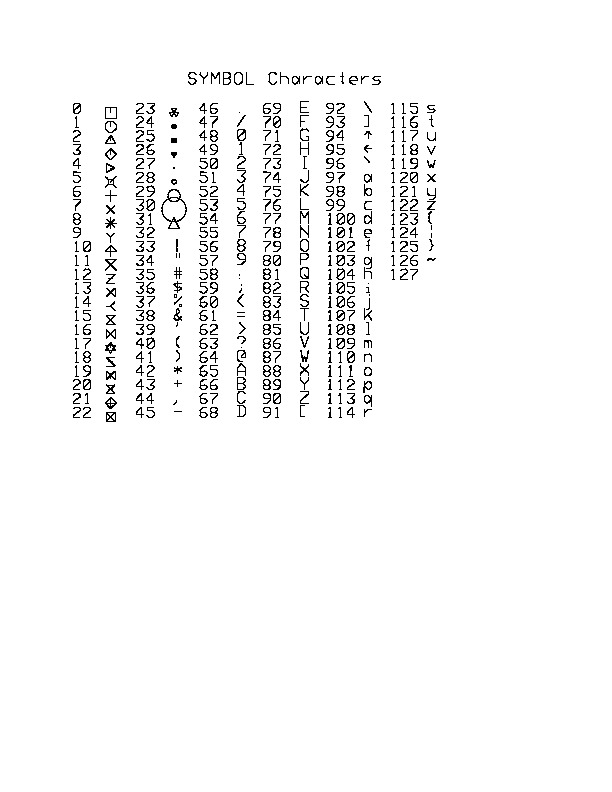
\includegraphics[width=4in]{figures/symbols0.jpg}
\vspace{-2.5in}
\caption{SYMBOL characters for each numerical byte supported. Plot produced by example program
{\tt c/examples/symbols.c}.
\label{fig:symbol}} 
\end{figure}

\section{SUBROUTINE SYMBOL}

The \x{SYMBOL} routine plots an \x{ASCII} string.  Upper and lower
case \x{characters} can be plotted as well as special plotting symbols
and characters.  A list of symbols is shown in the last chapter.  The
plotting symbols 0 to 16 are centered vertically and horizontally,
while other symbols have a reference point on the lower left edge of
the character. Hence, i=-1 should be used for centered plot symbols 0
thru 16.  The number of characters in the input string which should be
plotted can be specified.  If an ASCII null (0) is encountered in the
string beyond the first position, the routine terminates. Examples are
the symbols produced by SYMBOL are shown in Fig.~\ref{fig:symbol}.

The string can be plotted left-justified, centered, or right-justified.
When the string is left-justified, the location of the end of the
plotted string can be optionally returned.  The length of the
plotted string can be computed by calling SYMBOL first with i=-3
and computing the difference between the start and ending points of the
string.

More elaborate characters and different fonts may be obtained using
SYMS. \x{MASTER} routines, \x{AXIS} routines, and \x{NUMBER} all
use \x{SYMBOL} characters.  If the user desires to use \x{SYMS} in
place of SYMBOL throughout a program, the user can add the following
routine to the program.  The subroutine should be titled SYMBOL with
the arguments described below.  This routine simply passes the
arguments (in the same order) to SYMS.
\begin{verbatim}

        SUBROUTINE SYMBOL(x,y,h,s,a,n,i)  ! symbol replacement
        INTEGER S(1)
        A = SYMS(x,y,h,s,a,n,i)           ! call syms
        RETURN
        END
\end{verbatim}
\begin{verbatim}

CALL SYMBOL (x,y,h,s,a,n,i)

x,y   (R): location position (x,y returned if i=-2 or -3)
           If x=999 then x continued from last position in
           prior SYMBOL or NUMBER call. If y=999 then y continued.
h     (R): height of the string to be printed
s     (C): text to be plotted 
a     (R): angle at which the string is to be plotted
n     (I): number of characters in string s to plot
           = -2 : draws pen down to (x,y) before symbol plotted
           = -1 : plots a single symbol
           >  0 : number of characters to plot
i     (I): location flag
            = -3 : same as -2 but string is not plotted and
                   last position is not affected
            = -2 : same as -1 but returns end point in x,y
            = -1 : (x,y) is lower left corner of plotted string
            =  0 : (x,y) is center of plotted array
            =  1 : (x,y) is lower right corner of plotted string
            =  2 : no action
\end{verbatim}


\section{REAL FUNCTION SYMS}

\begin{figure}[htb]
\centering
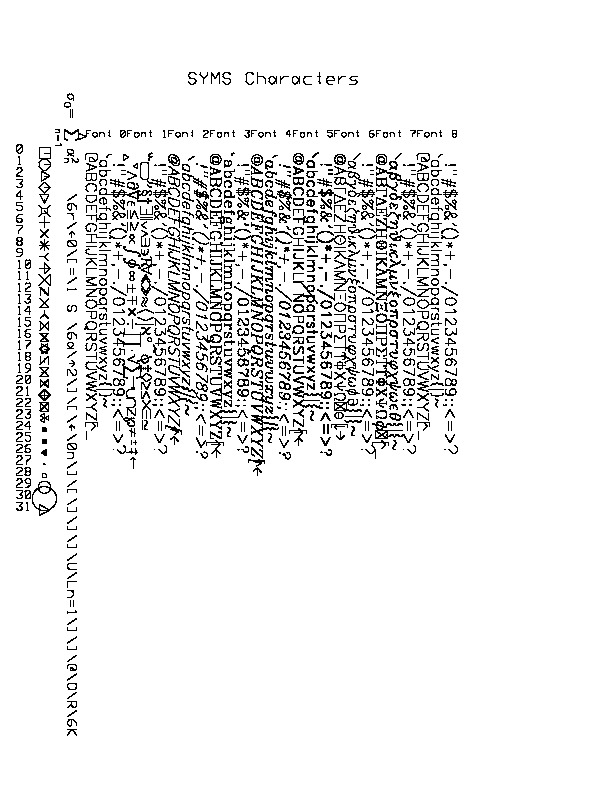
\includegraphics[width=4in,angle=90,origin=c]{figures/symbols1.jpg}
\vspace{-.5in}
\caption{SYMS characters for each numerical byte supported. Plot produced by example program
{\tt c/examples/symbols.c}.
\label{fig:syms}} 
\end{figure}

\index{character plots}\index{SYMBOL}
SYMS plots characters. \x{SYMS} is similar to SYMBOL but provides
additional math and plotting symbols as well as several character
fonts (including \x{Greek} characters), see Fig.~\ref{fig:syms}. SYMS
has primitive positioning capability to permit complicated equations
to be plotted.  All but the 8th font have variable width characters.
The duplex fonts are produce the appearance of solid characters when
the plotting scale is small.  The number of characters in the input
string s plotted and/or interpreted can be specified.  If an ASCII
null (0) is encountered in the string after the first position, the
routine terminates.

The ASCII character ``$\backslash$'' (decimal 93) is used as a control
character to change fonts or subscripting options.  The character
following the ``$\backslash$'' character is interpretted according to
the following table:

\ \\
\centerline{SYMS Options}

\begin{verbatim}
ASCII Character   Decimal       Effect
_______________   _________     ________
     0-9          48-57         Change to font (0-9)
     ; or (space)  59 or 32     Move forward one standard space
      :	           58           Move forward 1/2 standard space
      ,	           44           Move forward 1/4 standard space
      |	          124           Move backward one standard space
      =	           61           Move backward 1/2 standard space
      !	           33           Move backward 1/4 standard space
      @	           64           Reset font, scale, etc. to default values
      _	           95           Begin subscripting
      ]	           93           Back up last character
      ^	           94           Begin superscripting
      [	           91           Reset current level of sub/super script
      L	           76           Move lower 1/2 line
      R	           82           Move higher 1/2 line
      `	           96           Change scale (if next character is
                                  "+" increase scale size by 2
                                  "-" decrease scale size by 2)
      O	           79           Begin over printing
      U            85           Begin under printing

                                Other characters are no-ops
\end{verbatim}
The number of characters in the string should include control characters.

The width of one space is moved when moving forward or backward.  Back
up returns the positioning to the start of the last character.  Up to
6 back up commands can be issued.  Super/sub scripting can be done
recursively.  Only one level is ``popped off'' by the reset current
level of sub/super script.  Scale changes require an additional
character (either a ``+'' or ``-'' to indicate the direction).
Over/under printing permit summation and integral limits to be added.
Fonts are described in the following Table:\\
\ \\
\index{character fonts}
\centerline{Fonts Available in SYMS}
\begin{verbatim}
   Font         Characters      Description
  ______	_____________	____________
    - [all]     ASCII 0-31      Plotting Symbols
    0 [default] ASCII 32-127	Simplex font--variable width
    1           ASCII 32-127    Special math symbols
    2           ASCII 32-127    Simplex Italic
    3           ASCII 32-127    Roman
    4           ASCII 32-127    Roman Italic
    5           ASCII 32-127    Duplex
    6           ASCII 32-127    Simplex Greek
    7           ASCII 32-127    Complex Greek
    8           ASCII 32-127    Crude Simplex--fixed width

\end{verbatim}

For example, the following summation using Greek characters, a
\x{math} symbol, and a super scripted variable can be wrtten:
\begin{verbatim}

  string = \2A\0=\7R\6a\^2\[\]\_\6n\[\]\]\]\=\U\6n=1\@\]\]\O\1K

       infinity    2
    A = SIGMA alpha
       zeta=1     zeta
\end{verbatim}

SYMS is a real function.  The returned value is the final length of the
plotted string.  When i=2 no plotting is done but the length is returned.
When i=-2 the string is plotted and the lower left corner of the next
character position after the end of the string is returned in x,y.
\begin{verbatim}

rlen = SYMS (x,y,h,s,a,n,i)

x,y    (R): string position (x,y returned if i=-2 or i=-3)
            If x=999 then x is continued from last position in
            prior SYMS call.  If y=999 then y continued.
h      (R): height of the string to be printed
s      (C): character variable containing the text to be plotted
a      (R): angle at which the string is to be plotted 
n      (I): number of characters in string s
i      (I): centering flag
            = -3 : same as -2 but string is not plotted and
                   last position is not affected
            = -2 : same as -1 but returns end point in x,y
            = -1 : (x,y) is lower left corner of plotted string
            =  0 : (x,y) is center of plotted array
            =  1 : (x,y) is lower right corner of plotted string
            =  2 : no plotting, plotted length of string returned

rlen   (R): (returned) length of plotted text string
\end{verbatim}


\section{SUBROUTINE VFACTOR}

\x{VFACTOR} is called by \x{FACTOR} to change the input scale conversion factor
for the LONGLIB metafile package.  It may be called separately if desired.
Only the terminal plotting package
is affected.  The routines \x{PFACTOR} and \x{RFACTOR} may be separately 
called to change the input scale conversion factor on the metafile and
Ramtek packages, respectively.  See FACTOR.
\begin{verbatim}

CALL VFACTOR (fac)

fac (R): new conversion factor for coordinate values
         (only the terminal scaling is affected)
         <= 0 : reset scale factor to unity
         >  0 : new scale factor
\end{verbatim}

\section{SUBROUTINE VPEN}

\index{line type}
\index{rmpen}
\index{ppen}
\x{VPEN} is called by \x{NEWPEN} to change the hardware line type and/or width of
the plotting line for subsequent plotting on the terminal screen device.
It may be called separately to change only the terminal line type.
Metafile and Ramtek and terminal output device line types may be changed 
separatly using PPEN and RMPEN, respectively.  While the terminal output
device driver supports line types in hardware, line widths are supported in
software by outputing multiple single-width lines offset by one pixel.
Line type scale factors (the length of the linetype
dot/dash pattern) are not used.  Not all terminals support all
standard line types.  If a particular terminal does not support the
requested line type, normally a solid line is used.
The default line type is a solid line of width 1 dot.
\begin{verbatim}

CALL VPEN (i)

i     (I): selects a line type for all additional plotting
           to the terminal screen output device
           < 0 : resets line type to solid line of unit width.
           = 0 : no change 
           > 0 : line type and width changed according to,
   (1's digit)   : line type (1-9) (0 value does not change line type)
   (10's digit)  : line width (1-7) (0 value does not change width)
   (100's digit) : line type pattern scaling (ignored)
\end{verbatim}

\section{SUBROUTINE WHERE}

\x{WHERE} returns the location from the last call to PLOT. 
The Zoom scale factor value is returned from the LONGLIB graphics device
packages in the priority order: \x{terminal} if open or \x{Ramtek} if open or
else from the metafile.  Does nothing when no device is open.
\begin{verbatim}

CALL WHERE (x,y,z)

x,y   (R): (returned) values of x,y from last call to plot
z     (R): (returned) zoom value.
\end{verbatim}

\section{SUBROUTINE WHEREPR}

\x{WHEREPR}  returns information on the metafile plotting parameters.  If lu <= 0
then metafile has not been initialized.  A routine \x{FIXPR0} (which
has the same parameters) may be used
to set these variables to absolute values without error checking.
\begin{verbatim}

CALL WHEREPR (x,y,ax,ay,z,a,rx,ry,lu,m,iw,ic)

x,y   (R): (returned) current origin
ax,ay (R): (returned) last scaled and shifted origin point
z     (R): (returned) current zoom scale factor
a     (R): (returned) current plotting angle
rx,ry (R): (returned) resolution of metafile
lu    (I): (returned) FORTRAN file output unit number 
                      (if lu <= 0 metafile package not initialized)
m     (I): (returned) current line type
iw    (I): (returned) current line width
ic    (I): (returned) current line color
\end{verbatim}

\section{SUBROUTINE WHERERM}

\x{WHERERM} returns information on the \x{Ramtek} plotting parameters.  If c <= 0
then ramtek has not been initialized.   A routine \x{FIXRM0} (with
same parameters) may be used
to set these variables to absolute values without error checking.
\begin{verbatim}

CALL WHERERM (x,y,z,a,rx,ry,nt,ns,i,ic)

x,y   (R): (returned) current origin
z     (R): (returned) current zoom scale factor
a     (R): (returned) current plotting angle
rx,ry (R): (returned) current pixel resolution
nt    (I): (returned) current line bit pixel pattern
ns    (I): (returned) current line bit scale factor
i     (I): (returned) Ramtek color 
ic    (I): (returned) Ramtek channel
             (if ic <= 0 ramtek is not initialized)
\end{verbatim}

\section{SUBROUTINE WHEREVT}
\index{Selanar}
\index{vt100}
\index{vt125}
\index{vt240}
\index{vt220}

\x{WHEREVT} returns information on the \x{terminal} plotting parameters.  If nv <= 0
then terminal graphics have not been initialized.  A routine
\x{FIXVT0} (with same arguments) may be used to set these variables to 
\x{absolute} values without error checking.
\begin{verbatim}

CALL WHEREVT (x,y,z,a,rx,ry,iv,ns,it,iw,ic)

x,y   (R): (returned) current origin
z     (R): (returned) current zoom scale factor
a     (R): (returned) current plotting angle
rx,ry (R): (returned) current pixel resolution
iv    (I): (returned) terminal code
              (if nv <= 0 terminal is not initialized)
ms    (I): (returned) internal terminal-type code
           = 1 VT100 with Selanar GR100
           = 2 VT125 
           = 3 VT240 
           = 4 VT220 with Selanar GR220
           = 5 Tektronix 4010
           = 6 Tektronix 4109
           = 7 Graphon GO-235
it    (I): (returned) current line type 
iw    (I): (returned) current line width
ic    (I): (returned) current line color
\end{verbatim}

\chapter{Description of 3-d Plotting Routines}
\index{3-d plotting}

The following paragraphs contain detailed descriptions of the
subroutines included in the LONGLIB library for 3-d plotting.  For
added flexibility, two distinct families of 3-d plotting routines have
been provided.  One family is designed for plotting with hidden line
removal; the other family is more flexible but does not perform hidden
line removal.  Both options assume that \x{FRAME} has already been
called, i.e. the plot package is already opened.  The 3-d routines
call \x{PLOT} as output so that the 2-d plot origin, scaling,
rotation, etc. are used in addition to any 3-d operations.

The nominal Z axis of the 3-d plot packages for plotted objects runs out
of the screen.  The X and Y axes are defined as before.

\index{hidden line removal}
Two separate, independent  3-d packages exist.  These are identified by
the initialization routines used for each package.  The hidden line
removal package is \x{INIT3DH} and is a modification of the \x{COSMIC} hidden
line code package (ARC-11446).  The other is INIT3D.  \x{INIT3D} does
not perform any hidden line removal.  These package differ not only in
hidden line removal but also in speed of operation and memory requirements.
The packages are completely independent.  Only routines designed for a
particular package work with that package.  It is possible to
use both simultaneously.

\section{INIT3D Routines}

The INIT3D 3d plotting package permits 3-d plotting but does not include
hidden line removal.
The family of routines used with \x{INIT3D} include:

\begin{enumerate}
\item PLOT3D -- the central plot routine for INIT3D
\item AXIS3D -- plots axes using PLOT3D, NUM3D, and SYM3D
\item NUM3D -- plots numbers using PLOT3D
\item SYM3D -- plots symbols using PLOT3D
\item WHERE3D -- returns the screen coordinates of the last point
drawn by PLOT3D.
\end{enumerate}

The \x{INIT3D} family of 3-d plotting routines are desiged to plot
wireframe line plots with no hidden line removal.  Memory requirements
are modest and plotting is more rapid than for the \x{INIT3DH} routines.
For an example of the use of the INIT3D package see the \x{EXAMP3D}
program included with the LONGLIB graphics library.

\subsection{SUBROUTINE INIT3D}

\x{INIT3D} sets the \x{absolute} origin, rotations, and \x{scale} \x{factor} of
the 3-d package.  These functions are distinct from the functions of
PLOT.  INIT3D may be called at any time to reset these functions without
closing the plot package.  The plot package must be opened with \x{FRAME}
prior to the call to INIT3D.
\begin{verbatim}

CALL INIT3D (x,y,z,xa,ya,za,t,ds,sf,i)

x,y,z    (R): coordinates of view point (looking from)
xa,ya,za (R): coordinates of center point (looking to)
t        (R): rotation angle around line from (x,y,z) to
              (xa,ya,za) in degrees CCW.
ds       (R): perspective scale factor (image size/viewing distance)
sf       (R): relative scale factor
i        (I): plotting flag ( -1 = do not plot, scaling only)
\end{verbatim}

\subsection{SUBROUTINE AXIS3D}
\index{AXIS3}
\index{PLOT3D}
\index{NUM3D}
\index{SYM3D}

\x{AXIS3D} plots an axis and its markings in 3-d.  In order to draw a 
coordinate system, the routine has to be called separately for the x,
y, and z axis.  A possible exponent is determined and placed behind the
axis label in the form of 10**n in the auto scaling mode (see AXIS3).
AXIS3D calls PLOT3D, NUM3D, and SYM3D.  See also AXIS3.
\begin{verbatim}

CALL AXIS3D (x,y,x,a,b,g,s,n,ale,xm,xx,t,c,f)

x,y,z (R): location of start of axis 
a,b   (R): angles from the x-y, x-z planes (in deg) of the ray
           from (x,y,z) along the character string 
g     (R): angle of rotation about the ray defined by a,b (deg)
s     (C): axis title
n     (I): number of characters in the string
           > 0 : axis labelling on positive side (anti-clockwise)
           < 0 : axis labelling on negative side (clockwise)
 (100's digit) = 0 : axis is labeled
               = 1 : line and ticks only--no labeling
ale   (R): length of axis 
           < 0 : tick marks placed on same side of axis as title
           = 0 : no action
           < 0 : tick marks placed opposite side of axis from title
xm    (R): value of first marking on the axis
xx    (R): value of last marking on the axis
t     (R): number of tick marks 
           specification is coded in the form MMM.mmss where
           MMM is the number of major tick marks ( MMM > 0), mm is
           the number of minor tick marks between major tick marks
           (100 > mm => 0), and ss is the number of subminor tick
           marks between minor tick marks (100 > ss => 0).
           (example 1.0102 produces I_._._i_._._I)
c     (R): size of characters 
           < 0 auto exponent scaling (x10 to power) disabled
           > 0 auto exponent scaling (x10 to power) enabled
f     (R): number label format (see NUMBER) 
\end{verbatim}

\subsection{SUBROUTINE NUM3D}
\index{number}
\index{plot3d}

\x{NUM3D} plots a floating point number (see NUMBER) in 3-d using
PLOT3D.  The symbols are plotted in the plane defined by a,b,g.
\begin{verbatim}

CALL NUM3D (x,y,z,a,b,g,f,e)

x,y,z (R): lower-left corner of string
           If x=999, y=999, z=999 then string is continued from
           lower right of previous SYM3D or NUM3D call
a,b   (R): angles from the x-y, x-z planes (in deg) of the ray
           from (x,y,z) along the base of the character string
g     (R): angle of rotation about the ray defined by a,b (deg)
h     (R): height of the number to be plotted
f     (R): number to be plotted
e     (R): format of number representation n.j 
           (see NUMBER for detailed description)
\end{verbatim}

\subsection{SUBROUTINE PLOT3D}
\index{CPLOT3D}

\x{PLOT3D} is the 3-d version of PLOT.  A relative \x{rotation} matrix and
\x{origin} is maintained (separate from viewing matrix and PLOT parameters).
By setting the plotting option flag i in \x{INIT3D} to -1, plotting
is inhibited.  A common block, CPLOT3D, returns a 4 element
vector V with the screen transformed coordinates.  PLOT3D transforms
the 3d input coordinates to 2d coordinates, clips to a 3d clipping
window, and calls \x{PLOT} with the 2d coordinates screen coordinates
of the visible line segments.
\index{screen coordinates}
\begin{verbatim}

CALL PLOT3D (x,y,z,i)

x,y,z (R): coordinates of point (in 3 space)
i     (I): plot function parameter
           =  0: color control
                  x is the line color 
                  if x < 0 the screen is cleared
                  if x >= 0 2d plot angle (PLOT) becomes y
           = -1: change relative scale factor by x
           =  1: change relative rotation matrix
                   rotate x degrees CCW around x axis
                   rotate y degrees CCW around y axis
                   rotate z degrees CCW around z axis
           =  2: draw to (x,y,z) with 'pen down'
           = -2: same as i=2. (x,y,z) becomes new origin
           =  3: move to (x,y,z) with 'pen up'
           = -3: same as i=3. (x,y,z) becomes new origin
           =  9: erase to (x,y,z) (erase is color 0)
           = -9: same as i=9. (x,y,z) becomes new origin

common /CPLOT3D/V(4) : returned screen coordinates (x,y) of last
                       call to PLOT3D  v(1)=x, v(2)=y
\end{verbatim}

\subsection{SUBROUTINE SYM3D}
\index{SYMBOL}

\x{SYM3D} plots an \x{ASCII} string (see SYMBOL) in 3-d using
PLOT3D.  The \x{symbols} are plotted in the plane defined by a,b,g.
\begin{verbatim}

CALL SYM3D (x,y,z,a,b,g,s,n)

x,y,z (R): lower-left corner of string
           If x=999, y=999, z=999 then string is continued from
           lower right of previous SYM3D or NUM3D call
a,b   (R): angles from the x-y, x-z planes (in deg) of the ray
           from (x,y,z) along the base of the character string
g     (R): angle of rotation about the ray defined by a,b (deg)
h     (R): height of the string to be plotted
s     (C): text to be plotted
n     (I): number of characters in string s
\end{verbatim}

\subsection{SUBROUTINE WHERE3D}

\x{WHERE3D} returns the 2d screen coordinates of the last line drawn using
PLOT3D.
\begin{verbatim}

CALL WHERE3D (x,y)

x,y   (R): (returned) screen coordinates of last point
\end{verbatim}

\chapter{Cursor Routines}
\index{INXTCHR}

The routines described in this chapter provide interactive cursor control.
When supported by the terminal, the Tektronix Graphics Inputs (GIN), 
BITCURSOR or GETCURSOR, routines can be used.  If the terminal has
a VT100-compatible text mode, the routines CURMOTION, CURRECT, and CURBAND,
can be used to simulate a GIN device.  These routines use the VT100
keypad and cursor keys.  They rely on a machine-dependent routine
(INXTCHR) to read escape characters from the terminal.  CURMOTION,
CURRECT, and CURBAND return the internal screen "resolution" used
in computing the location of the cursor.  This may not correspond to the
actual hardware resolution of the terminal screen.

The routine CURLOCATE provides
a technique for placing a fixed "cursor mark" on the screen.

A program CURTEST is provided to test and evaluate these cursor routines.

\section{SUBROUTINE BITCURSOR}
\index{cursor}
\index{graphics tablet}
\index{bit pad one}
\index{vt125}

\x{BITCURSOR} moves a cross-hair cursor on a VT100 equipped with a retro-graphics
card (VT125) and a BIT PAD ONE graphics tablet.  The VT125 is used in the
Tek 4010 mode with a graphics point returned when a key is pressed on the
bit pad puck (or stylus).
\begin{verbatim}

CALL BITCURSOR (x,y,k,rx,ry)

x,y (R): (returned) selected cursor position (in plot units)
k   (I): (returned) key code
         = 0  (Z) key pressed on bit pad puck
         = 1  (1) key pressed on bit pad puck
         = 2  (2) key pressed on bit pad puck
         = 3  (3) key pressed on bit pad puck
rx  (R): resolution of screen in x direction (returned)
ry  (R): resolution of screen in y direction (returned)
\end{verbatim}

\index{cursor}
\section{SUBROUTINE CURLOCATE}

\x{CURLOCATE} produces a simulated "x" cursor mark on the screen graphics
device (\x{Ramtek} or \x{terminal} device) When only the metafile is
initialized a call to CURLOCATE is a dummy call.  The terminal takes
precidence over the Ramtek when both are in use.  Erasure of cursor on
requires the correct location where it was first plotted.  CURLOCATE
uses the \x{XOR} capbility of graphics terminal to place and remove
the cursor.  If the terminal has neither erase or XOR capability, the
graphics cursor can not be erased without clearing the entire screen.
If the (x,y) position is off the screen, the cursor is located on
closest edge of the screen to the desired point.
\begin{verbatim}

CALL CURLOCATE (x,y,n,ir)

x,y (R): cursor position
n   (I): cursor number/size (0-4)
         < 0  erase cursor
         > 0  locate cursor
ir  (I): Ramtek cursor control (recognized if Ramtek is output)
         = 0 Ramtek cursor device used
         = 1 plotted Ramtek cursor mark used
\end{verbatim}

\section{SUBROUTINE CURMOTION}

\x{CURMOTION} produces a graphics \x{cursor} on the \x{Ramtek} or \x{terminal}
When no screen devices are initialized a call to CURMOTION is a dummy
call.  Terminal is used in preference to Ramtek.  This routine is
supported only on terminals which can emulate the VT100 numeric
keypad.  The terminal text cursor and VT100 numeric keypad keys are
used to move the graphics cursor to a desired location and a return
function key is pressed to select the cursor location.  Only <space>,
<return>, PF keys and the numeric key pad keys is recognized as
return command keys.  PF1 changes the cursor step movement size in
three sizes. As this happens the cursor changes sizes on the screen.
The cursor position is typed to the terminal when the Ramtek is used.
The cursor is moved in multiples of the pixel resolution.  The formula
below shows the conversion.  All other PF keys and the numeric key pad
keys returns the arguments shown below.  Other keys are not
recognized.  NOTE: The input buffer is 128 characters.  If you exceed
this buffer the program may bomb.  Each cursor key input uses 3
characters.
\begin{verbatim}

     pixel number = (scalefactor * x + origin)/pixelresolution

\end{verbatim}
\begin{verbatim}
CALL CURMOTION (x,y,is,rx,ry)

x,y (R): (returned) selected cursor position
is  (I): (returned) status flag
         < 0  error
         = 0  return key pressed
         = 1  space key pressed
         = 2,3,4 PF2,PF3,PF4 keys on VT100 pressed
         = 10...19 VT100 numeric key pad keys 0...9 pressed
         = 20 numeric key pad period key pressed
         = 21 numeric key pad enter key pressed
         = 22 numeric key pad comma key pressed
         = 23 numeric key pad dash key pressed
rx  (R): resolution of screen in x direction (returned)
ry  (R): resolution of screen in y direction (returned)
\end{verbatim}

\section{SUBROUTINE CURBAND}

CURBAND is similar to the \x{CURMOTION} subroutine except that two
lines are "rubber banded" with the simulated cursor motion.  This
routine is supported only on terminals which can emulate the VT100
numeric keypad.  The line segment rubberbanding can be disabled if
desired.
\begin{verbatim}

CALL CURBAND (x,y,is,rx,ry,x1,y2,x2,y2)

x,y   (R): (returned) selected cursor position
is    (I): (returned) status flag
           < 0  error
           = 0  return key pressed
           = 1  space key pressed
           = 2,3,4 PF2,PF3,PF4 keys on VT100 pressed
           = 10...19 VT100 numeric key pad keys 0...9 pressed
           = 20 numeric key pad period key pressed
           = 21 numeric key pad enter key pressed
           = 22 numeric key pad comma key pressed
           = 23 numeric key pad dash key pressed
rx    (R): resolution of screen in x direction (returned)
ry    (R): resolution of screen in y direction (returned)
x1,y1 (R): starting point of rubber banded line 1
            if x1=999, this line segment is not used
x2,y2 (R): starting point of rubber banded line 2
            if x2=999, this line segment is not used
\end{verbatim}

\section{SUBROUTINE CURRECT}

\x{CURRECT} is similar to the \x{CURBAND} subroutine except that a
\x{rectangle} is moved with cursor motion.  This
routine is supported only on terminals which can emulate the VT100
numeric keypad.
\begin{verbatim}

CALL CURRECT (x,y,is,rx,ry,x1,y2,x2,y2)

x,y   (R): (returned) selected cursor position/start position
is    (I): (returned) status flag
           < 0  error
           = 0  return key pressed
           = 1  space key pressed
           = 2,3,4 PF2,PF3,PF4 keys on VT100 pressed
           = 10...19 VT100 numeric key pad keys 0...9 pressed
           = 20 numeric key pad period key pressed
           = 21 numeric key pad enter key pressed
           = 22 numeric key pad comma key pressed
           = 23 numeric key pad dash key pressed
rx    (R): resolution of screen in x direction (returned)
ry    (R): resolution of screen in y direction (returned)
x1,y1 (R): lower left corner of rectangle
x2,y2 (R): upper right corner of rectangle
\end{verbatim}

\section{SUBROUTINE GETCURSOR}

\x{GETCURSOR} inquires the \x{Tektronix} GIN device for the location
pointed to by the GIN device.  Return code is screen device dependent.
This routine is does support all screen devices.  When a device is not
supported, the routine returns without doing anything.  Screen device
must be in the graphics mode.  GETCURSOR assumes that the \x{GIN}
terminator is a CR (carriage return).  Note: When using an Alpha key
for the return status DO NOT use the <Return> key as this prevents the
correct reading of the returned data.
\begin{verbatim}

CALL GETCURSOR (x,y,k,rx,ry)

x,y (R): (returned) cross-hair location (in LONGLIB coordinates)
k   (I): (returned) GIN status code return (ascii code)
rx  (R): resolution of screen in x direction (returned)
ry  (R): resolution of screen in y direction (returned)
\end{verbatim}

\section{SUBROUTINE RMCURSOR}
\index{cursor}
\index{Ramtek}

\x{RMCURSOR} returns ths position of the Ramtek Package graphics input
device.
\begin{verbatim}

CALL RMCURSOR (x,y,k,b,rx,ry)

x,y (R): (returned) selected cursor position (in plot units)
k   (I): (returned) ASCII key code
         = 0 mouse pressed
b   (I): (returned) mouse button code
         = 0 key pressed
rx  (R): resolution of screen in x direction (returned)
ry  (R): resolution of screen in y direction (returned)
\end{verbatim}


\chapter{MAPPING SUBROUTINES}

\index{map routines}
\index{earth.dat}
\index{lndsea1.dat}

LONGLIB also supports the plotting of maps of the physical earth's surface
by providing mapping routines.
Two data files (EARTH.DAT and LNDSEA1.DAT) are included in the LONGLIB
graphics library package.  EARTH.DAT contains the digitized locations of
the edges of the earth's landmasses.  It forms the basis of a set of 
EARTH OUTLINE mapping routines discussed below.  LNDSEA1.DAT contains a bit map
of land/sea areas.  It forms the basis of the LAND AREA mapping routines discusses
in the second section.

Note: these routines assume that the plot package has already been opened.

\section{EARTH OUTLINE MAPPING ROUTINES}

A small number of routines have been generated for using this data
file.  Current routines allow for plotting the \x{earth} outline map
in 3d or in a linear projection.

A data file (EARTH.DAT) which contains a \x{map} of the land/ocean
interface and a set of routines to access this data has been included
in the LONGLIB graphics library.  The data file (of unknown origin)
contains a list of latitudes and longitudes of the land/ocean edges at
about a 10 km resolution.  It is only a geographic map and does not
contain political boundries.  Although imperfect, it is more than
adequate for large scale map drawing.  It only shows continental
boundaries and not political boundaries.  Due to the high resolution,
the EARTH.DAT file contains a lot of pen motions, requiring a long
plotting time.

Fortran file unit 2 should be reserved for accessing the map data file
by these routines.  The logical name \x{LONGLOC:} must be assigned to
be the location of the EARTH.DAT file.  The routine \x{LNDMAP} is the
general file read routine.  It permits user specified map projection
plotting.

Routines using the land outline file include those for plotting on
3d spheres, flat surfaces, etc.  The general routine is \x{LNDMAP} with
a simple linear 2-d plot in \x{LANDMAP} and a 3-d plot in EARTH3D.

\subsection{SUBROUTINE EARTH3D}

\x{EARTH3D} permits 3d plotting of the earth land map.  This routine
uses the \x{INIT3D} and \x{PLOT3D} 3d graphics package.  It plots
the entire earth map with the option of either a spherical earth or an
ellipsoidal earth.  The radius may be specified.  The transformation
from a latitude/longitude pair (a,b) in radians on the earth's suface
to the 3d plotting vector v is:
\begin{verbatim}

        rad = r * (1 - f*sin(a))
        call sprect1(v,b,a-pi/2,rad)
        call plot3d(v(1),v(2),v(3),2)
where
        pi = 3.141592654
        v is dimensioned v(3)
\end{verbatim}
\begin{verbatim}

CALL EARTH3D(r,f)

r   (R): nominal earth radius (in plotting units)
f   (R): earth flatness
         = 0 for spherical earth
         = 3.3528132e-3 for an ellipsoidal earth
\end{verbatim}

\subsection{SUBROUTINE LANDMAP}
\index{projection}

\x{LANDMAP} plots the earth land edge \x{map} using a linear projection.  The latitude and longitude are assumed to be a linear grid on a flat surface.  It
is a special case of LNDMAP (described below).  By using the PLOT
routine clipping option only parts of the map surface can be plotted
if desired.  Uses Fortran file unit 2.  The transformation of a
latitude/longitude pair (a,b) in degrees to an (x,y) pair for plotting
is:
\begin{verbatim}

        x = (b - s) * along / 360
        y = (a + 90) * alat / 180
\end{verbatim}
\begin{verbatim}

CALL LANDMAP(alat,along,s)

alat  (R): latitude scale factor (plot units/180 deg)
along (R): longitude scale factor (plot units/360 deg)
s     (R): longitude of left-mode edge of map (-180 to +180)
\end{verbatim}

\subsection{SUBROUTINE LNDMAP}
\index{projection}

\x{LNDMAP} plots the earth land edge map using a user-supplied projection
subroutine.  This routine plots the entire map surface.  PLOT
routine clipping option only parts of the map surface can be plotted
if desired.  Uses Fortran file unit 2.

\begin{verbatim}

CALL LNDMAP(proj,s)

proj (EXTERNAL): user-supplied projection subroutine name
s           (R): longitude of left-mode edge of map (-180 to +180)

proj is a subroutine with the call format

CALL MAPPLT(long,lat,ip)

long (R): shifted longitude in deg (0 to 360)
          where "zero" corresponds to the longitude "s"
lat  (R): lattitude in deg (-90 to 90)
ip   (I): "pen" control flag
          = 3: move to (long,lat) with pen up
          = 2: draw to (long,lat) with pen down
\end{verbatim}

An example implementation of proj which uses a linear projection is:
\begin{verbatim}

	SUBROUTINE MAPPLT(ALONG,ALAT,IP)
	DATA XLONG/0.02/ ! LONG. SCALE FACTOR (INCHES/DEG LONG)
	DATA YLAT/0.02/	 ! LAT. SCALE FACTOR (INCHES/DEG LAT)
	X1=ALONG*XLONG
	Y1=(ALAT+90.)*YLAT
	CALL PLOT(X1,Y1,IP)
	RETURN
	END
\end{verbatim}

\subsection{SUBROUTINE POLARMAP}
\index{projection}

\x{POLARMAP} plots the earth land map using a polar projection.  The latitude
is plotted as a linear radius. This routine plots the entire
northern or southern hemisphere.  The transformation from a visible
point (in the appropriate hemisphere) latitude/longitude pair (a,b) in
degrees to a plotted (x,y) pair is:
\begin{verbatim}

        a = b * sgn(r) + a
        x = cos( a * pi / 180) * r / 90 + x0
        y = sin( a * pi / 180) * r / 90 + y0
where
        pi = 3.141592654
\end{verbatim}
\begin{verbatim}

CALL POLARMAP(x0,y0,r,a)

x0,y0  (R): pole location (in plot units)
r      (R): radius of equator (in plot units)
            > northern hemisphere
            < southern hemisphere
a      (R): angle of prime meridian from horizontal (deg CCW)
\end{verbatim}

\subsection{SUBROUTINE SPRECT1}

\x{SPRECT1} converts a \x{spherical} coordinate value (in a latitude/longitude
style spherical system) to \x{rectangular} coordinates.  The
transformation from a latitude/longitude pair (a,b) in degrees to a
rectangular (x,y) pair is:
\begin{verbatim}

        a = b * sgn(r) + a
        x = cos( a * pi / 180) * r / 90 + x0
        y = sin( a * pi / 180) * r / 90 + y0
where
        pi = 3.141592654
\end{verbatim}
\begin{verbatim}

CALL SPRECT1(v,t,p,r)

v  (R): output vector containing rectangular (z,y,z) coordinates
        dimensioned v(3) (returned)
t  (R): theta (longitude) angle (rad)
p  (R): phi (latitude) angle (rad)
r  (R): radius
\end{verbatim}

\section{Land Area Map Routines}
\index{LNDSEA}

The LNDSEA1.DAT file contains a bit \x{map} of the land/sea area of
the earth.  Using the file, a specified point of latitude and
longitude can be determined to be land or sea.  A routine, LNDSEA,
opens the file and provides a flag to indicate if the specified point
is land or sea.

Fortran file unit 1 should be reserved for accessing the map data
file by these routines.  The logical name \x{LONGLOC:} must be assigned
to be the directory containing the LNDSEA1.DAT file.

\subsection{LNDSEA1.DAT Format}

The LNDSEA1.DAT is a direct access file is a world land/sea map
quantized to every 1/12 degree of both latitude and longitude.  An
individual bit is used to indicate whether a particular point is land
or sea.  The data is stored as 648 records each of which contains all
of the data for a 10 degree by 10 degree square.  Each record consists
of 14400 (120*120) bits stored 30 bits per word (4 words per each 1/12
degree strip of data).  The first word of the record indicates whether
the entire 10 by 10 square is all land or water using the following
definition:
\begin{verbatim}

   -1 : square contains both land and sea
    0 : square contains all land
    1 : square contains all water

\end{verbatim}
The next 4 words in each record are the bits for the bottom 1/12 degree
(lowest latitude) row of the 10 degree by 10 degree square with 
longitude bins left to right.  For each bit a 0 indicates land and a
1 indicates water.  The records are ordered:
\begin{verbatim}

 record #  Latitude range  Longitude range
_________ _______________ _________________

   1        -90 to -80         0 to  10
   2        -90 to -80        10 to  20
   .            .                .
  35        -90 to -80       340 to 350
  36        -90 to -80       350 to 360
  37        -80 to -70         0 to  10
  38        -80 to -70        10 to  20
   .            .                .
 648         80 to  90       350 to 360
\end{verbatim}

See the source code for \x{LNDSEA} function for additional information.

\subsection{SUBROUTINE BITMAP}
\index{projection}

\x{BITMAP} plots a land area by testing each point of the area using LNDSEA.
The plotting area is segmented into (nx X ny) regions.  Each point is
tested for the presence of land/sea.  For each resolutoin line of
latitude, a horizontal line is drawn through all points that are land
(or sea as desired).  A linear projection is used.  The latitude and
longitude are assumed to be a linear grid on a flat surface.  This
routine plots the entire map surface.  Use of the PLOT routine
clipping option permits plotting only limited of the map surface
if desired.  The transformation of a latitude/longitude pair (a,b) in
degrees to an (x,y) pair for plotting is:
\begin{verbatim}

        x = (b - s) * along / 360
        y = (a + 90) * alat / 180
\end{verbatim}
\begin{verbatim}

CALL BITMAP(s,alat,along,nx,ny,i)

s          (R): longitude of left-mode edge of map (-180 to +180)
alat,along (R): latitude, longitude axis length (plot units)
nx,ny      (I): x,y resolution specified as the number of lat/longs
                to test for land/sea
i          (I): plot flag
                = 0 plot land area
                = 1 plot sea area
\end{verbatim}

\subsection{INTEGER FUNCTION LNDSEA}
\index{projection}

\x{LNDSEA} tests the point (lat, long) for land/sea using the LNDSEA1.DAT file.
It returns a 0 for land, 1 for sea.  Uses Fortran file unit 1.
\begin{verbatim}

iflag = LNDSEA(alat,along)

alat  (R): latitude (-90. to +90. degrees)
along (R): longitude (0. to +360. degrees)
iflag (I): land/sea flag (returned)
           = -1 : error
           =  0 : land
           =  1 : sea (ocean, lake, sea)
\end{verbatim}



\chapter{MASTER Subroutines}

A set of commonly used general-purpose subroutines for complete
function plots, charts, etc., were included in the LONGLIB graphics
library.  These subroutines are called "MASTER" Subroutines.  Each of
these subroutines is self contained.  When called, it initializes the
plotting package, plots the desired data, and closes the plotting
package.  Often, only one \x{MASTER} subroutine is called in a
program.  However, options are available for multiple calls
to \x{MASTER} subroutines.  Note: when the LONGLIB is initialized by a
MASTER subroutine (which calls FRAME) a metafile using Fortran file
unit 3 is always created. Examples of master routine graphics are
illustrated is Figs.~\ref{fig:plottests1}--\ref{fig:plottests4}.  These
were producted by the example program \xx{PLOTTESTS}.  See additional
examples using MASTER routines are given in the chapter on programming
examples.

To call a MASTER subroutine more than once in a program the option
flag must be set negative for all calls but the last one which should
be positive.  (See also the example \x{PLOTTESTS} program.)  To use
more than one MASTER subroutine in a program:
\begin{enumerate}
\item  On first MASTER subroutine call 
set the option flag negative--this does not close plot package.
\item  on all additional calls to
MASTER subroutines set the option negative and greater than 10000--this
prevents re-opening plot package and does not close it.
\item  On the last call to a MASTER subroutine set option flag positive
but greater than zero--this closes plot package.
\end{enumerate}

\begin{figure}[htb]
\centering
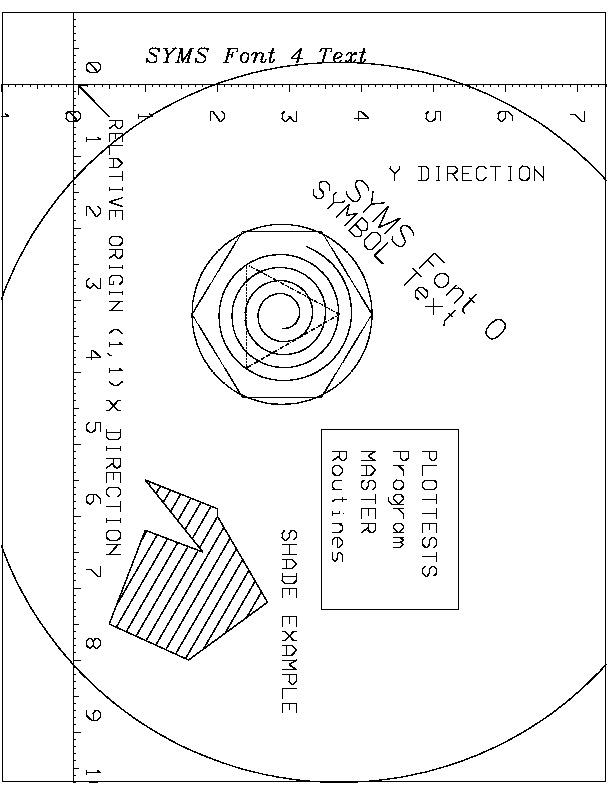
\includegraphics[width=3.5in,angle=90,origin=c]{figures/plottests0.jpg}
\vspace{-.5in}
\caption{PLOTTESTS page 1 output illustrating some plotting capabilities and MASTER routines.
\label{fig:plottests0}} 
\end{figure}

\begin{figure}[htb]
\centering
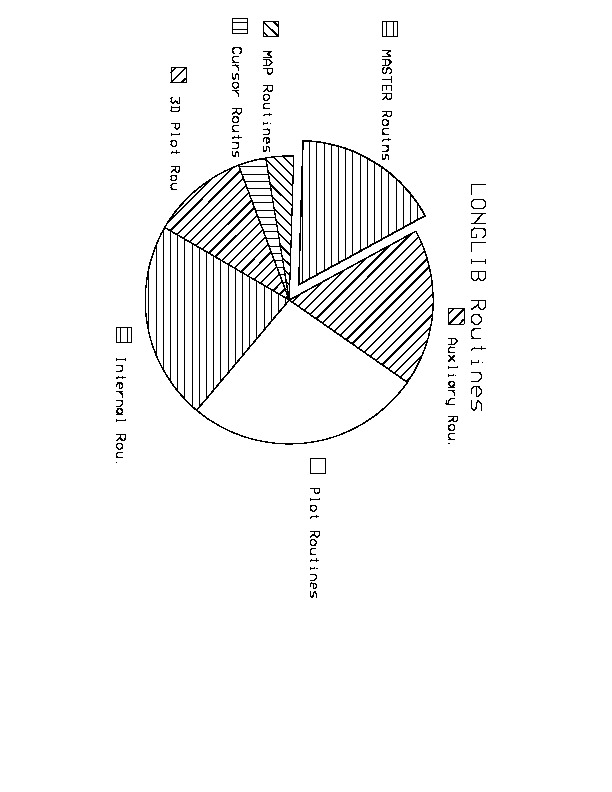
\includegraphics[width=3.5in,angle=90,origin=c]{figures/plottests1.jpg}
\vspace{-.5in}
\caption{PLOTTESTS page 2 output illustrating a pie chart MASTER routine output.
\label{fig:plottests1}} 
\end{figure}

\begin{figure}[htb]
\centering
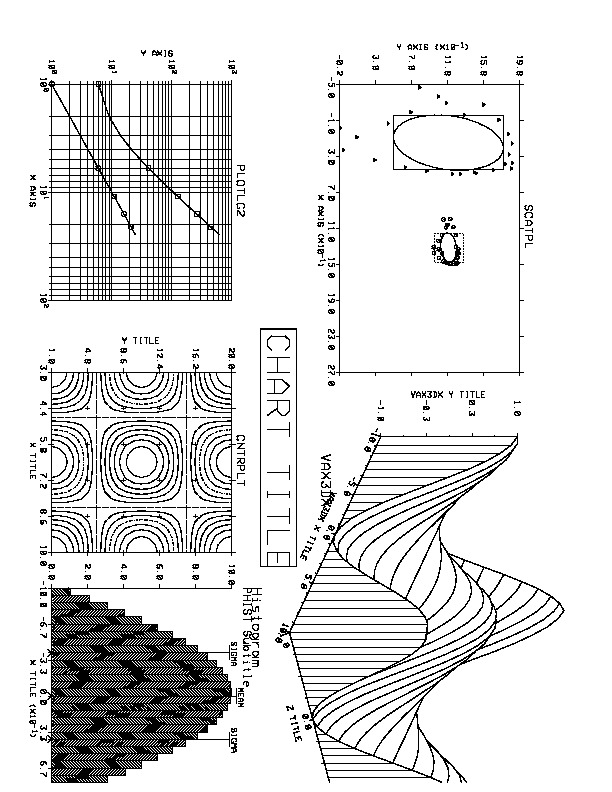
\includegraphics[width=3.5in,angle=90,origin=c]{figures/plottests2.jpg}
\vspace{-.5in}
\caption{PLOTTESTS page 3 output illustrating some MASTER routines.
\label{fig:plottests2}} 
\end{figure}

\begin{figure}[htb]
\centering
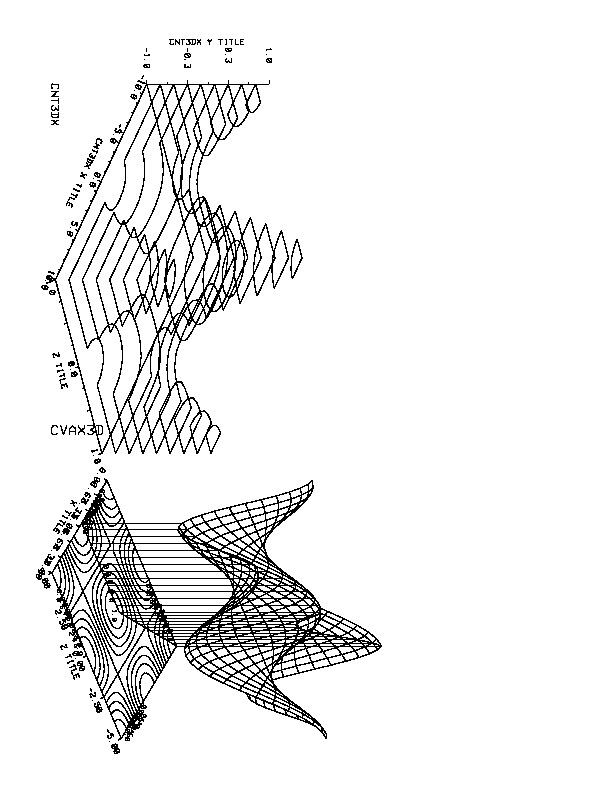
\includegraphics[width=3.5in,angle=90,origin=c]{figures/plottests3.jpg}
\vspace{-.5in}
\caption{PLOTTESTS page 4 output illustrating some MASTER routines.
\label{fig:plottests3}} 
\end{figure}
\clearpage

\begin{figure}[thb]
\centering
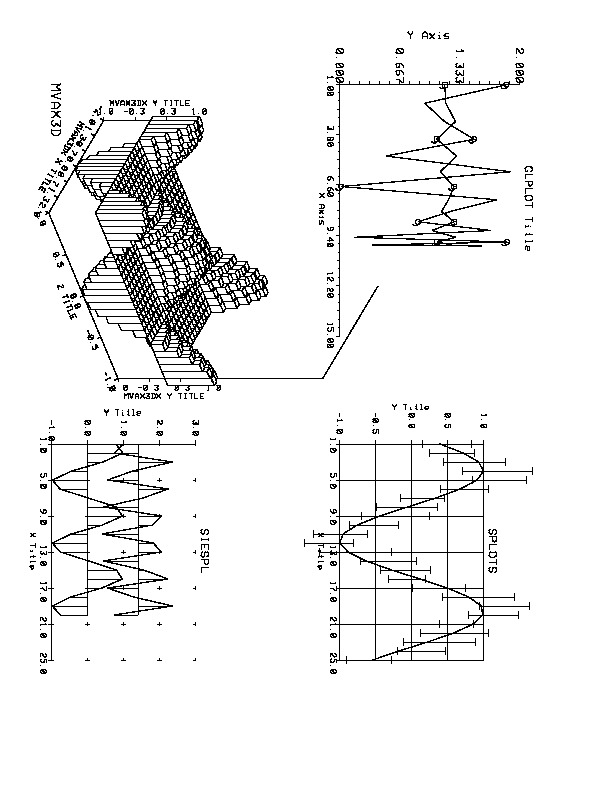
\includegraphics[width=3.5in,angle=90,origin=c]{figures/plottests4.jpg}
\vspace{-.5in}
\caption{PLOTTESTS page 5 output illustrating some MASTER routines.
\label{fig:plottests4}} 
\end{figure}

In summary, when LONGLIB is already open set the magnitude of the
option flag to greater than 10000.  To prevent closing the plot
package set option flag negative.  When the plot package is closed in
a MASTER subroutine CTERM(-2) is used to ask if a termina lscreen
clear (terminal plotting only) should be done.  MASTER subroutines
always return the terminal to the text mode after call.  When color
options are enabled, the color marked "(return)" is the color in
current use after call.
\index{common block}

Most MASTER subroutines have \x{common} blocks with the same name
prefixed with the letter "C" which contain the scaling information
used to plot the data line. This can be useful for plotting additional
annotations, etc.

The following pages document the currently defined MASTER Subroutines. 
Additional subroutines may be added as suggested by the users.

\section{MASTER Routine Index}

The sections that follow detail each MASTER routine.  A brief index
of the capabilities of each Master routine is given below.  To select
a MASTER routine, determine the category of plotting needed and
look at the available MASTER routine capabilities.  For general purpose
line plotting where flexibility in specifying the axes,
the routine GLPLOT is recommended.

\subsection{Pie Chart}
\begin{enumerate}
\item  PICHRT
\end{enumerate}

\subsection{Bar Chart}
\begin{enumerate}
\item  BARCHR 
\end{enumerate}

\subsection{Single linear/linear line}
\begin{enumerate}
\item  PLOTSC (simple)
\item  GLPLOT (flexible axis specification)
\item  PLOTLGXL (allows log lines, software line types)
\item  LSPLOT (options via array)
\end{enumerate}

\subsection{Two linear/linear lines on the same plot}
\begin{enumerate}
\item  PLOTSC2  (simple)
\item  GLPLOT   (flexible axis specification)
\item  PLOTLG2  (allows log lines)
\item  PLOTLGX  (allows log lines, flexible axis specification)
\item  PLOTLGXL (allows log lines, software line types)
\item  BARCHR   (can fill area between lines)
\item  LSPLOT (options via array)
\end{enumerate}

\subsection{Multiple linear/linear lines on the same plot}
\begin{enumerate}
\item  GLPLOT   (more complex but flexible axis specification)
\item  PLOTLGX  (allows log lines, flexible axis specification)
\item  PLOTLGXL (software line types)
\item  SEISPL   (special options)
\item  SPLOTS   (can show error bars)
\item  SPLOTSX  (can show error bars with flexible axis)
\item  BARCHR   (can fill area between lines)
\item  LSPLOT (options via array)
\end{enumerate}

\subsection{Multiple log/linear or log/log lines on the same plot}
\begin{enumerate}
%\item  PLOTLG  (relatively simple)
%\item  PLOTLGX (more complex, flexible axis specification)
\item  GLPLOT (options in call)
\item  LSPLOT (options via array)
\end{enumerate}

\subsection{Scatter plot}
\begin{enumerate}
\item  SCATPL
\item  SPLOTS  (can show error bars)
\item  SPLOTSX (can show error bars with flexible axis)
\item  SEISPL  (special options)
\item  LSPLOT (options via array)
\end{enumerate}

\subsection{1-d Histogram}
\begin{enumerate}
\item  PHIST  (can show mean/standard deviation)
\item  BARCHR (bar chart)
\end{enumerate}

\subsection{Lines/points with error bars}
\begin{enumerate}
\item  SPLOTS (simple)
\item  SPLOTSX (flexible axis specification)
\item  LSPLOT (options via array)
\end{enumerate}

\subsection{Special plot formats}
\begin{enumerate}
\item  SEISPL (forms used in seismic data plots)
\item  BARCHR (bar chart)
\item  PICHRT (pie chart)
\item  LSPLOT (options via array)
\end{enumerate}

\subsection{Contour Plot with equally spaced data}
\begin{enumerate}
\item  CNTRLN (simple, robust)
\item  LCNTR  (simple, less-robust, contour line types and labels)
\end{enumerate}

\subsection{Contour Plot with unequally spaced data}
\begin{enumerate}
\item CNTLN  (triangulates points then contours)
\end{enumerate}

\subsection{3-d Surface slices}
\begin{enumerate}
\item  VAX3D  (simple)
\item  VAX3DX (more complex, with flexible axis specification)
\end{enumerate}

\subsection{3-d Surface mesh (no hidden line removal):}
\begin{enumerate}
\item  MESH3D  (simple)
\item  MESH3DX (more complex, with flexible axis specification)
\end{enumerate}

\subsection{3-d Surface mesh (hidden line removal)}
\begin{enumerate}
\item  MVAX3D  (simple)
\item  MVAX3DX (more complex, with flexible axis specification)
\end{enumerate}

\subsection{3-d Surface mesh with contour plot (hidden line removal)}
\begin{enumerate}
\item  CVAX3D  (simple)
\item  CVAX3DX (more complex, with flexible axis specification)
\end{enumerate}

\subsection{3-d Surface triangular mesh (hidden line removal)}
\begin{enumerate}
\item  T3DH (uses INIT3DH)
\end{enumerate}

\subsection{Unequally sampled 3-d Surface (hidden line removal):}
\begin{enumerate}
\item  TRIG3DH (uses INIT3DH)
\end{enumerate}

\subsection{3-d Histogram with hidden line removal}
\begin{enumerate}
\item  HIST3D (uses INIT3DH)
\item  MVAX3D (simple)
\item  MVAX3DX (more complex, with flexible axis specification)
\item  CVAX3D (simple, can include contour plot)
\item  CVAX3DX (with flexible axis specification, with contour plot)
\end{enumerate}

\subsection{3-d Contour Plot with equally spaced data (no hidden line removal)}
\begin{enumerate}
\item  CNT3D  (simple, robust)
\item  CNT3DX (more complex, with flexible axis specification)
\end{enumerate}

\subsection{4/5-d Surface plots:}
These are not available in all installations.
\begin{enumerate}
\item  VAX5D  (slices)
\item  MVAX5D  (mesh/histogram with hidden line removal)
\end{enumerate}


\newpage
\section{SUBROUTINE BARCHR}

\x{BARCHR} plots a bar chart with optionally shaded bar segments and
descriptive legends.  In addition, multiple lines with shading between
lines can be plotted.  Legend can be automatically placed
or the user can specify the location of the legend.  In the bar chart
mode, bars can run vertically or horizontally.
b(i,j) specifies the ith bar and jth segment of bar (or horizontal line
depending on iflag option).  Top of jth segment or height of jth line
is computed from:
\begin{verbatim}

                       j
   yplotted = ylen * (Sum b(i,k) - bm)/(bx-bm)
                      k=1
\end{verbatim}
\begin{verbatim}

CALL BARCHR(b,nb,ns,sh,iflag,xl,yl,bm,bx,f,nd,sp,sl,nsl,bl,nbl,cs
              t,nt,bt,nbt,lt,nlt,tcs,a,d,ip,ic)

b     (R): bar data array dimensioned b(nb,ns)
nb    (I): number of bars/number of points in each line
ns    (I): number of segments in each bar/number of lines
sh    (I): shade option for segment/area between lines
           dimensioned sh(ns)
              sh            shade pattern
             ____       _________________________
              0               no shading
              1          -45 deg solid lines
              2          horizontal solid lines
              3          +45 deg solid lines
              4          vertical deg solid lines
              5          -45 deg dotted lines
              6          horizontal dotted lines
              7          +45 deg dotted lines
              8          vertical deg dotted lines
              9          +/- 45 deg dotted lines
             10          vertical/horizontal dotted lines
             11          +/- 45 deg solid lines
             12          vertical/horizontal solid lines
iflag (I): option flag
           < 0 : do not close LONGLIB after plotting
           = 0 : close LONGLIB--no plot produced
           > 0 : close LONGLIB after plotting
(magnitude) > 10000 : do not initialize LONGLIB before plotting
   (1's digit)  = 1 : color array not used
                = 2 : color array used
   (10's)       = 0 : bar chart with vertical bars
                = 1 : bar chart with horzontal bars
                = 2 : multiple line chart
   (100's)      = 0 : Ask which screen device to use
               <> 0 : Screen Device Number (see FRAME)
xlen  (R): length of horizontal axis
           < 0 : chart is enclosed in a box
           > 0 : only bottom and left axes plotted
ylen  (R): length of vertical axis
bm,bx (R): minimum and maximum values to be shown on chart
           note: if bx=bm, values computed from b array will be used
f     (R): format for numeric labels on axis (see NUMBER)
nd    (I): number of divsions of bar length axis
           < 0 : division lines shown on chart
           = 0 : no division lines or numeric labels
           > 0 : division lines shown
sp    (R): width of bar (ignored for line plot)
           = 0 : auto scaling with evenly spaced bars
           > 0 : bars grouped in groups of int(sp).  Each
                 bar has width frac(sp).
sl    (C): segment legend labels (CHARACTER data type)
           dimensioned sl(ns)
nsl   (I): number of characters to use in plotting sl's
           = 0 : no label plotted
bl    (C): bar labels (CHARACTER data type) dimensioned bl(nb)
nbl   (I): number of characters to use in plotting bl's
           = 0 : no label plotted
cs    (R): legend/bar label character height
t     (C): title string placed on top of chart
nt    (I): number of characters in t
           = 0 : no label plotted
bt    (C): title string placed at base of bars
nbt   (I): number of characters in bt
           = 0 : bt not plotted
lt    (C): title string placed on bar length axis
nlt   (I): number of characters in lt
           = 0 : lt not plotted
tcs   (R): height of title strings
a     (R): legend location/shading box size dimensioned a(3)
            a(1) : legend box size
                   < 0 : legend placed to right of chart, a(2)
                         and a(3) are not used
                   = 0 : no legend
                   > 0 : a(2) and a(3) used to locate legend
            a(2) : x position of lower left corner of legend
            a(3) : y position of lower left corner of legend
d     (R): distance between shading lines
           < 0 : line width array used
           > 0 : line width array not used
ip    (I): line width array (used only if d<0)
            p(1) : axis line width
            p(2) : division line width
            p(3) : bar outline/data line width
            p(4) : labeling line width
            p(5) : title line width (bt,lt)
            p(6) : title line width (t)
ic    (I): color array (used only if mod(|iflag|,10)=2)
            c(1) : t title color (return)
            c(2) : bt title color
            c(3) : lt title color
            c(4) : axis numberic label colors
            c(5) : sl label color
            c(6) : bl label color
            c(7) : segment 1 color
            c(8) : segment 2 color
            ...         ...
\end{verbatim}

\newpage
\section{SUBROUTINE CNT3D}

CNT3D plots a simple 3-d contour of equally spaced points with no hidden
line removal. (see CNT3DX)
\x{CNT3D} calls CNT3DX using default axis parameters to simplify calling
procedure.
\begin{verbatim}

CALL CNT3D(d,ndx,ndz,nx,nz,a,b,xh,yh,zh,nl,as,ae,ie,iflag,iax,
              <xt,nxt,xs,xe,yt,nyt,zt,nzt,zs,ze,<dm,dx<,ic>,l>>>)

See CNT3DX for parameter description.
 (iax is limited to a single digit value)
\end{verbatim}
\section{SUBROUTINE CNT3DX}

\index{3-d contour plot}
\x{CNT3DX} is a simple 3-d contour plotting routine.  A 3-d surface is
contoured by plotting slices through the surface parallel to the x-z plane
of the surface which have the same y value.  The input consists of a 2
dimensional grid of y values.  For each contour level the input array
is scanned cell-by-cell.  A segment of the contour is determined by linearily
interpolating the edges of the square formed by 4 adjacent points (a cell).
For example, if the current contour value is 1, and y(1,1)=0, y(1,2)=2,
y(2,2)=3, and y(1,2)=4, a contour line is assumed to exist for this
cell as shown:
\begin{verbatim}

         y(1,2)      y(2,2)
        *          *
 
        +
         \
        * +        *
         y(1,1)      y(1,2)

\end{verbatim}
This line segment is plotted using the same approach as \x{VAX3DX}.
No hidden line removal is provided.  The calling sequence is nearly
identical for both CNT3DX and VAX3DX. The height of plotted contours
relative to the y axis is calibrated to z axis so that scale can be
taken from the plot.  No perspective is used.  Options exist to vary
the plotting angle and to plot axes.  Contour values can be
distinguished by color and/or line type.

Origin of the plot is in the lower-left corner.  The x axis runs
plotted left to right along the plot bottom.  The y axis is plotted
as a vertical displacement offset by the z axis value.  The z axis appears
to point into the screen.  This gives the illusion of depth in the plot.
See AXIS2 for detailed discription of axis parameters.

The pathological case of two contour lines within a cell may case the
routine to incorrectly trace the contour through that cell.
\begin{verbatim}

CALL CNT3DX(d,ndx,ndz,nx,nz,a,b,xh,yh,zh,nl,as,ae,ie,iflag,iax,
               <xt,nxt,xs,xe,nmx,nnx,mlx,tsx,ndx,smx,
                yt,nyt,nmy,nny,mly,tsy,ndy,smy,
                zt,nzt,zs,ze,nmz,nnz,mlz,tsz,ndz,smz,
               <dm,dx<,ic>,l>>>)

d        (R): array of y values dimensioned d(ndx,ndz)
ndx,ndz  (I): x and z dimensions of d array
nx,nz    (I): x and z sizes of surface to plot d array
a        (R): angle of x axis from horizontal 0-85 degrees
b        (R): angle of z axis from horizontal 0-90 degrees
              note: origin d(1,1) is in lower-left corner
              x axis runs left to right on screen
              y axis runs up to down on screen
              z axis appears to run into the screen but is angled
                   to the right
xh,yh,zh (R): length of each axis
nl    (I): number of uniformly spaced contour levels,
           < 0 : max and min of v are used for as, ae
                 (j)th contour is (j-1)*(ae-as)/(nl-1)+as
           = 0 : int(ae) specifies the number of contour values
                 where as is an array of the contour values
           > 0 : number of uniformly space contour levels,
                 (j)th contour is (j-1)*(ae-as)/(nl-1)+as
as    (R): first contour level (nl > 0)
           array of contour levels (nl=0) dimensioned as(int(ae))
ae    (R): last contour level (nl > 0)
           number of contour levels in as (nl=0) ae>0
ie    (I): contour edge option flag
           < 0 contour edge added when surface below contour
           = 0 no contour edges added
           > 0 contour edge added when surface above contour
iflag (I): option flag
           < 0 : do not close LONGLIB after plotting
           = 0 : close LONGLIB--no plot produced
           > 0 : close LONGLIB after plotting
(magnitude)  >10000: do not initialize LONGLIB before plotting
   (1's digit) = 1 : ignor color and line type arrays
                 2 : use color array but not line type array
                 3 : ignore color array, use line type array
                 4 : use color and line type arrays
   (10's digit)= 0 : Ask which screen device to use
              <> 0 : Screen Device Number (see FRAME)
iax   (I): axis format control
           < 0 : plot axis, using input scale factors dm and dx
           = 0 : do not plot axis, optional axis parameters not used
                 input scaling is computed from input array
           > 0 : plot axis, using scaling computed from input array,
                 need optional axis parameters
 (1's digit)  = 1 : Plot actual max/min or input values for Y axis
              = 2 : Plot smoothed values for Y axis
 (10's digit) = 0 : Use default axis type
              = 1 : Use input AXIS2-type axis parameters
(NOTE: the following optional parameters are used only if iax<0 or 
       mod(iflag,10)=1)
xt    (C): title of x axis (width)
nxt   (I): number of characters in xt
           = 0 : no axis plotted
           > 0 : normal
xs,xe (R): starting and ending values displayed on x axis
(see AXIS2 for detailed description of axis parameters)
nmx   (I): number of minor ticks between major ticks on x axis
nnx   (I): highlight length of nnx-th minor tick on x axis
mlx   (I): number of major tick marks on x axis
tsx   (R): size of title and numbers on x axis
           < 0 auto exponent scaling (x10 to power) disabled
           > 0 auto exponent scaling (x10 to power) enabled
ndx   (I): number of digits to right of decimal point on x axis
smx   (R): major tick length on x axis
yt    (C): title of y axis (depth)
nyt   (I): number of characters in yt
           = 0 : no y axis plotted
           > 0 : normal
nmy   (I): number of minor ticks between major ticks on y axis
nny   (I): highlight length of nny-th minor tick on y axis
mly   (I): number of major tick marks on y axis
tsy   (R): size of title and numbers on y axis
           < 0 auto exponent scaling (x10 to power) disabled
           > 0 auto exponent scaling (x10 to power) enabled
ndy   (I): number of digits to right of decimal point on y axis
smy   (R): major tick length on y axis
zt    (C): title of z axis (height)
nzt   (I): number of characters in zt
           = 0 : no z axis plotted
           > 0 : normal
ze,ze (R): starting and ending valued displayed on z axis
nmz   (I): number of minor ticks between major ticks on z axis
nnz   (I): highlight length of nnz-th minor tick on z axis
mlz   (I): number of major tick marks on z axis
tsz   (R): size of title and numbers on z axis
           < 0 auto exponent scaling (x10 to power) disabled
           > 0 auto exponent scaling (x10 to power) enabled
ndz   (I): number of digits to right of decimal point on z axis
smz   (R): major tick length on z axis
(NOTE: the following are accessed only if iax<0 or mod(iflag,10)<>0)
dm,dx (R): minimum and maximum values of d array
(NOTE: the following is accessed only if mod(iflag,10) <> 0)
ic    (I): color array
           ic(1) : color for axis lines
           ic(2) : color for axis numbers
           ic(3) : color for axis titles
           ic(4) : color for axis exponents
           ic(5) : color for contour line 1
           ic(6) : color for contour line 2, etc.
            ...      ...
l     (I): contour linetype list
\end{verbatim}

\newpage
\section{SUBROUTINE CNTLN}

\index{contour plot}
\x{CNTLN} plots a contour plot of a randomly scattered set of points in
three dimensions.  The input consists of a list of triplets of a surface
value.  The triplets are triangulated using \x{TRIANGC} and contours
determined by linearily interpolating the edges of the triangles.
The contour values may be uniformly spaced between the starting
and end values or from a list.  Other than color, the
sequence of plotting (min to max), and line typing of various contour
lines, no contour line identification scheme is provided.  Caution
should be exercised when interpreting plot since the distribution of
input points may affect the placement of the contour lines.
\begin{verbatim}

CALL CNTLN(x,y,z,n,xl,yl,iflag,nc,c,ia,xt,nxt,tx,sx,fx,
                yt,nyt,ty,sy,fy,t,nt,xm,xx,ym,yx<<,ic>,l>)

x,y,z (R): array of point triplets (x,y,z)
n     (I): number of points
xl    (R): x axis length in inches
yl    (R): y axis length in inches
iflag (I): option flag
           < 0 : do not close LONGLIB after plotting
           = 0 : close LONGLIB--no plot produced
           > 0 : close LONGLIB after plotting
(magnitude)  >10000: do not initialize LONGLIB before plotting
   (1's digit)   = 1 : do not use color or line type arrays
                 = 2 : use color but not line type array
                 = 3 : do not use color but use line type array
                 = 4 : use both color and line type arrays
   (10's digit)  = 0 : just x,y labeled axes
                 = 1 : axes and axis line/ticks on top and sides
   (100's digit) = 0 : Ask which screen device to use
                <> 0 : Screen Device Number (see FRAME)
nc    (I): number of contour levels 
           < 0 : c(1) is the minimum contour level and c(2) is
                 the contour step size, abs(nc) levels plotted
           > 0 : c contains contours levels, c dimensioned c(nc)
c     (R): list of contour levels
ia    (I): axis option flag
          < 0 : do not plot axes
          > 0 : plot axes
   (1's digit)   = 1 : plot y axis using max/min of y array
                 = 2 : plot y axis using max/min of y array
                       smoothed by SCALE
                 = 3 : plot y axis using input max/min
                 = 4 : plot y axis using input max/min
                       smoothed by SCALE
   (10's digit)  = 1 : plot x axis using max/min of x array
                 = 2 : plot x axis using max/min of x array
                       smoothed by SCALE
                 = 3 : plot x axis using input max/min
                 = 4 : plot x axis using input max/min
                       smoothed by SCALE
   (100's digit) = 0 : normal contouring
                 = 1 : show triangulation used without contours
xt     (C): x axis title string
nxt    (I): number of characters in title
           < 0 : axis ticks on top of x axis
           = 0 : no axis
           > 0 : axis ticks on bottom of x axis (normal)
tx     (R): number and pattern of axis ticks (see AXIS3)
sx     (R): size of axis labeling (see AXIS3)
           < 0 auto exponent scaling (x10 to power) disabled
           > 0 auto exponent scaling (x10 to power) enabled
fx     (R): format of axis number labeling (see AXIS3)
yt     (C): y axis title string
nyt    (I): number of characters in title
           < 0 : axis ticks on top of x axis
           = 0 : no axis
           > 0 : axis ticks on bottom of x axis (normal)
ty     (R): number and pattern of axis ticks (see AXIS3)
sy     (R): size of axis labeling (see AXIS3)
           < 0 auto exponent scaling (x10 to power) disabled
           > 0 auto exponent scaling (x10 to power) enabled
fy     (R): format of axis number labeling (see AXIS3)
t      (C): plot title string
nt     (I): number of characters in t (limited to 99 characters)
            < 0 : use color array
            = 0 : no title
            > 0 : do not use color array
            if |nt|/100 > 0 : use line type list
xm     (R): minimum value of x axis
xx     (R): maximum value of x axis
ym     (R): minimum value of y axis
yx     (R): maximum value of y axis
ic     (I): color list (optionally used)
            ic(1) : color for axis lines
            ic(2) : color for axis numbers
            ic(3) : color for axis titles
            ic(4) : color for axis exponents
            ic(5) : color contour (1)
            ic(6) : color contour (2), etc.
             ...      ...
l      (I): line type list for contours (optionally used)

common /ccntrplt/xmr,dxr,ymr,dyr

xmr   (R): returned value of xmin
dxr   (R): returned value of scale factor (xmax-xmin)/xlen
ymr   (R): returned value of ymin
dyr   (R): returned value of scale factor (ymax-ymin)/ylen
\end{verbatim}

\newpage
\section{SUBROUTINE CNTRPLT}

\index{contour plot}
\x{CNTRPLT} plots a contour plot of a uniformly sampled 2-d input
array.  The input consists of a 2 dimensional grid of y values.  For each
contour level the array is scanned cell by cell.
A contour segment is determined by linearily interpolating the edges of the
square formed by 4 adjacent points (a cell).  For example, if the current
contour value is 1, and y(1,1)=0, y(1,2)=2, y(2,2)=3, and y(1,2)=4,
a contour line is assumed to exist for this cell as shown:
\begin{verbatim}

         y(1,2)        y(2,2)
        *          *

        +
         \
        * +        *
         y(1,1)        y(1,2)

\end{verbatim}
The contour values are uniformly spaced between the input starting
and end values or automatically selected values.  Other than color, the
sequence of plotting (min to max), and line typing of various contour
lines, no contour line identification scheme is
provided. Log axes are available but data points are plotted using
linear positioning.  (Note: common block scale factors are log values
if the log axes are selected.)

The pathological case of two contour lines within a cell may case the
routine to incorrectly trace the contour through that cell.
\begin{verbatim}

CALL CNTRPLT(v,ndx,ndy,nx,ny,nl,as,ae,iflag,xl,yl,xt,nxt,yt,nyt,
                t,nt,xm,xx,ym,yx<<,ic>,l>)

v       (R): 2-d array dimensioned v(ndx,ndy)
ndx,ndy (I): dimensions of v data array
nx,ny   (I): number of points in each array dimension
nl      (I): number of uniformly spaced contour levels,
             < 0 : max and min of v are used for as, ae
                   (j)th contour is (j-1)*(ae-as)/(nl-1)+as
             = 0 : int(ae) specifies the number of contour values
                   where as is an array of the contour values
             > 0 : number of uniformly space contour levels,
                   (j)th contour is (j-1)*(ae-as)/(nl-1)+as
as      (R): first contour level (nl > 0)
             array of contour levels (nl=0) dimensioned as(int(ae))
ae      (R): last contour level (nl > 0)
             number of contour levels in as (nl=0) ae>0
iflag   (I): option flag
             < 0 : do not close LONGLIB after plotting
             = 0 : close LONGLIB--no plot produced
             > 0 : close LONGLIB after plotting
(magnitude)  >10000: do not initialize LONGLIB before plotting
   (1's digit)   = 1 : plot x linear, y logarithmic (base 10)
                 = 2 : plot x logarithmic, y linear
                 = 3 : plot x logarithmic, y logarithmic
                 = 4 : plot x linear, y linear
   (10's digit)  = 0 : no axes or title plotted
                 = 1 : plot box with axis tick marks on top and sides
                 = 2 : plot solid cartesian grid
                 = 3 : plot ticked cartesian grid without box
                 = 4 : plot ticked cartesian grid with box
                 = 5 : plot ticked cartesian grid, box w/axis ticks
                 = 6 : plot without box or cartesian grid
                 = 7 : plot solid logarithmic grid
                 = 8 : plot dotted logarithmic grid
                 = 9 : plot ticked logarithmic grid
   (100's digit) = 0 : Ask which screen device to use
                <> 0 : Screen Device Number (see FRAME)
xl    (R): x axis length in inches (integer-valued)
           > 0 : use input scaling in xm,xx for axis
           < 0 : use smoothed input scaling in xm,xx for axis
yl    (R): y axis length in inches (integer valued)
           > 0 : use input scaling in ym,yx for axis
           < 0 : use smoothed input scaling in ym,yx for axis
xt    (C): x axis title string
nxt   (I): number of characters in xt
           < 0 : axis ticks on top of x axis
           = 0 : no axis
           > 0 : axis ticks on bottom of x axis (normal)
yt    (C): y axis title string
nyt   (I): number of characters in yt
           < 0 : axis ticks on right of y axis
           = 0 : no axis
           > 0 : axis ticks on left of y axis (normal)
t     (C): plot title string
nt    (I): number of characters in t (limited to 99 characters)
           < 0 : use color array
           = 0 : no title
           > 0 : do not use color array
           if |nt|/100 > 0 : use line type list
xm    (R): minimum value of x axis (will be smoothed for xl < 0) 
xx    (R): maximum value of x axis (will be smoothed for xl < 0) 
ym    (R): minimum value of y axis (will be smoothed for yl < 0) 
yx    (R): maximum value of y axis (will be smoothed for yl < 0) 
(NOTE: color array accessed if nt < 0 or |nt|/100 >0)
ic    (I): color array 
           ic(1) : color for grid
           ic(2) : color for axis lines
           ic(3) : color for axis numbers
           ic(4) : color for axis titles
           ic(5) : color for axis exponent
           ic(6) : color for title (return)
           ic(7) : color for contour line 1
           ic(8) : color for contour line 2
           ic(9) :    etc. ...
l     (I): line type list for contours (accessed only if |nt|/100>0)

common /ccntrplt/xmr,dxr,ymr,dyr

xmr   (R): returned value of xmin
dxr   (R): returned value of scale factor (xmax-xmin)/xlen
ymr   (R): returned value of ymin
dyr   (R): returned value of scale factor (ymax-ymin)/ylen
\end{verbatim}

\newpage
\section{SUBROUTINE CVAX3D}

CVAX3D plots a 3d surface with hidden line removal using either
a mesh or a histogram.  Optionally, a contour plot can be included
beneath the surface.  The vertical space may be specified.
See CVAX3DX.
\x{CVAX3D} calls CVAX3DX using default axis parameters to simplify the calling
procedure.
\begin{verbatim}

CALL CVAX3D(d,ndx,ndz,nx,nz,a,b,xh,yh,zh,iflag,
               iax,ds,nc,cv,icl,nm,il,ip,
               <xt,nxt,xs,xe,yt,nyt,zt,nzt,zs,ze,<dm,dx<,ic>>>)
\end{verbatim}

\section{SUBROUTINE CVAX3DX}

\index{2-d surface plot}
\x{CVAX3DX} plots a 3-d surface with hidden lines removed using \x{PLT3D} to
produce a mesh surface or \x{HLT3D} to produce a 2-d histogram with an optional
contour plot made \x{GCONTR} and plotted on a plane paralell to the surface
plane.  Axes and a back panel can be optionally plotted.  Optionally,
a path surface may be plotted which connects the surface and contour plots
over a users specified path.  The 3d surface is plotted in a manner similar
to MVAX3DX.  The visible upper side of the surface and the visible lower
side of the surface can be optionally shown using different colors and
line types.
\index{MVAX3DX}

Origin of the plot is in the upper-left corner.  The x axis runs
left to right along the plot bottom.  The y axis is plotted
as a vertical displacement offset by the z axis value.  The z axis appears
to point out of the screen.  The contour plot is plotted below the surface
with a user-specified vertical spacing.  The contour plot plane is plotted
paralell to the z=0 plane of the surface with the (i,j) indicies of the
surface and contour plot aligned vertically.  The user may specify a
"path" using "pen" motions.  The path is plotted as a curve along the
surface and the contour plot plane with vertical lines at the corresponding
indicies.  No hidden line removal is used for the path.  The path permits
the user to specify a cut plane to enhance the interpretation of the
plot.  The path is specified as a sequence of pen motion commands and
index points of the form,

\begin{verbatim}

        ip(1) = 1st path command
        ip(2) = 1st i index
        ip(3) = 1st j index
        ip(4) = 2n path command
        ip(5) = 2nd i index
        ip(6) = 2nd j index
        ... etc.

\end{verbatim}
Path commands are interpreted according to:
\begin{verbatim}

        path command      action
       ______________    ___________________________

            0             end of path specification
                           (indicies ignored)
            3             start path at these indicies
            2             continue path though indicies

\end{verbatim}
The path specificiation should start with a path command of 3
and end with 0.  Note that several paths can be specified by
using several path command 3's.

CVAX3DX contains an internal working storage array for use by GCONTR and
PLT3D.  The buffer length is sufficient for most surfaces.  However, for
very complex surfaces the buffer length may be exceeded.  When this occurs
an error message is written to the terminal and the routine terminates.
\begin{verbatim}

CALL CVAX3DX(d,ndx,ndz,nx,nz,a,b,xh,yh,zh,iflag,
               iax,ds,nc,cv,icl,nm,il,ip,
               <xt,nxt,xs,xe,xap,tsx,fdx,
                yt,nyt,yap,tsy,fdy,
                zt,nzt,zs,ze,zap,tsz,fdz,<dm,dx<,ic>>>)

d        (R): array of y values dimensioned d(ndx,ndz)
ndx,ndz  (I): x and z dimensions of d array
nx,nz    (I): x and z sizes of surface to plot d array
a        (R): angle of x axis from horizontal 0-85 degrees
b        (R): angle of z axis from horizontal 0-90 degrees
              note: origin (1,1) is in upper-left corner
                    x axis runs left-to-right
                    y axis runs down-to-up
                    z axis appears to run outof page screen but
                        is angled to the right
xh,yh,zh (R): length of each axis
iflag    (I): option flag
              < 0 : do not close LONGLIB after plotting
              = 0 : close LONGLIB--no plot produced
              > 0 : close LONGLIB after plotting
(magnitude) > 10000 : do not initialize LONGLIB before plotting
 (1's digit)   = 2 : use color array (need all parameters)
               = 1 : do not use color array
 (10's digit)  = 0 : plot surface as a mesh (PLT3D)
               = 1 : plot surface as 2-d historgram (HLT3D)
 (100's digit) = 0 : Ask which screen device to use
              <> 0 : Screen Device Number (see FRAME)
iax   (I): axis format control
           < 0 : plot axis, using input scale factors dm and dx
           = 0 : do not plot axis, axis parameters (xt...dx) not used
                 scaling derived from d array is used
           > 0 : plot axis, using scaling derived from d array, only
                 axis parameters xt thru ze accessed.
 (1's digit)   = 1 : plot actual max/min or input values for Y axis
               = 2 : plot smoothed values for Y axis
 (10's digit)  = 0 : plot contour, surface axes with back panel
               = 1 : plot contour, surface axes w/o back panel
               = 2 : plot contour axes w/o surface axes, back panel
               = 3 : plot surface axes w/o back panel, contour axes
               = 4 : plot surface axes, back panel w/o contour axes
 (100's digit) = 0 : use default axis type
               = 1 : use input AXIS3 parameters
ds    (R): vertical spacing between contour plane and minimum
           value of d plane
nc    (I): number of contours
           < 0 : iabs(nc) contours plotted, the (j)th contour
                 is (max(a)-min(a))/(iabs(nc)-1). values used
                 are returned in cv
           > 0 : contours specified in cv used
cv    (R): contour level array dimensioned dv(iabs(nc)
icl   (I): contour labeling option
           < 0 : label with contour value (number with n digits
                 to the right of the decimal point)
           = 0 : no labels on contours
           > 0 : label contours with ASCII characters (nl <= 26)
nm    (I): minimum line segments before contour labeled
           < 0 : line type array used
           > 0 : line type array not used
il    (I): array of line types dimensioned il(iabs(nc)+2)
           il(1) = underside of surface
           il(2) = path line
           il(3) = contour line 1
           il(4) = contour line 2
             ...   (solid line type on return)
ip    (I): path specification array (see notes above)
           if ip(1) = 0, remainder of array ignored
(NOTE: following optional axis paramters are used only if
       iax<0 or mod(iflag,10)=1)
xt    (C): title of x axis (width)
nxt   (I): number of characters in xt
           = 0 : no axis plotted
           > 0 : normal
xs,xe (R): starting and ending values displayed on x axis
xap   (R): axis tick pattern (see AXIS3)
tsx   (R): size of title and numbers on x axis
           < 0 auto exponent scaling (x10 to power) disabled
           > 0 auto exponent scaling (x10 to power) enabled
fdx   (R): axis number label format (see AXIS3)
yt    (C): title of y axis (height)
nyt   (I): number of characters in yt
           = 0 : no y axis plotted
           > 0 : normal
yap   (R): axis tick pattern (see AXIS3)
tsy   (R): size of title and numbers on x axis
           < 0 auto exponent scaling (x10 to power) disabled
           > 0 auto exponent scaling (x10 to power) enabled
fdy   (R): axis number label format (see AXIS3)
zt    (C): title of z axis (depth)
nzt   (I): number of characters in zt
           = 0 : no z axis plotted
           > 0 : normal
ze,ze (R): starting and ending valued displayed on z axis
zap   (R): axis tick pattern (see AXIS3)
tsz   (R): size of title and numbers on x axis
           < 0 auto exponent scaling (x10 to power) disabled
           > 0 auto exponent scaling (x10 to power) enabled
fdz   (R): axis number label format (see AXIS3)
(NOTE: the following are accessed only if iax<0 or mod(iflag,10)=1)
dm,dx (R): minimum and maximum scale values for d array
ic    (I): color list
           ic(1) : color for axis lines
           ic(2) : color for axis numbers
           ic(3) : color for axis titles
           ic(4) : color for axis exponents
           ic(5) : color for upper surface
           ic(6) : color for lower surface
           ic(7) : color for contour 1
           ic(8) : color for contour 2
            ...        ...
                  (color for last contour on return)
\end{verbatim}

\newpage
\section{SUBROUTINE GLPLOT}

\x{GLPLOT} plots the curve defined in x,y with \x{log} and/or \x{linear} scaling
including appropriate axes and plot title.  Various options select the
format of the axes plotting. This subroutine is designed to plot one
or more 
y value curves simultaneously.  This subroutine permits axis parameter
flexibility (AXIS3) and dimensioning for y array.  GLPLOT is a good
general purpose plotting routine.
\begin{verbatim}

CALL GLPLOT(x,y,nld,npd,nl,np,iflag,isym,xl,yl,xt,xc,xf,xtitle,nxt,
                yt,yc,yf,ytitle,nyt,t,nt,<xm,xx,ym,yx<<,ic>,l>>)

x     (R): array of x values dimensioned at least x(np)
y     (R): array of y values dimensioned y(npd,nld)
nld   (I): dimension of y (number of lines dimensioned)
npd   (I): dimension of y (number of points dimensioned)
nl    (I): number of data lines to plot from y array
np    (I): number of points per line
iflag (I): option flag
           < 0 : do not close LONGLIB after plotting
           = 0 : close LONGLIB--no plot produced
           > 0 : close LONGLIB after plotting
(magnitude)  >10000: do not initialize LONGLIB before plotting
   (1's digit)   = 1 : plot x linear, y logarithmic (base 10)
                 = 2 : plot x logarithmic, y linear
                 = 3 : plot x logarithmic, y logarithmic
                 = 4 : plot x linear, y linear
   (10's digit)  = 0 : no axes or title plotted
                 = 1 : axes with axis line/ticks on top and sides
                 = 2 : plot solid cartesian grid
                 = 3 : plot ticked cartesian grid without box
                 = 4 : plot ticked cartesian grid with box
                 = 5 : plot ticked cartesian grid, box w/axis ticks
                 = 6 : plot without box or cartesian grid
                 = 7 : plot solid logarithmic grid
                 = 8 : plot dotted logarithmic grid
                 = 9 : plot ticked logarithmic grid
   (100's digit) = 0 : Ask which screen device to use
                <> 0 : Screen Device Number (see FRAME)
isym  (I): plot a symbol every isym'th point
           < 0 : symbols only plotted, no line
           = 0 : no symbols, line only
           > 0 : symbol plotted every isym'th point
xl    (R): x axis length in inches
           < 0 : use input scaling in xm,xx
           > 0 : use auto scaling computed from input array
yl    (R): y axis length in inches
           < 0 : use input scaling in ym,yx
           > 0 : use auto scaling computed from input array
xt    (R): x axis tick mark pattern (see AXIS3)
xc    (R): x axis character size
           < 0 auto exponent scaling (x10 to power) disabled
           > 0 auto exponent scaling (x10 to power) enabled
xf    (R): x axis number label format (see AXIS3)
xtitle(C): x axis title string
nxt   (I): number of characters in xt
           < 0 : axis ticks on top of x axis
           = 0 : no axis
           > 0 : axis ticks on bottom of x axis (normal)
yt    (R): y axis tick mark pattern (see AXIS3)
yc    (R): x axis character size
           < 0 auto exponent scaling (x10 to power) disabled
           > 0 auto exponent scaling (x10 to power) enabled
yf    (R): y axis number label format (see AXIS3)
ytitle(C): y axis title string
nyt   (I): number of characters in yt
           < 0 : axis ticks on right of y axis
           = 0 : no axis
           > 0 : axis ticks on left of y axis (normal)
t     (C): plot title string (limited to 99 characters)
nt    (I): number of characters in t
           < 0 : use color array
           = 0 : no title
           > 0 : do not use color array
           if |nt|/100 > 0 : use line type list
xm    (R): minimum value of x array (accessed if xl or nt < 0)
xx    (R): maximum value of x array (accessed if xl or nt < 0)
ym    (R): minimum value of y array (accessed if xl, yl or nt<0)
yx    (R): maximum value of y array (accessed if xl, yl or nt<0)
(NOTE: color array accessed if nt < 0 or |nt|/100 >0)
ic    (I): color list
           ic(1) : color for grid
           ic(2) : color for axis lines
           ic(3) : color for axis numbers
           ic(4) : color for axis titles
           ic(5) : color for axis exponent
           ic(6) : color for title (return)
           ic(7) : color for plotted line 1
           ic(8) : color for plotted line 2
           ic(9) :    etc.
l     (I): line type of data lines list (accessed only if |nt|/100>0)

common /cglplot/xmr,dxr,ymr,dyr

xmr   (R): returned value of xmin
dxr   (R): returned value of scale factor (xmax-xmin)/xlen
ymr   (R): returned value of ymin
dyr   (R): returned value of scale factor (ymax-ymin)/ylen
\end{verbatim}

\newpage
\section{SUBROUTINE LCNTR}

\index{contour plot}
\x{LCNTR} plots a contour plot of a uniformly sampled 2-d input array.
LCNTR is similar to CNTRPLT but permits hardware line types.
The input consists of a 2 dimensional grid of v values.  A
contour is determined by linearily interpolating the edges of the square
formed by 4 adjacent points (see CNTRPLT).  LCNTR connects the line segments
of constant contour before plotting and can optionally label the contour lines
with alphabetic codes or the numerical value of the contour.
Log axes are available but data points are plotted using
linear positioning.  (Note: common block scale factors are log values
if the log axes are selected.)

When the contour levels are input (nl>0), contours can be suppressed
in a region by setting the value of the input array greater than 1.E20.
LCNTR uses the contouring routine GCONTR.
\index{GCONTR}
\begin{verbatim}

CALL LCNTR(v,ndx,ndy,nx,ny,nl,cl,n,m,iflag,iw,xl,yl,xt,nxt,yt,nyt,
                t,nt,xm,xx,ym,yx<<,ic>,l>)

v       (R): 2-d array of values dimensioned v(ndx,ndy)
ndx,ndy (I): dimensions of data array
nx,ny   (I): number of points in each array dimension
nl      (I): number of uniformly spaced contour levels,
             < 0 : max and min of v are used to define contours.
                   the (j)th contour is computed from max,min of 
                   input array according to,
                     (j-1)*(max(v)-min(v))/(nl-1)+min(v)
             > 0 : number of contour levels specified in cl
cl      (R): array of contour levels dimensioned cl(nl)
             if nl < 0 contour levels used are (returned) in cl
n       (I): contour labeling option
             < 0 label with contour value (number with n digits
                 to the right of the decimal point)
             = 0 no labels on contours
             > 0 label contours with ASCII characters (nl <= 26)
m       (I): minimum line segments before contour labeled (m > 1)
iflag   (I): option flag
             < 0 : do not close LONGLIB after plotting
             = 0 : close LONGLIB--no plot produced
             > 0 : close LONGLIB after plotting
 (magnitude) >10000 : do not initialize LONGLIB before plotting
   (1's digit)  = 1 : plot x linear, y logarithmic (base 10)
                = 2 : plot x logarithmic, y linear
                = 3 : plot x logarithmic, y logarithmic
                = 4 : plot x linear, y linear
   (10's digit) = 0 : no axes or title plotted
                = 1 : axes with axis line/ticks on top and sides
                = 2 : plot solid cartesian grid
                = 3 : plot ticked cartesian grid without box
                = 4 : plot ticked cartesian grid with box
                = 5 : plot ticked cartesian grid, box w/axis ticks
                = 6 : plot without box or cartesian grid
                = 7 : plot solid logarithmic grid
                = 8 : plot dotted logarithmic grid
                = 9 : plot ticked logarithmic grid
   (100's)      = 0 : Ask which screen device to use
               <> 0 : Screen Device Number (see FRAME)
iw      (I): working array dimensioned at least (2*nx*ny+1)/31
xl      (R): x axis length in inches (integer valued)
             > 0 : use input scaling in xm,xx for axis
             < 0 : use smoothed input scaling in xm,xx for axis
yl      (R): y axis length in inches (integer valued)
             > 0 : use input scaling in ym,yx for axis
             < 0 : use smoothed input scaling in ym,yx for axis
xt      (C): x axis title string
nxt     (I): number of characters in xt
            < 0 : axis ticks on top of x axis
            = 0 : no axis
            > 0 : axis ticks on bottom of x axis (normal)
yt      (C): y axis title string
nyt     (I): number of characters in yt
            < 0 : axis ticks on right of y axis
            = 0 : no axis
            > 0 : axis ticks on left of y axis (normal)
t      (C): plot title string
nt     (I): number of characters in t (limited to 99 characters)
            < 0 : use color array
            = 0 : no title
            > 0 : do not use color array
            if |nt|/100 > 0 : use line type list
xm     (R): input minimum value of x axis
xx     (R): input maximum value of x axis
ym     (R): input minimum value of y axis
yx     (R): input maximum value of y axis
(NOTE: color array accessed if nt < 0 or |nt|/100 >0)
ic     (I): color array
            ic(1) : color for grid
            ic(2) : color for axis lines
            ic(3) : color for axis numbers
            ic(4) : color for axis titles
            ic(5) : color for axis exponent
            ic(6) : color for title (return)
            ic(7) : color for contour line 1
            ic(8) : color for contour line 2
            ic(9) :    etc.
l       (I): line type list for contours (accessed if |nt|/100>0)

common /ccntrplt/xmr,dxr,ymr,dyr

xmr   (R): returned value of xmin
dxr   (R): returned value of scale factor (xmax-xmin)/xlen
ymr   (R): returned value of ymin
dyr   (R): returned value of scale factor (ymax-ymin)/ylen
\end{verbatim}

\newpage
\section{SUBROUTINE LSPLOT}

\x{LSPLOT} is a general single/multiple data line routine for plotting
lines or scatterplots.  Optionally, error bars and symbols can be
added.  LSPLOT differs in philosophy from most other LONGLIB MASTER
routines in that plotting options are passed via an option array routine.
The routine is designed to produce a reasonable plot with the option
array set to all zeros.  The output format is changed by initializing
selected array elements to the values described below.
This permits simple but flexible specification of the plot format.
\begin{verbatim}

CALL LSPLOT(x,y,ndp,ndl,iflag,f,c,nc)

x     (R): x input array dimensioned x(ndp,ndl).  Depending
           on option selected, x need only be dimensioned
           x(ndp) -- this is the default option.
y     (R): y input array dimensioned y(ndp,ndl).  If
           ndl=1 then y may dimensioned y(ndp)
ndp   (I): number of data points/line dimension
ndl   (I): number of data lines dimension
iflag (I): LONGLIB option flag (one's digit arbitrary)
           < 0 : do not close LONGLIB after plotting
           = 0 : close LONGLIB--no plot produced
           > 0 : close LONGLIB after plotting
(magnitude) >10000 : do not initialize LONGLIB before plotting
 (100's digit) = 0 : Ask which screen device to use
              <> 0 : Screen Device Number (see FRAME)
f     (R): option array dimensioned at least f(53)
             (described below)
c     (C): array of strings dimensioned C(3+ndl)
           c(1) : x axis title
           c(2) : y axis title
           c(3) : top title
           c(4) : line 1 legend (optionally used)
           c(5) : line 2 legend (optionally used)
           ...        ...
nc    (I): array of string lengths dimensioned nc(3+ndl)
           nc(1) : number of characters to use in C(1)
           nc(2) : number of characters to use in C(2)
            ...       ...
\end{verbatim}

The array elements of the option array f are interpretted according
to the following table.  Some parameters have default values (shown
in square brackets).  These are used when the input value is zero.
A simple plot may be produced by setting all the elements of f to
zero.  Note that user specified input scaling factors should be
powers of ten when the log axis specification is selected.  An optional
legend may be plotted.  The legend consists of a column
of line/simple examples (if selected) and input text.
\begin{verbatim}

  array  range of
  index  values   action for each value
 ------- -------- ------------------------

   1    0<=.<=ndp number of points/line to plot [ndp]: 0=ndp used
   2    0<=.<=ndl number of lines to plot [nl]: 0=ndl used
   3     -1/0/1   x scale: 0=auto,smoothed; 1=auto,nosmooth; -1=user
   4      xmin    user supplied scale value (used if f(3)<0)
   5      xmax    user supplied scale value (used if f(3)<0)
   6     -1/0/1   y scale: 0=auto,smoothed; 1=auto,nosmooth; -1=user
   7      ymin    user supplied scale value (used if f(6)<0)
   8      ymax    user supplied scale value (used if f(6)<0)
   9      0/1     x value usage: 0=first line of x data array
                  used for all y lines; 1=lines of x,y paired
   10     0/1     connect plotted points: 0=yes; 1=no
   11     >=0     symbol plotted every ()th point: 0=no symbols
   12     >=0     line symbol size [0.1]: 0=use default
   13     >=0     symbol number for first data line, each line
                  then uses next symbol in sequence
   14     8<.<8   error bar option (see below): 0=no error bars
   16     >=0     error bar size [0.1]: 0=default used
   17     0/1     vertical line from points to reference value:
                  0=no; 1=yes
   18     rval    reference value
   19    -1/0/1   x axis type: 0=linear; 1=log axis, -1=no axis
   20    -1/0/1   y axis type: 0=linear; 1=log axis, -1=no axis
   21     >=0     x axis length [7.0]: 0=default used
   22     >=0     y axis length [5.0]: 0=default used
   23     >=0     x axis tick pattern (see axis3) [7.00]: 0=default
   24     >=0     y axis tick pattern (see axis3) [5.00]: 0=default
   25     0/1     x axis title side of axis: 0=below; 1=above
   26     0/1     y axis title side of axis: 0=left; 1=right
   27     0/1     x axis auto exponent enable: 0=enable; 1=disable
   28     0/1     y axis auto exponent enable: 0=enable; 1=disable
   29     0/1     x axis tick side: 0=below; 1=above
   30     0/1     y axis tick side: 0=left; 1=right
   31     0/1     x axis number orientation: 0=horizontal; 1=vertical
   32     0/1     y axis number orientation: 0=vertical; 1=horizontal
   33     0/1     x axis numbers/title: 0=shown; 1=not shown
   34     0/1     y axis numbers/title: 0=shown; 1=not shown
   35     0/1     use x=log10(abs(x values)+1.e-34): 0=no; 1=yes
   36     0/1     use y=log10(abs(y values)+1.e-34): 0=no; 1=yes
   37   -1/0/1    add mirror x axis: 0=no; 1=w/labels; -1:w/o labels
   38   -1/0/1    add mirror y axis: 0=no; 1=w/labels; -1:w/o labels
                  (mirrored axes placed on opposite from normal axis)
   39     >=0     x axis label size [0.15]: 0=use default
   40     >=0     y axis label size [0.15]: 0=use default
   41     >=0     top title character size [0.18]: 0=use default
   42   0/1/2/3   grid: 0=no grid; 1=solid; 2=dotted; 3=ticked
   43   -1/0/1    legend: 0=no legend; 1=right side; -1=user locate
   44     xval    user specified lower-left corner of legend
   45     yval    user specified lower-left corner of legend
   46     0/1     show plot symbol on legend: 0=no; 1=yes
   47     0/1     show line segment on legend: 0=no; 1=yes
   48     >=0     legend character height [0.12]: 0=use default
   49     >=0     legend line segment length [0.5]: 0=use default
   50   -1/0/1    top title justify: 0=center; -1:left; 1:right
   51    0/1      plot horizontal reference line: 0=no; 1=yes
   52    0/1      use linetype array values: 0=no; 1=yes
   53    0/1      use color array values: 0=no; 1=yes
   54    >=0      color index #1: 0=color value 1 used
   55    >=0      linetype index #1
   56    >=0      color index #2: 0=color value 1 used
   57    >=0      linetype index #2
   ...   ...      ... etc ...
\end{verbatim}

The optional error bar specification, when non-zero, changes
interpretation of lines.  The first line (and every third line)
conidered a "center" line.  The second line specifies the relative
error (to be added to the first line) used for plotting the tops
of the error bars.  The third line is used similarily to locate
the bottoms of the error bars.  When the error bar specification
is negative the center line points are marked with a special "x"
(in addition to any other option).  The absolution value of the
specifiation determines the type of error bar according to the
following table.
\begin{verbatim}

value   type of error bar
------  ---------------------------------------------------
  1     line connecting relative errors
  2     1 + horizontal bars at relative errs
  3     1 + vertical bars at relative errs
  4     double line connecting rel. errs+horizontal bars
  5     double line connecting rel. errs+vertical bars
  6     vertical rectangle w/top and bottom rel. errs
  7     rectangle with corners at relative errors
\end{verbatim}

The color and line type index (when enabled) are used according to the
following table.
\begin{verbatim}

 index #        color usage     linetype usage
---------      -------------   ----------------
  1              x axis         x axis
  2           x axis numbers    y axis
  3           x axis title      title
  4           x axis exponent   legend titles
  5              y axis         reference line
  6           y axis numbers    error bars
  7           y axis title      line #1 linetype
  8           y axis exponent   line #2 linetype
  9              title            etc.
 10             legend titles     ...
 11            reference line     ...
 12               grid            ...
 13             line #1 color     ...
 14             line #2 color     ...
...             ... etc. ...      ...
\end{verbatim}

\newpage
\section{SUBROUTINE MESH3D}

MESH3D plots a 2-d surface as 3d mesh using the same techniques
as \x{VAX3D} but without hidden line removal.
\x{MESH3D} calls MESH3DX using default axis parameters to simplify
the calling procedure.
\begin{verbatim}

CALL MESH3D(d,ndx,ndz,nx,nz,a,b,xh,yh,zh,iflag,iax,<xt,nxt,xs,xe,
                yt,yzt,zt,nzt,zs,ze,<dm,dx<,ic>>>)

See MESH3DX for parameter description.
 (iax is limited to a single digit value)
\end{verbatim}
\section{SUBROUTINE MESH3DX}

\index{VAX3DX}
\index{2-d surface plot}
\x{MESH3DX} is a simple 3-d surface plotting routine.  A 3-d surface is
plotted as a simple mesh grid.  The plotting method is similar to
VAX3DX. No hidden line removal is done.
The height of plotted surface relative to its y axis value
is calibrated to z axis.  No perspective is used.
Options exist to varying the plotting angle and to plot axes.

Origin of the plot is in the lower-left corner.  The x axis runs
plotted left to right along the plot bottom.  The y axis is plotted
as a vertical displacement offset by the z axis value.  The z axis
appears to point into the screen.  This gives the illusion of depth.
\begin{verbatim}

CALL MESH3DX(d,ndx,ndz,nx,nz,a,b,xh,yh,zh,iflag,iax,
               <xt,nxt,xs,xe,nmx,nnx,mlx,tsx,ndx,smx,
                yt,nyt,nmy,nny,mly,tsy,ndy,smy,
                zt,nzt,zs,ze,nmz,nnz,mlz,tsz,ndz,smz,
               <dm,dx<,ic>>>)

d        (R): array of y values dimensioned d(ndx,ndz)
ndx,ndz  (I): x and z dimensions of d array
nx,nz    (I): x and z sizes of surface to plot d array
a        (R): angle of x axis from horizontal 0-85 degrees
b        (R): angle of z axis from horizontal 0-90 degrees
              note: origin (1,1) is in lower-left corner
                    x axis runs left to right on screen
                    y axis runs up to down on screen
                    z axis appears to run into the screen but
                        is angled to the right
xh,yh,zh (R): length of each axis
iflag    (I): option flag
             < 0 : do not close LONGLIB after plotting
             = 0 : close LONGLIB--no plot produced
             > 0 : close LONGLIB after plotting
(magnitude)  >10000: do not initialize LONGLIB before plotting
 (1's digit)   = 2 : use color array (need all parameters)
               = 1 : do not use color array 
 (10's digit)  = 0 : Plot sides
               = 1 : Do not plot sides
 (100's digit) = 0 : Ask which screen device to use
              <> 0 : Screen Device Number (see FRAME)
iax   (I): axis format control
           < 0 : plot axes, using input scale factors dm and dx
           = 0 : axes not plotted, parameters (yt...dx) not used.
                 scaling derived from d array is used
           > 0 : plot axes, use max and min of d array to compute
                 dm and dx, need axis parameters yt thru ze
 (1's digit)  = 1 : Plot actual max/min or input values for Y axis
              = 2 : Plot smoothed values for Y axis
 (10's digit) = 0 : Use default axis type
              = 1 : Use input AXIS2-type axis parameters
(NOTE: the following optional paramters are used only if
         iax < 0 or mod(iflag,10)=1)
xt    (C): title of x axis (width)
nxt   (I): number of characters in xt
           = 0 : no axis plotted
           > 0 : axis plotted
xs,xe (R): starting and ending values displayed on x axis
(see AXIS2 for detailed description of axis parameters)
nmx   (I): number of minor ticks between major ticks on x axis
nnx   (I): highlight length of nnx-th minor tick on x axis
mlx   (I): number of major tick marks on x axis
tsx   (R): size of title and numbers on x axis
           < 0 auto exponent scaling (x10 to power) disabled
           > 0 auto exponent scaling (x10 to power) enabled
ndx   (I): number of digits to right of decimal point on x axis
smx   (R): major tick length on x axis
yt    (C): title of y axis (depth)
nyt   (I): number of characters in yt
           = 0 : no y axis plotted
           > 0 : normal
nmy   (I): number of minor ticks between major ticks on y axis
nny   (I): highlight length of nny-th minor tick on y axis
mly   (I): number of major tick marks on y axis
tsy   (R): size of title and numbers on y axis
           < 0 auto exponent scaling (x10 to power) disabled
           > 0 auto exponent scaling (x10 to power) enabled
ndy   (I): number of digits to right of decimal point on y axis
smy   (R): major tick length on y axis
zt    (C): title of z axis (height)
nzt   (I): number of characters in zt
           = 0 : no z axis plotted
           > 0 : normal
ze,ze (R): starting and ending valued displayed on z axis
nmz   (I): number of minor ticks between major ticks on z axis
nnz   (I): highlight length of nnz-th minor tick on z axis
mlz   (I): number of major tick marks on z axis
tsz   (R): size of title and numbers on z axis
           < 0 auto exponent scaling (x10 to power) disabled
           > 0 auto exponent scaling (x10 to power) enabled
ndz   (I): number of digits to right of decimal point on z axis
smz   (R): major tick length on z axis
(NOTE: the following optional parameters are accessed if 
       iax < 0 or mod(iflag,10)=1)
dm,dx (R): minimum and maximum scale values for d array
ic    (I): color list
           ic(1) : color for axis lines
           ic(2) : color for axis numbers
           ic(3) : color for axis titles
           ic(4) : color for axis exponents
           ic(5) : color for plot surface (return)
\end{verbatim}

\newpage
\section{SUBROUTINE MVAX3D}

MVAX3D plots a 3d mesh surface or 2-d histogram with hidden line removal.
See MVAX3DX.  The calling format is similar to VAX3D.
\x{MVAX3D} calls \x{MVAX3DX} using default axis parameters to simplify calling
procedure.
\begin{verbatim}

CALL MVAX3D(d,ndx,ndz,nx,nz,a,b,xh,yh,zh,iflag,iax,<xt,nxt,
               xs,xe,yt,nyt,zt,nzt,zs,ze,<dm,dx<,ic>>>)
\end{verbatim}

\section{SUBROUTINE MVAX3DX}

\index{2-d surface plot}
\x{MVAX3DX} is a 3-d surface plotting routine which plots a
3-d surface as mesh with hidden lines removed using the \x{PLT3D} routine
or a 2-d histogram with hidden lines removed using the \x{HLT3D} routin.
Axes and a axis back panel can be optionally plotted as well.
The upper side of the visible surface can be shown with optional side
plates on the mesh surface.
If the side plates are not used or for histogram plotting, the lower side of the
visible surface may be displayed in different colors or using a dotted line.

Origin of the plot is in the upper-left corner.  The x axis runs
left to right along the plot bottom.  The y axis is plotted
as a vertical displacement offset by the z axis value.  The z axis appears
to point out of the screen.

MVAX3DX contains an internal working storage array for use by
PLT3D and HLT3D.  The buffer length is sufficient for most surfaces. 
However, for
very complex surfaces the buffer length may be exceeded.  When this occurs
an error message is written to the terminal and the routine terminates.
\begin{verbatim}

CALL MVAX3DX(d,ndx,ndz,nx,nz,a,b,xh,yh,zh,iflag,iax,
               <xt,nxt,xs,xe,xap,tsx,fdx,
                yt,nyt,yap,tsy,fdy,
                zt,nzt,zs,ze,zap,tsz,fdz,<dm,dx<,ic>>>)

d        (R): array of y values dimensioned d(ndx,ndz)
ndx,ndz  (I): x and z dimensions of d array
nx,nz    (I): x and z sizes of surface to plot d array
a        (R): angle of x axis from horizontal 0-85 degrees
b        (R): angle of z axis from horizontal 0-90 degrees
              note: origin (1,1) is in upper-left corner
                    x axis runs left-to-right
                    y axis runs down-to-up
                    z axis appears to run outof page screen but
                        is angled to the right
xh,yh,zh (R): length of each axis
iflag    (I): option flag
              < 0 : do not close LONGLIB after plotting
              = 0 : close LONGLIB--no plot produced
              > 0 : close LONGLIB after plotting
(magnitude) > 10000 : do not initialize LONGLIB before plotting
 (1's digit)   = 2 : use color array (need all parameters)
               = 1 : do not use color array 
 (10's digit)  = 0 : mesh surface w/side panels, lower side of
                     surface not shown
               = 1 : mesh surface w/no side panels, lower side of
                     surface shown using dotted lines
               = 2 : mesh surface w/no side panels, lower side of
                     surface shown using solid lines
               = 3 : mesh surface w/no side panels, lower side of
                     surface not shown
               = 4 : histogram surface, lower side of surface
                     shown using dotted lines
               = 5 : histogram surface, lower side of surface
                     shown using solid lines
               = 6 : histogram surface, lower side of surface
                     shown using solid lines
 (100's digit) = 0 : Ask which screen device to use
              <> 0 : Screen Device Number (see FRAME)
iax   (I): axis format control
           < 0 : plot axes, using input scale factors dm and dx
           = 0 : no axes plotted, parameters (xt...dx) not used.
                 scaling derived from d array is used
           > 0 : plot axes, use scaling derived from d array, only
                 axis parameters xt thru ze accessed.
 (1's digit)   = 1 : Plot actual max/min or input values for Y axis
               = 2 : Plot smoothed values for Y axis
 (10's digit)  = 0 : Use default axis type
               = 1 : Use input AXIS3 parameters
 (100's digit) = 0 : Do not plot backplane
               = 1 : Plot backplane
(NOTE: following optional axis paramters are used only if
       iax<0 or mod(iflag,10)=1)
xt    (C): title of x axis (width)
nxt   (I): number of characters in xt
           = 0 : no axis plotted
           > 0 : normal
xs,xe (R): starting and ending values displayed on x axis
xap   (R): axis tick pattern (see AXIS3)
tsx   (R): size of title and numbers on x axis
           < 0 auto exponent scaling (x10 to power) disabled
           > 0 auto exponent scaling (x10 to power) enabled
fdx   (R): axis number label format (see AXIS3)
yt    (C): title of y axis (height)
nyt   (I): number of characters in yt
           = 0 : no y axis plotted
           > 0 : normal
yap   (R): axis tick pattern (see AXIS3)
tsy   (R): size of title and numbers on x axis
           < 0 auto exponent scaling (x10 to power) disabled
           > 0 auto exponent scaling (x10 to power) enabled
fdy   (R): axis number label format (see AXIS3)
zt    (C): title of z axis (depth)
nzt   (I): number of characters in zt
           = 0 : no z axis plotted
           > 0 : normal
ze,ze (R): starting and ending valued displayed on z axis
zap   (R): axis tick pattern (see AXIS3)
tsz   (R): size of title and numbers on x axis
           < 0 auto exponent scaling (x10 to power) disabled
           > 0 auto exponent scaling (x10 to power) enabled
fdz   (R): axis number label format (see AXIS3)
(NOTE: the following optional parameters are accessed if 
       iax<0 or mod(iflag,10)=1)
dm,dx (R): minimum and maximum scale values for d array
ic    (I): color list
           ic(1) : color for axis lines
           ic(2) : color for axis numbers
           ic(3) : color for axis titles
           ic(4) : color for axis exponents
           ic(5) : color for plot surface (return)
\end{verbatim}

\newpage
\section{SUBROUTINE MVAX5D}

\index{5-d surface}
\index{4-d surface plot}
\index{MVAX3D}
\x{MVAX5D} plots a 4 or 5-d surface by plotting slices through the 3rd and
4th dimensions in a 2-d array of of 3-d plots. Each 3-d surface
plots d(*) as a function of 2 of the dimensions using MVAX3D.

Origin of the plot is in the lower-left corner.  The X axis runs
left to right along the subplot bottom.  The Y axis is plotted out
the page of the subplot (see MVAX3D).
The Z axis runs left to right in subplots
with the W axis vertical subplots.
\begin{verbatim}

        ^ W  d
        |   | 
        |   |__X
        |  /
        | Y
        ----------> Z
\end{verbatim}

Since the subplots may runoff the edge of the plotting page, the routine
includes a page size option to issue a NEWPAGE and plot the additional
subplots on separate pages.  A shrinking factor is included to shrink the
subplots.
Labeling of the W and Z axis is due in the lower right hand corner.
Each subplot is further tagged with the corresponding W and Z axis
value.  A multiple page plot can be pasted together to form a large
representation of a 5-d (or 4-d) surface.
\begin{verbatim}

CALL MVAX5D(d,nd,n,a,b,iflag,iax,iform,w,xh,yh,zh,ph,pl,fac,iw,iz,
            st,en,t1,nt1,t2,nt2,t3,nt3,t4,nt4,dt,ndt,<dm,dx<,ic>>)

d        (R): array to plot dimensioned d(nd(1),nd(2),nd(3),nd(4))
nd       (I): array of containing dimensions of d array
n        (I): array of number of points in each dimension to plot
a,b      (R): angles a,b for MVAX3D subplot
iflag    (I): option flag
              < 0 : do not close LONGLIB after plotting
              = 0 : close LONGLIB--no plot produced
              > 0 : close LONGLIB after plotting
(magnitude) > 10000 : do not initialize LONGLIB before plotting
 (1's digit)   = 2 : use color array (need all parameters)
               = 1 : do not use color array
 (10's digit)  = 0 : mesh surface w/side panels, lower side of
                     surface not shown
               = 1 : mesh surface w/no side panels, lower side of
                     surface shown using dotted lines
               = 2 : mesh surface w/no side panels, lower side of
                     surface shown using solid lines
               = 3 : mesh surface w/no side panels, lower side of
                     surface not shown
               = 4 : histogram surface, lower side of surface
                     shown using dotted lines
               = 5 : histogram surface, lower side of surface
                     shown using solid lines
               = 6 : histogram surface, lower side of surface
                     shown using solid lines
 (100's digit) = 0 : Ask which screen device to use
              <> 0 : Screen Device Number (see FRAME)
iax      (I): axis format control
              < 0 : plot axes, use input scale factors dm and dx
              = 0 : no axes plotted, parameters (xt...dx) not used.
                    scaling derived from d array 
              > 0 : plot axes, scaling derived from d array, only
                    axis parameters xt thru ze accessed.
 (1's digit)  = 1 : Plot actual max/min or input values for Y axis
              = 2 : Plot smoothed values for Y axis
 (10's digit) = 0 : Axes plotted for all subplots
              = 1 : Axes plotted only for first subplot
              = 2 : Axes labeld only for first subplot, plotted for all
iform    (I): plot format code 
              selects which dimension of d array is to become
              which output axis 

          plot axis                     plot axis
Code      X  Y  Z  W            Code    X  Y  Z  W
_____    ____________          _____  ____________
 1 input: 1  2  3  4             13     3  1  2  4
 2 dimen- 1  2  4  3             14     3  1  4  2
 3 sion   1  4  2  3             15     3  2  1  4
 4 number 1  4  3  2             16     3  2  4  1
 5        1  3  2  4             17     3  4  1  2
 6        1  3  4  2             18     3  4  2  1
 7        2  1  3  4             19     4  1  2  3
 8        2  1  4  3             20     4  1  3  2
 9        2  4  3  1             21     4  2  1  3
 10       2  4  1  3             22     4  2  3  1
 11       2  3  4  1             23     4  3  1  2
 12       2  3  1  4             24     4  3  2  1

w        (R): working array dimensioned at least n(x)*n(y)
xh,yh,zh (R): length of each axis of MVAX3D subplot
ph,pl    (R): page height, length when multiple pages accessed
fac      (R): shrink factor for subplots (2 == FACTOR(1/2))
iw,iz    (I): plot every iw'th and iz'th subplots
(NOTE: the axis titles, number of characters, start/stop
       values are permuted along with d array dimensions)
st,en    (R): arrays containing axes start and end values
t1       (C): title corresponding to 1st dimension of d
nt1      (I): number of characters in title t1
              = 0 : no axis plotted
              > 0 : axis plotted
t2       (C): title corresponding to 2st dimension of d
nt2      (I): number of characters in title t2
              = 0 : no axis plotted
              > 0 : axis plotted
t3       (C): title corresponding to 3rd dimension of d
nt3      (I): number of characters in title t3
              = 0 : no axis plotted
              > 0 : axis plotted
t4       (C): title corresponding to 4th dimension of d
nt4      (I): number of characters in title t4
              = 0 : no axis plotted
              > 0 : axis plotted
t5       (C): title corresponding to 5th dimension of d
nt5      (I): number of characters in title t5
              = 0 : no axis plotted
              > 0 : axis plotted
(NOTE: the following optional parameters are accessed if
       iax<0 or mod(iflag,10)=1)
dm,dx (R): minimum and maximum scale values of plot
ic    (I): color array
           ic(1) : color for axis lines
           ic(2) : color for axis numbers
           ic(3) : color for axis titles
           ic(4) : color for axis exponents
           ic(5) : color for plot surface (return)
\end{verbatim}

\newpage
\section{SUBROUTINE PHIST}

\x{PHIST} is a generalized \x{histogram} plotting program with various
plot format controls.  Shading may done under the histogram columns.
The histogram height may be plotted on top of each histogram column
vertically.  The mean and +/- sigma variations may be indicated on the
plot output.  Note: PHIST does not do the histogramming.  This is left
to the user.
\begin{verbatim}

CALL PHIST(a,n,t,nt,xl,yl,s,ns,xt,nxt,xm,xx,ax,
             iflag,ishad,am,as<,ic>)

a     (R): array of heights of histogram columns
n     (I): number of points in a array to plot
t     (C): title string
nt    (I): number of characters in t
           = 0 : no title
           < 0 : use color array
xl    (R): length of x axis in inches (integer-valued real number)
yl    (R): length of y axis in inches (integer-valued real number)
s     (C): subtitle string
ns    (I): number of characters in s
xt    (C): x axis title
nxt   (I): number of characters in xt
xm    (R): minimum value displayed on x axis
xx    (R): maximum value displayed on x axis
ax    (R): maximum value of a
iflag (I): option flag
           < 0 : do not close LONGLIB after plotting
           = 0 : close LONGLIB--no plot produced
           > 0 : close LONGLIB after plotting
(magnitude) > 10000 : do not initialize LONGLIB before plotting
(1's digit)  = 2 : plot number value of column on top of column
             = 1 : no numeric values on top of histogram columns
             = 0 : no axis or title (histogram columns only)
(10's digit) = 0 : Ask which screen device to use
            <> 0 : Screen Device Number (see FRAME)
ishad (I): shade option flag
           < 0 : shade with solid line
           = 0 : no shading
           > 0 : shade with line of type ishad
am    (R): mean value of histogram to plot (in relation to xm,xx)
as    (R): standard deviation of histogram to plot
           < 0 : neither mean nor sigma values indicated on plot
           = 0 : only mean value indicated on plot
           > 0 : mean and +/- sigma values indicated on plot
ic    (I): color list
           ic(1) : color for axis lines
           ic(2) : color for axis numbers
           ic(3) : color for axis titles
           ic(4) : color for axis exponents
           ic(5) : color for mean label
           ic(6) : color for sigma label
           ic(7) : color for title
           ic(8) : color for subtitle
           ic(9) : color for histogram columns (return)

common /cphist/xmr,dxr,ymr,dyr

xmr   (R): returned value of xmin
dxr   (R): returned value of scale factor (xmax-xmin)/xlen
ymr   (R): returned value of ymin
dyr   (R): returned value of scale factor (ymax-ymin)/ylen
\end{verbatim}

\newpage
\section{SUBROUTINE PICHRT}

\x{PICHRT} plots a circular pie chart with optionally shaded wedges, and
descriptive legends.  One or more of the slices may be "exploded" outward
from the pie chart center for emphasis.  The chart legend can be character
labels only or can include shade legends.  Labels can be automatically placed
around the pie chart or located at the bottom of the page.  Optionally, the
user can specify the locations of the legends.
\begin{verbatim}

CALL PICHRT(x,y,r,d,iflag,as,ae,n,a,sh,iw,l,nl,cs,sl,
              t,nt,tcs,d,<p,<ic>>)

x,y   (R): location of pie chart center
r     (R): radius of pie chart segments (r>0)
d     (R): distance from chart center for "exploded" segments
iflag (I): option flag
           < 0 : do not close LONGLIB after plotting
           = 0 : close LONGLIB--no plot produced
           > 0 : close LONGLIB after plotting
(magnitude) > 10000 : do not initialize LONGLIB before plotting
   (1's digit)  = 1 : color array not used
                = 2 : color array used
   (100's)      = 0 : Ask which screen device to use
               <> 0 : Screen Device Number (see FRAME)
as    (R): starting angle of first segment
n     (I): number of segments (n>0)
a     (R): array of segment sizes (angular width of jth segment
           is a(j)*360/(Sum a(i),i=1,N))
sh    (R): shade option for each pie segment
              sh            shade pattern
             ____       _________________________
              0               no shading
              1          -45 deg solid lines
              2          horizontal solid lines
              3          +45 deg solid lines
              4          vertical deg solid lines
              5          -45 deg dotted lines
              6          horizontal dotted lines
              7          +45 deg dotted lines
              8          vertical deg dotted lines
              9          +/- 45 deg dotted lines
             10          vertical/horizontal dotted lines
             11          +/- 45 deg solid lines
             12          vertical/horizontal solid lines
iw    (I): array of segment outline linewidths (1-9)
l     (C): array of segment labels for legend (CHARACTER)
nc    (I): maximum number of characters in legend string
cs    (R): legend character height
sl    (R): legend shaded box size
            < 98: legend located below chart w/o box
            < 0 : legend located below chart with shaded box
            = 0 : no legend
            > 0 : legend located around chart with shaded box 
            > 98: legend located around chart w/o box
t     (C): chart title string
nt    (I): number of characters in t
           < 1 : no title plotted
tcs   (R): chart title string height
d     (R): distance between shading lines
p     (R): array containing locations of lower-left corner
           of legend box/string (used only if tc < 0)
ic    (I): color array (used only if mod(|iflag|,10)=2)
            ic(1) : title color (return)
            ic(2) : legend string color
            ic(3) : segment 1 color
            ic(4) : segment 2 color
             ...         ...
\end{verbatim}

\newpage
\section{SUBROUTINE PLOTLG}

\x{PLOTLG} is a very simple routine which
plots a single curve defined in x,y with \x{log} and/or \x{linear}
scaling including appropriate axes and plot title. Various options
select the format of plotting and type of grid.
\begin{verbatim}

CALL PLOTLG(x,y,n,iflag,xl,yl,xt,nxt,yt,nyt,t,nt,
               <xm,xx,ym,yx<<,ic>,l>>)

x     (R): array of x values
y     (R): array of y values
n     (I): number of points in x array
iflag (I): option flag
           < 0 : do not close LONGLIB after plotting
           = 0 : close LONGLIB--no plot produced
           > 0 : close LONGLIB after plotting
(magnitude) > 10000 : do not initialize LONGLIB before plotting
   (1's digit)  = 1 : plot x linear, y logarithmic (base 10)
                = 2 : plot x logarithmic, y linear
                = 3 : plot x logarithmic, y logarithmic
                = 4 : plot x linear, y linear
   (10's digit) = 0 : no axes or title plotted
                = 1 : axes with axis line/ticks on top and sides
                = 2 : plot solid cartesian grid
                = 3 : plot ticked cartesian grid without box
                = 4 : plot ticked cartesian grid with box
                = 5 : ticked cartesian grid, box w/axis ticks
                = 6 : plot without box or grid
                = 7 : plot solid logarithmic grid
                = 8 : plot dotted logarithmic grid
                = 9 : plot ticked logarithmic grid
   (100's)      = 0 : Ask which screen device to use
               <> 0 : Screen Device Number (see FRAME)
xl    (R): x axis length in inches (integer-valued)
           < 0 : use input scaling in xm,xx
           > 0 : use auto scaling computed from input array
yl    (R): y axis length in inches (integer-valued)
           < 0 : use input scaling in ym,yx
           > 0 : use auto scaling computed from input array
xt    (C): x axis title string
nxt   (I): number of characters in xt
           < 0 : axis ticks on top of x axis
           = 0 : no axis
           > 0 : axis ticks on bottom of x axis (normal)
yt    (C): y axis title string
nyt   (I): number of characters in yt
           < 0 : axis ticks on right of y axis
           = 0 : no axis
           > 0 : axis ticks on left of y axis (normal)
t     (C): plot title string (limited to 99 characters)
nt    (I): number of characters in t
           < 0 : use color array
           = 0 : no title
           > 0 : do not use color array
           if |nt|/100 > 0 : use line type list
xm    (R): minimum value of x array (accessed if xl or nt < 0)
xx    (R): maximum value of x array (accessed if xl or nt < 0)
ym    (R): minimum value of y array (accessed if xl, yl or nt<0)
yx    (R): maximum value of y array (accessed if xl, yl or nt<0)
(NOTE: optional color array accessed if nt<0 or |nt|/100>0)
ic    (I): color array
           ic(1) : color for grid
           ic(2) : color for axis lines
           ic(3) : color for axis numbers
           ic(4) : color for axis titles
           ic(5) : color for axis exponents
           ic(6) : color for plotted line
           ic(7) : color for title (return)
(NOTE: optional line type array only accessed if |nt|/100>0)
l     (I): line type of data line
           if |nt|/100 > 0 : use line type list

common /cplotlg/xmr,dxr,ymr,dyr

xmr   (R): returned value of xmin
dxr   (R): returned value of scale factor (xmax-xmin)/xlen
ymr   (R): returned value of ymin
dyr   (R): returned value of scale factor (ymax-ymin)/ylen
\end{verbatim}

\newpage
\section{SUBROUTINE PLOTLG2}

\x{PLOTLG2} is a simple routine to
plot multiple curves defined in x,y in \x{log} and/or \x{linear}
scaling including appropriate axes and plot title.  Various options
select the format of plotting. This subroutine is designed to plot
many y value curves which may be distinguished by color and/or line
type.  This routine is similar to \x{PLOTLGX} but uses a simpler
axis specification.
\begin{verbatim}

CALL PLOTLG2(x,y,nl,np,iflag,isym,xl,yl,xt,nxt,yt,nyt,t,nt,<xm,
                xx,ym,yx<<,ic>,l>>)

x     (R): array of x values
y     (R): array of y values dimensioned y(np,nl)
nl    (I): number of data lines to plot from y array
np    (I): number of points in x array
iflag (I): option flag
           < 0 : do not close LONGLIB after plotting
           = 0 : close LONGLIB--no plot produced
           > 0 : close LONGLIB after plotting
 (magnitude) > 10000 : do not initialize LONGLIB before plotting
   (1's digit)  = 1 : plot x linear, y logarithmic (base 10)
                = 2 : plot x logarithmic, y linear
                = 3 : plot x logarithmic, y logarithmic
                = 4 : plot x linear, y linear
   (10's digit) = 0 : no axes or title plotted
                = 1 : axes with axis line/ticks on top and sides
                = 2 : plot solid cartesian grid
                = 3 : plot ticked cartesian grid without box
                = 4 : plot ticked cartesian grid with box
                = 5 : ticked cartesian grid, box w/axis ticks
                = 6 : plot without box or cartesian grid
                = 7 : plot solid logarithmic grid
                = 8 : plot dotted logarithmic grid
                = 9 : plot ticked logarithmic grid
   (100's)      = 0 : Ask which screen device to use
               <> 0 : Screen Device Number (see FRAME)
isym  (I): plot a symbol every isym'th point
           < 0 : symbols only plotted, no line
           = 0 : no symbols, line only
           > 0 : symbol plotted every isym'th point
xl    (R): x axis length in inches (integer-valued)
           < 0 : use input scaling in xm,xx
           > 0 : use auto scaling computed from input array
yl    (R): y axis length in inches (integer-valued)
           < 0 : use input scaling in ym,yx
           > 0 : use auto scaling computed from input array
xt    (C): x axis title string
nxt   (I): number of characters in xt
           < 0 : axis ticks on top of x axis
           = 0 : no axis
           > 0 : axis ticks on bottom of x axis (normal)
yt    (C): y axis title string
nyt   (I): number of characters in yt
           < 0 : axis ticks on right of y axis
           = 0 : no axis
           > 0 : axis ticks on left of y axis (normal)
t     (C): plot title string (limited to 99 characters)
nt    (I): number of characters in t
           < 0 : use color array
           = 0 : no title
           > 0 : do not use color array
           if |nt|/100 > 0 : use line type list
xm    (R): minimum value of x array (accessed if xl or nt < 0)
xx    (R): maximum value of x array (accessed if xl or nt < 0)
ym    (R): minimum value of y array (accessed if xl, yl or nt<0)
yx    (R): maximum value of y array (accessed if xl, yl or nt<0)
(NOTE: color array accessed if nt < 0 or |nt|/100 >0)
ic    (I): color list
           ic(1) : color for grid
           ic(2) : color for axis lines
           ic(3) : color for axis numbers
           ic(4) : color for axis titles
           ic(5) : color for axis exponents
           ic(6) : color for title (return)
           ic(7) : color for plotted line 1
           ic(8) : color for plotted line 2
           ic(9) :    etc.
(NOTE: line type list accessed only if |nt|/100>0)
l     (I): line type for data lines list 

common /cplotlg2/xmr,dxr,ymr,dyr

xmr   (R): returned value of xmin
dxr   (R): returned value of scale factor (xmax-xmin)/xlen
ymr   (R): returned value of ymin
dyr   (R): returned value of scale factor (ymax-ymin)/ylen
\end{verbatim}
\newpage
\section{SUBROUTINE PLOTLGL}
\index{PLOTLGX}

\x{PLOTLGL} plots multiple curves defined in x,y with \x{log} and/or \x{linear}
scaling including appropriate axes and plot title using software line
types (LINSEQ).  It is similar in character to PLOTLGX. Various options
may be used select the format of plotting.  This routine may be used
to plot many y value curves simultaneously with the curves distinguished
by symbols, color, and/or line type.  This subroutine permits axis
parameter flexibility and dimensioning for the y array values.

NOTE: the values in the x and y arrays are modified.  Upon return they
contain their original contents scaled by xm,dx,ym,dy (see LINE).
\begin{verbatim}

CALL PLOTLGL(x,y,w,nld,npd,nl,np,iflag,isym,xl,yl,ns,s,l,
               nmx,nnx,mlx,tsx,ndx,smx,
               nmy,nny,mly,tsy,ndy,smy,
               xt,nxt,yt,nyt,t,nt,<xm,xx,ym,yx<,ic>>)

x     (R): array of x values dimensioned at least x(np)
y     (R): array of y values dimensioned y(npd,nld)
w     (R): working array dimensioned at least d(3*np+3)
nld   (I): dimension of y array (lines)
npd   (I): dimension of y array (points)
nl    (I): number of data lines to plot from y array
np    (I): number of points per data line
iflag (I): option flag
           < 0 : do not close LONGLIB after plotting
           = 0 : close LONGLIB--no plot produced
           > 0 : close LONGLIB after plotting
 (magnitude) > 10000 : do not initialize LONGLIB before plotting
   (1's digit)  = 1 : plot x linear, y logarithmic (base 10)
                = 2 : plot x logarithmic, y linear
                = 3 : plot x logarithmic, y logarithmic
                = 4 : plot x linear, y linear
   (10's digit) = 0 : no axes or title plotted
                = 1 : axes with axis line/ticks on top and sides
                = 2 : plot solid cartesian grid
                = 3 : plot ticked cartesian grid without box
                = 4 : plot ticked cartesian grid with box
                = 5 : ticked cartesian grid, box w/axis ticks
                = 6 : plot without box or cartesian grid
                = 7 : plot solid logarithmic grid
                = 8 : plot dotted logarithmic grid
                = 9 : plot ticked logarithmic grid
   (100's)      = 0 : Ask which screen device to use
               <> 0 : Screen Device Number (see FRAME)
isym  (I): plot a symbol every isym'th point
           < 0 : symbols only plotted, no line
           = 0 : no symbols, line only
           > 0 : symbol plotted every isym'th point
xl    (R): x axis length in inches
           < 0 : use input scaling in xm,xx
           > 0 : use auto scaling computed from input array
yl    (R): y axis length in inches
           < 0 : use input scaling in ym,yx
           > 0 : use auto scaling computed from input array
ns    (I): smoothing passes (normally zero--see LINSEQ)
s     (R): nominal interval length (see LINSEQ)
l     (I): linetype array dimensioned l(5*np) (see LINSEQ)
           l(1): l1 for line 1
           l(2): l2 for line 1
              ...
           l(5): l5 for line 1
           l(6): l1 for line 2
           l(7): l2 for line 2
              ...
(see AXIS2 for detailed description of axis parameters)
nmx   (I): number of minor ticks between major ticks on x axis
nnx   (I): highlight length of nnx-th minor tick on x axis
mlx   (I): number of major tick marks on x axis
tsx   (R): size of title and numbers on x axis
           < 0 auto exponent scaling (x10 to power) disabled
           > 0 auto exponent scaling (x10 to power) enabled
ndx   (I): number of digits to right of decimal point on x axis
smx   (R): major tick length on x axis
nmy   (I): number of minor ticks between major ticks on y axis
nny   (I): highlight length of nny-th minor tick on y axis
mly   (I): number of major tick marks on y axis
tsy   (R): size of title and numbers on y axis
           < 0 auto exponent scaling (x10 to power) disabled
           > 0 auto exponent scaling (x10 to power) enabled
ndy   (I): number of digits to right of decimal point on y axis
smy   (R): major tick length on y axis
xt    (C): x axis title string
nxt   (I): number of characters in xt
           < 0 : axis ticks on top of x axis
           = 0 : no axis
           > 0 : axis ticks on bottom of x axis (normal)
yt    (C): y axis title string
nyt   (I): number of characters in yt
           < 0 : axis ticks on right of y axis
           = 0 : no axis
           > 0 : axis ticks on left of y axis (normal)
t     (C): plot title string (limited to 99 characters)
nt    (I): number of characters in t
           < 0 : use color array
           = 0 : no title
           > 0 : do not use color array
           if |nt|/100 > 0 : use line type list
xm    (R): minimum value of x array (accessed if xl or nt < 0)
xx    (R): maximum value of x array (accessed if xl or nt < 0)
ym    (R): minimum value of y array (accessed if xl, yl or nt<0)
yx    (R): maximum value of y array (accessed if xl, yl or nt<0)
(NOTE: color array accessed if nt < 0)
ic    (I): color array
           ic(1) : color for grid
           ic(2) : color for axis lines
           ic(3) : color for axis numbers
           ic(4) : color for axis titles
           ic(5) : color for axis exponents
           ic(6) : color for title (return)
           ic(7) : color for plotted line 1
           ic(8) : color for plotted line 2
           ic(9) :    etc.

common /cplotlgl/xmr,dxr,ymr,dyr

xmr   (R): returned value of xmin
dxr   (R): returned value of scale factor (xmax-xmin)/xlen
ymr   (R): returned value of ymin
dyr   (R): returned value of scale factor (ymax-ymin)/ylen
\end{verbatim}

\newpage
\section{SUBROUTINE PLOTLGX}

\x{PLOTLGX} is a routine for
ploting multiple curves defined in x,y with \x{log} and/or \x{linear}
scaling including appropriate axes and plot title.  Various options
may be used select the format of plotting.  This routine may be used
to plot many y value curves simultaneously with the curves distinguished
by symbols, color, and/or line type.  This subroutine permits axis
parameter flexibility and dimensioning for the y array values.
\begin{verbatim}

CALL PLOTLGX(x,y,nld,npd,nl,np,iflag,isym,xl,yl,
                nmx,nnx,mlx,tsx,ndx,smx,
                nmy,nny,mly,tsy,ndy,smy,
                xt,nxt,yt,nyt,t,nt,<xm,xx,ym,yx<<,ic>,l>>)

x     (R): array of x values dimensioned at least x(np)
y     (R): array of y values dimensioned y(npd,nld)
nld   (I): dimension of y array (lines)
npd   (I): dimension of y array (points)
nl    (I): number of data lines to plot from y array
np    (I): number of points per line
iflag (I): option flag
           < 0 : do not close LONGLIB after plotting
           = 0 : close LONGLIB--no plot produced
           > 0 : close LONGLIB after plotting
 (magnitude) > 10000 : do not initialize LONGLIB before plotting
   (1's digit)  = 1 : plot x linear, y logarithmic (base 10)
                = 2 : plot x logarithmic, y linear
                = 3 : plot x logarithmic, y logarithmic
                = 4 : plot x linear, y linear
   (10's digit) = 0 : no axes or title plotted
                = 1 : axes with axis line/ticks on top and sides
                = 2 : plot solid cartesian grid
                = 3 : plot ticked cartesian grid without box
                = 4 : plot ticked cartesian grid with box
                = 5 : plot ticked cartesian grid, box w/axis ticks
                = 6 : plot without box or cartesian grid
                = 7 : plot solid logarithmic grid
                = 8 : plot dotted logarithmic grid
                = 9 : plot ticked logarithmic grid
   (100's)      = 0 : Ask which screen device to use
               <> 0 : Screen Device Number (see FRAME)
isym  (I): plot a symbol every isym'th point
           < 0 : symbols only plotted, no line
           = 0 : no symbols, line only
           > 0 : symbol plotted every isym'th point
xl    (R): x axis length in inches
           < 0 : use input scaling in xm,xx
           > 0 : use auto scaling computed from input array
yl    (R): y axis length in inches
           < 0 : use input scaling in ym,yx
           > 0 : use auto scaling computed from input array
(see AXIS2 for detailed description of axis parameters)
nmx   (I): number of minor ticks between major ticks on x axis
nnx   (I): highlight length of nnx-th minor tick on x axis
mlx   (I): number of major tick marks on x axis
tsx   (R): size of title and numbers on x axis
           < 0 auto exponent scaling (x10 to power) disabled
           > 0 auto exponent scaling (x10 to power) enabled
ndx   (I): number of digits to right of decimal point on x axis
smx   (R): major tick length on x axis
nmy   (I): number of minor ticks between major ticks on y axis
nny   (I): highlight length of nny-th minor tick on y axis
mly   (I): number of major tick marks on y axis
tsy   (R): size of title and numbers on y axis
           < 0 auto exponent scaling (x10 to power) disabled
           > 0 auto exponent scaling (x10 to power) enabled
ndy   (I): number of digits to right of decimal point on y axis
smy   (R): major tick length on y axis
xt    (C): x axis title string
nxt   (I): number of characters in xt
           < 0 : axis ticks on top of x axis
           = 0 : no axis
           > 0 : axis ticks on bottom of x axis (normal)
yt    (C): y axis title string
nyt   (I): number of characters in yt
           < 0 : axis ticks on right of y axis
           = 0 : no axis
           > 0 : axis ticks on left of y axis (normal)
t     (C): plot title string (limited to 99 characters)
nt    (I): number of characters in t
           < 0 : use color array
           = 0 : no title
           > 0 : do not use color array
           if |nt|/100 > 0 : use line type list
xm    (R): minimum value of x array (accessed if xl or nt < 0)
xx    (R): maximum value of x array (accessed if xl or nt < 0)
ym    (R): minimum value of y array (accessed if xl, yl or nt<0)
yx    (R): maximum value of y array (accessed if xl, yl or nt<0)
(NOTE: color array accessed if nt < 0 or |nt|/100 >0)
ic    (I): color list
           ic(1) : color for grid
           ic(2) : color for axis lines
           ic(3) : color for axis numbers
           ic(4) : color for axis titles
           ic(5) : color for axis exponents
           ic(6) : color for title (return)
           ic(7) : color for plotted line 1
           ic(8) : color for plotted line 2
           ic(9) :    etc.
l     (I): data line type list  (accessed only if |nt|/100 > 0)

common /cplotlgx/xmr,dxr,ymr,dyr

xmr   (R): returned value of xmin
dxr   (R): returned value of scale factor (xmax-xmin)/xlen
ymr   (R): returned value of ymin
dyr   (R): returned value of scale factor (ymax-ymin)/ylen
\end{verbatim}


\newpage
\section{SUBROUTINE PLOTSC}

\x{PLOTSC} is a very basic routine which plots the curve defined
in x,y with axes and a plot title. Various options select the format
of the plot.
\begin{verbatim}

CALL PLOTSC(x,y,n,iflag,xl,yl,xt,nxt,yt,nyt,t,nt,
              <xm,xx,ym,yx<<,ic>,l>>)

x     (R): array of x values
y     (R): array of y values
n     (I): number of points in x array
iflag (I): option flag
           < 0 : do not close LONGLIB after plotting
           = 0 : close LONGLIB--no plot produced
           > 0 : close LONGLIB after plotting
(magnitude) > 10000 : do not initialize LONGLIB before plotting
     (1's digit) = 0 : no axis or title plotted
                 = 1 : axes with axis line/ticks on top and sides
                 = 2 : plot solid cartesian grid
                 = 3 : plot ticked grid without box
                 = 4 : plot ticked grid with box
                 = 5 : ticked grid and box with axis tick marks
                 = 6 : plot without box or grid
     (10's)      = 0 : Ask which screen device to use
                <> 0 : Screen Device Number (see FRAME)
xl    (R): x axis length in inches (integer valued)
           < 0 : use input scaling in xm,xx
           > 0 : use auto scaling computed from input array
yl    (R): y axis length in inches (integer valued)
           < 0 : use input scaling in ym,yx
           > 0 : use auto scaling computed from input array
xt    (C): x axis title string
nxt   (I): number of characters in xt
           < 0 : axis ticks on top of x axis
           = 0 : no axis
           > 0 : axis ticks on bottom of x axis (normal)
yt    (C): y axis title string
nyt   (I): number of characters in yt
           < 0 : axis ticks on right of y axis
           = 0 : no axis
           > 0 : axis ticks on left of y axis (normal)
t     (C): plot title string (limited to 99 characters)
nt    (I): number of characters in t
           < 0 : use color array
           = 0 : no title
           > 0 : do not use color array
           if |nt|/100 > 0 : use line type list
xm    (R): minimum value of x array (accessed if xl or nt < 0)
xx    (R): maximum value of x array (accessed if xl or nt < 0)
ym    (R): minimum value of y array (accessed if xl, yl or nt<0)
yx    (R): maximum value of y array (accessed if xl, yl or nt<0)
(NOTE: color array accessed if nt < 0 or |nt|/100 >0)
ic    (I): color array
           ic(1) : color for grid
           ic(2) : color for axis lines
           ic(3) : color for axis numbers
           ic(4) : color for axis titles
           ic(5) : color for axis exponents
           ic(6) : color for plotted line
           ic(7) : color for title (return)
l     (I): data line type (accessed if nt < 0 or |nt|/100 > 0)

common /cplotsc/xmr,dxr,ymr,dyr

xmr   (R): returned value of xmin
dxr   (R): returned value of scale factor (xmax-xmin)/xlen
ymr   (R): returned value of ymin
dyr   (R): returned value of scale factor (ymax-ymin)/ylen
\end{verbatim}

\newpage
\section{SUBROUTINE PLOTSC2}
\index{LINE}
\index{DASHL}

\x{PLOTSC2} plots two curves defined by the x,y and x,y2 arrays with
axes and a plot title.  An auto-scaling option scales the axes to
place both curves within the axes.  Curves are distinguished by line
type.  The y curve uses a solid line (LINE) while the y2 curve uses a dashed
line (DASHL).  Various options select the format of plotting.
\begin{verbatim}

CALL PLOTSC2(x,y,y2,n,iflag,xl,yl,xt,nxt,yt,nyt,t,nt,
                <xm,xx,ym,yx<<,ic>,l>>)

x     (R): array of x values
y     (R): array of y values (plotted solid)
y2    (R): second array of y values (plotted dashed)
n     (I): number of points in x array
iflag    (I): option flag
             < 0 : do not close LONGLIB after plotting
             = 0 : close LONGLIB--no plot produced
             > 0 : close LONGLIB after plotting
 (magnitude) >10000 : do not initialize LONGLIB before plotting
  (1's digit) = 0 : no axis or title plotted
              = 1 : axes with axis line/ticks on top and sides
              = 2 : plot solid cartesian grid
              = 3 : plot ticked grid without box
              = 4 : plot ticked grid with box
              = 5 : plot ticked grid and box with axis tick marks
              = 6 : plot without grid or box
 (1's digit)  = 0 : Ask which screen device to use
             <> 0 : Screen Device Number (see FRAME)
xl    (R): x axis length in inches (integer valued)
           < 0 : use input scaling in xm,xx
           > 0 : use auto scaling computed from input array
yl    (R): y axis length in inches (integer valued)
           < 0 : use input scaling in ym,yx
           > 0 : use auto scaling computed from input array
xt    (C): x axis title string
nxt   (I): number of characters in xt
           < 0 : axis ticks on top of x axis
           = 0 : no axis
           > 0 : axis ticks on bottom of x axis (normal)
yt    (C): y axis title string
nyt   (I): number of characters in yt
           < 0 : axis ticks on right of y axis
           = 0 : no axis
           > 0 : axis ticks on left of y axis (normal)
t     (C): plot title string (limited to 99 characters)
nt    (I): number of characters in t
           < 0 : use color array 
           = 0 : no title
           > 0 : do not use color array
           if |nt|/100 > 0 : use line type list
xm    (R): minimum value of x array (accessed if xl or nt < 0)
xx    (R): maximum value of x array (accessed if xl or nt < 0)
ym    (R): minimum value of y array (accessed if xl, yl or nt<0)
yx    (R): maximum value of y array (accessed if xl, yl or nt<0)
(NOTE: color array accessed if nt < 0 or |nt|/100 >0)
ic    (I): color list
           ic(1) : color for grid
           ic(2) : color for axis line
           ic(3) : color for axis numbers
           ic(4) : color for axis titles
           ic(4) : color for axis exponents
           ic(5) : color for plotted line 1
           ic(6) : color for plotted line 2
           ic(7) : color for title (return)
l     (I): data line type list  (accessed only if |nt|/100 > 0)

common /cplotsc2/xmr,dxr,ymr,dyr

xmr   (R): returned value of xmin
dxr   (R): returned value of scale factor (xmax-xmin)/xlen
ymr   (R): returned value of ymin
dyr   (R): returned value of scale factor (ymax-ymin)/ylen
\end{verbatim}

\newpage
\section{SUBROUTINE SCATPL}

\index{scatter plot}
\x{SCATPL} plots data point pairs (x,y) in a scatter plot format using
\x{log} and/or \x{linear} scaling including appropriate axes and plot title.
Several different sets of data may be plotted on the same plot by
specifying different plotting symbols for each set of data points.
Various options select the format of plotting.  If nl=1 then the x
and y arrays may be 1d arrays.
\begin{verbatim}

CALL SCATPL(x,y,nl,np,iflag,nsym,s,xl,yl,xt,nxt,yt,nyt,
                t,nt,<xm,xx,ym,yx<,ic>>)

x     (R): array of x values dimensioned x(np,nl)
y     (R): array of y values dimensioned y(np,nl)
nl    (I): number of symbol types (if nl=1, x,y may be 1d arrays)
np    (I): number of data point pairs (x,y) of same symbol type
iflag (I): option flag
           < 0 : do not close LONGLIB after plotting
           = 0 : close LONGLIB--no plot produced
           > 0 : close LONGLIB after plotting
 (magnitude) > 10000 : do not initialize LONGLIB before plotting
   (1's digit)  = 1 : plot x linear, y logarithmic (base 10)
                = 2 : plot x logarithmic, y linear
                = 3 : plot x logarithmic, y logarithmic
                = 4 : plot x linear, y linear
   (10's digit) = 0 : no axes or title plotted
                = 1 : axes with axis line/ticks on top and sides
                = 2 : plot solid cartesian grid
                = 3 : plot ticked cartesian grid without box
                = 4 : plot ticked cartesian grid with box
                = 5 : plot ticked cartesian grid, box w/axis ticks
                = 6 : plot without box or cartesian grid
                = 7 : plot solid logarithmic grid
                = 8 : plot dotted logarithmic grid
                = 9 : plot ticked logarithmic grid
   (100's)      = 0 : Ask which screen device to use
               <> 0 : Screen Device Number (see FRAME)
nsym  (I): array of symbols numbers dimensioned nsym(nl)
           nsym(n) <  0 : dots only plotted, no symbols line n
           nsym(n) >= 0 : plot symbol number for line n
s     (R): size of symbols (if s <= 0, 0.1 is used)
xl    (R): x axis length in inches (integer-valued)
           < 0 : use input scaling in xm,xx
           > 0 : use auto scaling computed from input array
yl    (R): y axis length in inches (integer-valued)
           < 0 : use input scaling in ym,yx
           > 0 : use auto scaling computed from input array
xt    (C): x axis title string
nxt   (I): number of characters in xt
           < 0 : axis ticks on top of x axis
           = 0 : no axis
           > 0 : axis ticks on bottom of x axis (normal)
yt    (C): y axis title string
nyt   (I): number of characters in yt
           < 0 : axis ticks on right of y axis
           = 0 : no axis
           > 0 : axis ticks on left of y axis (normal)
t     (C): plot title string
nt    (I): number of characters in t
           < 0 : use color array
           = 0 : no title
           > 0 : do not use color array
xm    (R): minimum value of x array (accessed if xl or nt < 0)
xx    (R): maximum value of x array (accessed if xl or nt < 0)
ym    (R): minimum value of y array (accessed if xl,yl or nt<0)
yx    (R): maximum value of y array (accessed if xl,yl or nt<0)
(NOTE: color array accessed if nt < 0 or |nt|/100 >0)
ic    (I): color list
           ic(1) : color for grid
           ic(2) : color for axis lines
           ic(3) : color for axis numbers
           ic(4) : color for axis titles
           ic(5) : color for axis exponents
           ic(6) : color for title (return)
           ic(7) : color for plotted line 1
           ic(8) : color for plotted line 2
           ic(9) :    etc.

common /cscatpl/xmr,dxr,ymr,dyr

xmr   (R): returned value of xmin
dxr   (R): returned value of scale factor (xmax-xmin)/xlen
ymr   (R): returned value of ymin
dyr   (R): returned value of scale factor (ymax-ymin)/ylen
\end{verbatim}

\newpage
\section{SUBROUTINE SEISPL}
\index{seismic plotting}
\x{SEISPL} allows for plotting data in the special formats often used in seismic
data processing using \x{log} and/or \x{linear} axis scaling.  Appropriate
axes and plot titles may be included.  The plotting format may be
selected by the value of ntype.   Possible plotting formats include:
multiple "shaded" waveforms, connected lines, vertical line plots, etc.
Each line may be offset from the previous line by a specified value for
presentation on the plot (z array).  A line may be added to indicate
the zero value, etc.  If nl=1 then the x and y arrays 
may be 1d arrays.
\begin{verbatim}

CALL SEISPL(x,y,z,nld,npd,nl,np,iflag,ntype,size,zref,xl,yl,
                xt,nxt,yt,nyt,t,nt,<xm,xx,ym,yx<,ic>>)

x     (R): array of x values dimensioned x(npd)
y     (R): array of y values dimensioned y(npd,nld)
z     (R): array of y-offset values dimensioned z(nl).  Y value is
           offset by the z value before plotting.  When using log
           plotting note that offset occurs after taking logs.
nld   (I): dimension of y array
npd   (I): dimension of x,y arrays
nl    (I): number of lines plotted (if nl=1, x,y may be 1d arrays)
np    (I): number of data points to plot per line
iflag (I): option flag
           < 0 : do not close LONGLIB after plotting
           = 0 : close LONGLIB--no plot produced
           > 0 : close LONGLIB after plotting
 (magnitude) > 10000 : do not initialize LONGLIB before plotting
   (1's digit)  = 1 : plot x linear, y logarithmic (base 10)
                = 2 : plot x logarithmic, y linear
                = 3 : plot x logarithmic, y logarithmic
                = 4 : plot x linear, y linear
   (10's digit) = 0 : no axes or title plotted
                = 1 : axes with axis line/ticks on top and sides
                = 2 : plot solid cartesian grid
                = 3 : plot ticked cartesian grid without box
                = 4 : plot ticked cartesian grid with box
                = 5 : plot ticked cartesian grid, box w/axis ticks
                = 6 : plot without box or cartesian grid
                = 7 : plot solid logarithmic grid
                = 8 : plot dotted logarithmic grid
                = 9 : plot ticked logarithmic grid
   (100's)      = 0 : Ask which screen device to use
               <> 0 : Screen Device Number (see FRAME)
ntype (I): plot format control
          < 0 : line with zref plotted
          = 0 : symbols only 
          > 0 : line without zref plotted
 (magnitude) =  1 : symbols only plotted
             =  2 : points only plotted 
             =  3 : connected points plotted
             =  4 : vertical lines from points to zref line plotted
             =  5 : vertical lines plus symbol at point plotted
             =  6 : vertical lines and connected points plotted
             =  7 : connected points and lines on + side of zref
             =  8 : connected points and lines on - side of zref
             =  9 : area between connected points and zref filled
             = 10 : positive area filled
             = 11 : negative area filled
size  (R): size of symbols (ntype : 0,1,4)
           spacing between area fill lines (ntype : 9,10,11)
           < 0 : indicates center line to be dotted
           > 0 : indicates center line solid (if plotted)
zref  (R): offset added to all z values
xl    (R): x axis length in inches
           < 0 : use input scaling in xm,xx
           > 0 : use auto scaling computed from input array
yl    (R): y axis length in inches
           < 0 : use input scaling in ym,yx
           > 0 : use auto scaling computed from input array
xt    (C): x axis title string
nxt   (I): number of characters in xt
           < 0 : axis ticks on top of x axis
           = 0 : no axis
           > 0 : axis ticks on bottom of x axis (normal)
yt    (C): y axis title string
nyt   (I): number of characters in yt
           < 0 : axis ticks on right of y axis
           = 0 : no axis
           > 0 : axis ticks on left of y axis (normal)
t     (C): plot title string
nt    (I): number of characters in t
           < 0 : use color array
           = 0 : no title
           > 0 : do not use color array
xm    (R): minimum value of x array (accessed if xl or nt < 0)
xx    (R): maximum value of x array (accessed if xl or nt < 0)
ym    (R): minimum value of y array (accessed if xl,yl or nt<0)
yx    (R): maximum value of y array (accessed if xl,yl or nt<0)
(NOTE: color array accessed if nt < 0)
ic    (I): color array
           ic(1) : color for grid
           ic(2) : color for axis lines
           ic(3) : color for axis numbers
           ic(4) : color for axis titles
           ic(5) : color for axis exponents
           ic(6) : color for title (return)
           ic(7) : color for plotted line 1
           ic(8) : color for plotted line 2
           ic(9) :    etc.

common /cseispl/xmr,dxr,ymr,dyr

xmr   (R): returned value of xmin
dxr   (R): returned value of scale factor (xmax-xmin)/xlen
ymr   (R): returned value of ymin
dyr   (R): returned value of scale factor (ymax-ymin)/ylen
\end{verbatim}

\newpage
\section{SUBROUTINE SPLOTS}

SPLOTS plots points and/or curves defined by x,y pairs in log and/or
linear scaling with option error bars.
\x{SPLOTS} calls SPLOTSX and is provided to simplify axis specification.
\begin{verbatim}

CALL SPLOTS(x,y,nld,npd,nl,np,iflag,nopt,as,xl,yl,
                 xt,nxt,yt,nyt,t,nt,<xm,xx,ym,yx<,ic>>)

see SPLOTSX for variable description

common /csplots/xmr,dxr,ymr,dyr

xmr   (R): returned value of xmin
dxr   (R): returned value of scale factor (xmax-xmin)/xlen
ymr   (R): returned value of ymin
dyr   (R): returned value of scale factor (ymax-ymin)/ylen
\end{verbatim}

\section{SUBROUTINE SPLOTSX}
\index{error bars}

Appropriate axes and plot title may be included.
Various options select the plotting format of plotting.  Possible plot
formats include scatter plots, connected line points with error bars
shown, points with error bars, a displacement line from x axis, etc. 

This subroutine may be used to plot several sets of curves.  For a given
set (or line) of points, the upper error bar value may be given in the 
next set (or line) of points.  The lower error bar value may be given in
the following set (or line).  When the error bar option is used, the value
of nl should be the number of points sets (or lines) to be plotted not
including the error bar sets.  This subroutine permits axis parameter
flexibility and dimensioning for y array.
\begin{verbatim}

CALL SPLOTSX(x,y,nld,npd,nl,np,iflag,nopt,as,xl,yl,
                nmx,nnx,mlx,tsx,ndx,smx,nmy,nny,mly,tsy,ndy,smy,
                xt,nxt,yt,nyt,t,nt,<xm,xx,ym,yx<,ic>>)

x     (R): array of x values dimensioned at least x(np)
y     (R): array of y values dimensioned y(npd,nld)
npd   (I): dimension of y
nld   (I): dimension of y
nl    (I): number of y lines to plot (see note below)
np    (I): number of points per line
iflag (I): option flag
           < 0 : do not close LONGLIB after plotting
           = 0 : close LONGLIB--no plot produced
           > 0 : close LONGLIB after plotting
 (magnitude) > 10000 : do not initialize LONGLIB before plotting
   (1's digit)  = 1 : plot x linear, y logarithmic (base 10)
                = 2 : plot x logarithmic, y linear
                = 3 : plot x logarithmic, y logarithmic
                = 4 : plot x linear, y linear
   (10's digit) = 0 : no axes or title plotted
                = 1 : axes with axis line/ticks on top and sides
                = 2 : plot solid cartesian grid
                = 3 : plot ticked cartesian grid without box
                = 4 : plot ticked cartesian grid with box
                = 5 : ticked cartesian grid, box w/axis ticks
                = 6 : plot without box or cartesian grid
                = 7 : plot solid logarithmic grid
                = 8 : plot dotted logarithmic grid
                = 9 : plot ticked logarithmic grid
   (100's)      = 0 : Ask which screen device to use
               <> 0 : Screen Device Number (see FRAME)
nopt  (I): option flag
   (1's digit)  = 0 : disconnected points
                = 1 : connected points
                = 2 : disconnected symbols
                = 3 : connected symbols
                = 4 : vertical line from point to x axis
                = 5 : connect points, add vertical line from each
                      data point to x axis
                = 6 : symbol plus vertical line from point to x axis
   (10's digit) = 0 : no error bars
                = 1 : error bars (see above)
                = 2 : error bars witout end bars (see above)
   (100's)      > 0 : every (*) point shown with a symbol
                      (0 equivalent to 1)
as    (R): size of plotted symbol and/or error bar
xl    (R): x axis length in inches
           < 0 : use input scaling in xm,xx
           > 0 : use auto scaling computed from input array
yl    (R): y axis length in inches
           < 0 : use input scaling in ym,yx
           > 0 : use auto scaling computed from input array
(see AXIS2 for detailed description of axis parameters)
nmx   (I): number of minor ticks between major ticks on x axis
nnx   (I): highlight length of nnx-th minor tick on x axis
mlx   (I): number of major tick marks on x axis
tsx   (R): size of title and numbers on x axis
           < 0 auto exponent scaling (x10 to power) disabled
           > 0 auto exponent scaling (x10 to power) enabled
ndx   (I): number of digits to right of decimal point on x axis
smx   (R): major tick length on x axis
nmy   (I): number of minor ticks between major ticks on y axis
nny   (I): highlight length of nny-th minor tick on y axis
mly   (I): number of major tick marks on y axis
tsy   (R): size of title and numbers on y axis
           < 0 auto exponent scaling (x10 to power) disabled
           > 0 auto exponent scaling (x10 to power) enabled
ndy   (I): number of digits to right of decimal point on y axis
smy   (R): major tick length on y axis
xt    (C): x axis title string
nxt   (I): number of characters in xt
           < 0 : axis ticks on top of x axis
           = 0 : no axis
           > 0 : axis ticks on bottom of x axis (normal)
yt    (C): y axis title string
nyt   (I): number of characters in yt
           < 0 : axis ticks on right of y axis
           = 0 : no axis
           > 0 : axis ticks on left of y axis (normal)
t     (C): plot title string
nt    (I): number of characters in t
           < 0 : use color array
           = 0 : no title
           > 0 : do not use color array
xm    (R): minimum value of x array (accessed if xl or nt < 0)
xx    (R): maximum value of x array (accessed if xl or nt < 0)
ym    (R): minimum value of y array (accessed if xl,yl or nt<0)
yx    (R): maximum value of y array (accessed if xl,yl or nt<0)
(NOTE: color array accessed if nt < 0)
ic    (I): color list
           ic(1) : color for grid
           ic(2) : color for axis lines
           ic(3) : color for axis numbers
           ic(4) : color for axis titles
           ic(5) : color for axis exponents
           ic(6) : color for title (return)
           ic(7) : color for points in line 1
           ic(8) : color for symbols/error bars line 1
           ic(9) : color for points in line 2
           ic(10): color for symbols/error bars line 2
           ic(11):    etc.

common /csplotsx/xmr,dxr,ymr,dyr

xmr   (R): returned value of xmin
dxr   (R): returned value of scale factor (xmax-xmin)/xlen
ymr   (R): returned value of ymin
dyr   (R): returned value of scale factor (ymax-ymin)/ylen
\end{verbatim}

\newpage
\section{SUBROUTINE VAX3D}

VAX3D plots a 3-d surface by plotting 2-d slices of the surface paralel
to the x-z plane with hidden line removal.  See VAX3DX.
\x{VAX3D} calls VAX3DX using default axis parameters to simplify calling
procedure.
\begin{verbatim}

CALL VAX3D(d,ndx,ndz,nx,nz,a,b,xh,yh,zh,iflag,iax,<xt,nxt,xs,xe,
               yt,nyt,zt,nzt,zs,ze,<dm,dx<,ic>>>)

See VAX3DX for parameter description.
 (iax is limited to a single digit)
\end{verbatim}

\section{SUBROUTINE VAX3DX}

\index{2-d surface plot}
\x{VAX3DX} is a simple 3-d surface plotting routine.  A 3-d surface is
plotted by plotting slices through the surface which are parallel to
the x-y plane.  The y value of the surface at the intersection
of the slice plane and the y value plotted.  Hidden lines are supressed,
giving the illusion of a 3 dimensional surface.  The height of plotted
surface relative to its y axis value is calibrated to x and z axis.  No
perspective is used.  Options exist to varying the plotting angle and 
to plot axes.

Origin of the plot is in the lower-left corner.  The x axis runs
left to right along the plot bottom.  The y axis is plotted
as a vertical displacement offset by the z axis value.  The z axis appears
to point into the screen.  This, with the hidden line removal, gives the
illusion of depth.

VAX3DX contains an internal working storage arrays dimensioned sufficiently
large for most sufaces.  However, for very complex surfaces, the working
storage buffer length may be exceeded.  In this case
an error message is written to the terminal and the routine terminated.
\begin{verbatim}

CALL VAX3DX(d,ndx,ndz,nx,nz,a,b,xh,yh,zh,iflag,iax,
               <xt,nxt,xs,xe,nmx,nnx,mlx,tsx,ndx,smx,
                yt,nyt,nmy,nny,mly,tsy,ndy,smy,
                zt,nzt,zs,ze,nmz,nnz,mlz,tsz,ndz,smz,
               <dm,dx<,ic>>>)

d        (R): array of y values dimensioned d(ndx,ndz)
ndx,ndz  (I): x and z dimensions of d array
nx,nz    (I): x and z sizes of surface to plot d array
a        (R): angle of x axis from horizontal 0-85 degrees
b        (R): angle of z axis from horizontal 0-90 degrees
              note: origin (1,1) is in lower-left corner
                    x axis runs left to right on screen
                    y axis runs up to down on screen
                    z axis appears to run into the screen but
                        is angled to the right
xh,yh,zh (R): length of each axis
iflag    (I): option flag
             < 0 : do not close LONGLIB after plotting
             = 0 : close LONGLIB--no plot produced
             > 0 : close LONGLIB after plotting
 (magnitude) >10000 : do not initialize LONGLIB before plotting
  (1's digit)  = 2 : use color array (need all parameters)
               = 1 : do not use color array
  (10's digit) = 0 : Plot sides
               = 1 : Do not plot sides
  (100's)      = 0 : Ask which screen device to use
              <> 0 : Screen Device Number (see FRAME)
iax   (I): axis format control
           < 0 : plot axes, use input scale factors dm and dx
           = 0 : no axes plotted, optional parameters (xt...dx) 
                 not used, scaling computed from input array
           > 0 : plot axes, use scaling computed from input array
                 only axis parameters xt through smz accessed.
 (1's digit)  = 1 : Plot actual max/min or input values for Y axis
              = 2 : Plot smoothed values for Y axis
 (10's digit) = 0 : Use default axis type
              = 1 : Use input AXIS2-type axis parameters
                     (nmx, nnx, mlx, tsx, ndx, etc.)
(NOTE: the following optional paramters are used if iax < 0 
       or mod(iflag,10)=1)
xt    (C): title of x axis (width)
nxt   (I): number of characters in xt
           = 0 : no axis plotted
           > 0 : normal
xs,xe (R): starting and ending values displayed on x axis
(see AXIS2 for detailed description of axis parameters)
nmx   (I): number of minor ticks between major ticks on x axis
nnx   (I): highlight length of nnx-th minor tick on x axis
mlx   (I): number of major tick marks on x axis
tsx   (R): size of title and numbers on x axis
           < 0 auto exponent scaling (x10 to power) disabled
           > 0 auto exponent scaling (x10 to power) enabled
ndx   (I): number of digits to right of decimal point on x axis
smx   (R): major tick length on x axis
yt    (C): title of y axis (depth)
nyt   (I): number of characters in yt
           = 0 : no y axis plotted
           > 0 : normal
nmy   (I): number of minor ticks between major ticks on y axis
nny   (I): highlight length of nny-th minor tick on y axis
mly   (I): number of major tick marks on y axis
tsy   (R): size of title and numbers on y axis
           < 0 auto exponent scaling (x10 to power) disabled
           > 0 auto exponent scaling (x10 to power) enabled
ndy   (I): number of digits to right of decimal point on y axis
smy   (R): major tick length on y axis
zt    (C): title of z axis (height)
nzt   (I): number of characters in zt
           = 0 : no z axis plotted
           > 0 : normal
ze,ze (R): starting and ending valued displayed on z axis
nmz   (I): number of minor ticks between major ticks on z axis
nnz   (I): highlight length of nnz-th minor tick on z axis
mlz   (I): number of major tick marks on z axis
tsz   (R): size of title and numbers on z axis
           < 0 auto exponent scaling (x10 to power) disabled
           > 0 auto exponent scaling (x10 to power) enabled
ndz   (I): number of digits to right of decimal point on z axis
smz   (R): major tick length on z axis
(NOTE: the following optional parameters are accessed only if
       iax < 0 or mod(iflag,10)=1)
dm,dx (R): minimum and maximum values of d array
(NOTE: color array accessed only if mod(iflag,10)=1)
ic    (I): color list
           ic(1) : color for axis lines
           ic(2) : color for axis numbers
           ic(3) : color for axis titles
           ic(4) : color for axis exponents
           ic(5) : color index for lower plot surface (return)
           ic(6) : color index for upper plot surface (return)
\end{verbatim}

\newpage
\section{SUBROUTINE VAX5D}

\index{5-d surface}
\index{4-d surface plot}
\index{VAX3D}
\x{VAX5D} plots a 4 or 5-d surface by plotting slices through the 3rd and
4th dimensions in a 2-d array of of 3-d plots. Each 3-d surface
plots d(*) as a function of 2 of the dimensions using VAX3D.

Origin of the plot is in the lower-left corner.  The X axis runs
left to right along the subplot bottom.  The Y axis is plotted into
the page of the subplot (see VAX3D).
The Z axis runs left to right in subplots
with the W axis vertical subplots.
\begin{verbatim}

        ^ W
        |
        |  d  Y  
        |  |/_ X
        |
        ----------> Z
\end{verbatim}

Since the subplots may runoff the edge of the plotting page, the routine
includes a page size option to issue a NEWPAGE and plot the additional
subplots on separate pages.  A shrinking factor is included to shrink the
subplots.
Labeling of the W and Z axis is due in the lower right hand corner.
Each subplot is further tagged with the corresponding W and Z axis
value.  A multiple page plot can be pasted together to form a large
representation of a 5-d (or 4-d) surface.
\begin{verbatim}

CALL VAX5D(d,nd,n,a,b,iflag,iax,iform,w,xh,yh,zh,ph,pl,fac,iw,iz,
            st,en,t1,nt1,t2,nt2,t3,nt3,t4,nt4,dt,ndt,<dm,dx<,ic>>)

d        (R): array to plot dimensioned d(nd(1),nd(2),nd(3),nd(4))
nd       (I): array of dimensions of d array
n        (I): array of the number of points from in dimension to plot
a,b      (R): angles a,b for VAX3D subplot
iflag    (I): option flag
              < 0 : do not close LONGLIB after plotting
              = 0 : close LONGLIB--no plot produced
              > 0 : close LONGLIB after plotting
 (magnitude) > 10000 : do not initialize LONGLIB before plotting
  (1's digit)  = 2 : use color array (need all parameters)
               = 1 : do not use color array
  (10's digit) = 0 : Plot sides of subplots
               = 1 : Do not plot sides
  (100's)      = 0 : Ask which screen device to use
              <> 0 : Screen Device Number (see FRAME)
iax   (I): axis format control
           < 0 : plot axes, use input scale factors dm and dx
           = 0 : no axes plotted, optional parameters (t1...dx)
                 not used, scaling computed from input array
           > 0 : plot axes, axis parameters t1 through nt4 used,
                 scaling computed from input array
 (1's digit)  = 1 : Plot actual max/min or input values for Y axis
              = 2 : Plot SCALE smoothed values for Y axis
 (10's digit) = 0 : Axes plotted for all subplots
              = 1 : Axes plotted only for first subplot
iform    (I): plot format code 
              selects which dimension of d array is to become
              which output axis 

          plot axis                     plot axis
Code      X  Y  Z  W            Code    X  Y  Z  W
_____    ____________          _____  ____________
 1 input: 1  2  3  4             13     3  1  2  4
 2 dimen- 1  2  4  3             14     3  1  4  2
 3 sion   1  4  2  3             15     3  2  1  4
 4 number 1  4  3  2             16     3  2  4  1
 4        1  4  3  2             16     3  2  4  1
 5        1  3  2  4             17     3  4  1  2
 6        1  3  4  2             18     3  4  2  1
 7        2  1  3  4             19     4  1  2  3
 8        2  1  4  3             20     4  1  3  2
 9        2  4  3  1             21     4  2  1  3
 10       2  4  1  3             22     4  2  3  1
 11       2  3  4  1             23     4  3  1  2
 12       2  3  1  4             24     4  3  2  1

w        (R): working array dimensioned at least n(x)*n(y)
xh,yh,zh (R): length of each axis of subplot
ph,pl    (R): page height, length when multiple pages accessed
fac      (R): shrink factor for subplots (2 == FACTOR(1/2))
iw,iz    (I): plot every iw'th and iz'th subplots
st,en    (R): arrays containing axes start and end values (permuted
              along with d array dimensions)
(NOTE: titles/number of characters permuted with d array dimensions)
t1       (C): title corresponding to 1st dimension of d
nt1      (I): number of characters in title t1
              = 0 : no axis plotted
              > 0 : axis plotted
t2       (C): title corresponding to 2st dimension of d
nt2      (I): number of characters in title t2
              = 0 : no axis plotted
              > 0 : axis plotted
t3       (C): title corresponding to 3rd dimension of d
nt3      (I): number of characters in title t3
              = 0 : no axis plotted
              > 0 : axis plotted
t4       (C): title corresponding to 4th dimension of d
nt4      (I): number of characters in title t4
              = 0 : no axis plotted
              > 0 : axis plotted
t5       (C): title corresponding to 5th dimension of d
nt5      (I): number of characters in title t5
              = 0 : no axis plotted
              > 0 : axis plotted
(NOTE: the following optional parameters are accessed only if 
      iax < 0 or mod(iflag,10) = 1)
dm,dx    (R): minimum and maximum scale values for array
ic       (I): color array
              ic(1) : color for axis lines
              ic(2) : color for axis numbers
              ic(3) : color for axis titles
              ic(4) : color for axis exponents
              ic(5) : color index for lower plot surface (return)
              ic(6) : color index for upper plot surface (return)
\end{verbatim}

%%%%%%%%%%%%%%%%%%%%%%%%%%%%%%%%%%%%%%%%%

\chapter{Miscellaneous Routines}

The subroutines listed below are \x{miscellaneous} functions and 
routines used by the previously described routines.  These are low-level
routines documented for the use of advanced LONGLIB programers.  Some of
the RAMTEK routines (which are written to be run on a VAX system) use
the VAX Fortran data type BYTE, denoted by (B)\footnote{For C, CHARACTER
variables are replaced with string's and BYTE variables with char's.}.


\section{SUBROUTINE ABSPLT}

The routine \x{ABSPLT} changes the ABSOLUTE (versus relative as in PLOT)
rotation angle and scale factor of the metafile, terminal, and \x{ramtek}
plot routines to the values specified.  Normally, the routine \x{PLOT} should be
used to change the origin, rotation angle, or scale factor.  This routine
is provided for a skilled user to use in error recovery.  Note, however,
that no error checking is provided in ABSPLT.
\begin{verbatim}

CALL ABSPLT (x,y,a,z)

x,y  (R): coordinates of new absolute origin (in inches)
a    (R): new absolute angle CCW from horizontal in degrees
z    (R): new absolute scale factor
\end{verbatim}


\section{SUBROUTINE CHCHAN}

\x{CHCHAN} sets the channel number stored within the RAMTEK common blocks
to a user specified value.  Non-positive values inhibit execution of RAMTEK
routines.  Caution: this routine can produce unexpected results if used
incorrectly.
\begin{verbatim}

CALL CHCHAN(ichan)

ichan (I): new channel number
\end{verbatim}

\section{INTEGER FUNCTION IPCLIP}

\x{IPCLIP} tests a point to determine if it lies in a rectangle defined by
xm,ym,xx,yx and returns an integer value indicating where point is in relation
to rectangle.  The value can be easily be decoded by "anding" return
value with the binary values of 1, 2, 4, 8.
\begin{verbatim}

                      9 | 8  | 10
                    --------------
                      1 | 0  | 2
                    --------------
                      5 | 4  | 6
\end{verbatim}
\begin{verbatim}

iflag = IPCLIP(x,y,xm,ym,xx,yx)

x,y   (R): point to test
xm,ym (R): lower left corner of rectangle
xx,yx (R): upper right corner of rectangle
iflag (I): clip flag (0-10) (see above)
\end{verbatim}

\section{SUBROUTINE GCONTR}

\x{GCONTR} draws contour lines of a 2-d array using a technique which
produces long, connected contour lines.  It assumes that the points
of the input array are equally spaced in each dimension.  Several
options for contouring are provided.  When cs, the label character size
is positive, the origin point (1,1) is in the
lower-left corner and the point (i,j) in the array is plotted at,
\begin{verbatim}

      xplot = (i-1)*xl
      yplot = (j-1)*yl

\end{verbatim}
If cs is negative, the x and y values plotted (xp,yp) for the point
(i,j) in the array are computed using
the \x{PLT3D} \x{transformation} common block \x{PLT3B} (see PLT3D),
\begin{verbatim}

        xp = a1 * (yl * j) + a2 * (xl * i) + a3
        yp = b1 * (yl * j) + b2 * (xl * i) + b4
\end{verbatim}
where the vertical height (z) is zero.  In this case, xl and yl
should be set to 1.0 and PLT3D should be called before GCONTR.
GCONTR is used in the MASTER routine \x{LCNTR} and CVAX3DX.
\index{CVAX3DX}
\begin{verbatim}

CALL GCONTR(z,ndx,ndy,nx,ny,xl,yl,cv,nv,zm,iw,n,cs,m,i,ic,il)

z       (R): 2-d array of values dimensioned z(nx,ny)
ndx,ndy (I): dimensions of data array
nx,ny   (I): number of points to use in array
xl,yl   (R): axis length scale factors (inches/array index)
cv      (R): array of contour levels dimensioned cl(nv)
nv      (I): number of contour levels  (note: if nv < 0 then only
             one contour level is used.  It will be labeled with
             the abs(nv)'th symbol)
zm      (R): maximum value of z for consideration.  A z value which
             exceeds this value will be ignored. The cell edges
             which include this point will not be included in
             contouring.
iw      (I): workspace dimensioned at least (2*nx*ny*nv+1)/31
n       (I): contour labeling option
             < 0 label with contour value (number with n digits
                 to the right of the decimal point)
             = 0 no labelling of contours
             > 0 label with alphabet (nl should be less than 26)
cs      (R): size of labels
             < 0 : plot contours using PLT3B transformation
                   xl and yl should then be set to 1.0 (see notes)
             > 0 : normal location specification
m       (I): minimum number of cells crossed by contour in order
             for contour to be labeled
i       (I): color and line type flag
             = 0 color and line type arrays not used
             = 1 color array used
             = 2 line type array used
             = 3 color and line type array used
ic      (I): color list for each contour (only requied for i>0)
l       (I): line type list for contours (accessed only for i>1)
\end{verbatim}


\section{INTEGER FUNCTION INXTCHR}
\index{vt100}

\x{INXTCHR} returns a single key pressed on the terminal.  In the VAX/VMS
environment, it intercepts all control keys (including <ESC>) except 
%^Y,^T,^R,^Q,^Z,^S 
without echoing to the screen.  Opens a direct IO \x{channel} to
the terminal driver using SYSQIO. \index{SYSQIO}\index{control keys}
This routine is used by the \x{PAUSE} and \x{CURMOTION} routines.
\begin{verbatim}

key  = INXTCHR()

key (I): (returned) terminal character (ASCII value)
         if key < 0, an error reading terminal input has occured.
\end{verbatim}

\section{INTEGER FUNCTION IRMCHAN}

\index{RAMOPEN}
\x{IRMCHAN} returns the \x{channel} number and the Ramtek device number used
by the plot package (as assigned by RAMOPEN) for communicating with the Ramtek.
Returns a negative value when the Ramtek package is not initialized or when
the Ramtek channel is not yet assigned.
\begin{verbatim}

ich = IRMCHAN(id)

id  (I): (returned) Ramtek device number
ich (I): (returned) Ramtek channel number
         if ich <=0 the Ramtek is not is use.
\end{verbatim}

\section{SUBROUTINE METCOL}

\x{METCOL} stores a color table to the Longlib Metafile.  The effect of the
color table is output device dependent.
\begin{verbatim}

CALL METCOL(r,g,b,c,n)

r,g,b (I): arrays red, green, and blue color indexes
           (device dependent interpretation) |r,g,b| < 32767
c     (I): array of color index code
           (device dependent interpretation) |c| < 32767
n     (I): number of elements in r,g,b, and c arrays
\end{verbatim}

\section{SUBROUTINE METMAP}

\x{METMAP} stores a 2 dimensional filled-area map to the Longlib Metafile. 
Actual output is device dependent.  (See also the \x{RAMMAP} and \x{TEKMAP} routines.)
Note, although corners may be rotated, displayed map is parallel to
output device coordinate system.  Maximum number of elements in a is
(1280x1024).
\begin{verbatim}

CALL METMAP(a,dx,dy,nx,ny,x0,y0,x1,y1)

a     (I): index array a(dx,dy) for area color/pattern 
           (device dependent)
dx,dy (I): dimension of a array
nx,ny (I): portion of a array to display
x0,y0 (I): location of lower-left corner of map
x1,y1 (R): location of upper-right corner of map
\end{verbatim}

\section{SUBROUTINE METMAPA}

\x{METMAPA} is identical to \x{METMAP} but uses an INTEGER*2 a input
array.

\section{SUBROUTINE METMAP2}

\x{METMAP2} is similar to \x{METMAP} in that it stores a 2 dimensional
filled-area map to the Longlib Metafile.  It differs in that a subarray
can be selected.  Maximum number of elements in a is (1280x1024).
\begin{verbatim}

CALL METMAP2(a,dx,dy,nx1,ny1,nx2,ny2,x0,y0,x1,y1)

a       (I): index array a(dx,dy) for area color/pattern 
               (device dependent)
dx,dy   (I): dimension of a array
nx1,ny1 (I): starting corner of a array to display
nx2,ny2 (I): ending corner of a array to display (nx2 > nx1, ny2 > ny1)
x0,y0   (I): location of lower-left corner of map
x1,y1   (R): location of upper-right corner of map
\end{verbatim}

\section{SUBROUTINE METMAP2A}

\x{METMAP2A} is identical to \x{METMAP2} but uses an INTEGER*2 input
a array.

\section{SUBROUTINE MATMUL4}

\x{MATMUL4} multiplies two 4x4 matrixes A and B and sets C=AB.  Does not
change the contents of A and B.
\begin{verbatim}

CALL MATMUL4 (c,a,b)

c,a,b (R): 4 x 4 matrixes
\end{verbatim}

\section{SUBROUTINE MTV4}

\x{MTV4} multiplies a 4 element row vector by a 4x4 matrix and sets V2=A V1.
\begin{verbatim}

CALL MTV4 (v2,a,v1)


v2  (R): 4 element row vector
a   (R): 4 x 4 matrix
v1  (R): 4 element row vector
\end{verbatim}

\section{SUBROUTINE NXTVU}

\index{plt3d}
\x{NXTVU} is used internally by PLT3D.  NXTVU computes the maximum (or minimum)
of two piecewise linear functions: the curve specified in the input d array
and the curve stored in the working array w.
On return the new maximum (minimum) curve replaces the old in w.  Any line
segments or fractions thereof above (below) the maximum (minimum) are plotted.
If iabs(i)=1 the input is copied into the working array and plotted.
Subsequent calls should use iabs(i)=2.
Using i positive computes the maximum while using i negative plots the
minimum.

A grid of lines in only one dimension may be made by calling NXTVU once
for each row, adjusting the d curve to offset each row by a small
amount to give the impression of a surface.

The dimension of the working arrays is dependent of the surface
complexity -- the greater the complexity the larger n2 must be.  ier is
used to indicate when n2 is not large enough.  As a minimum n2>2*n.
Note: w should not be modified between calls.
\begin{verbatim}

CALL NXTVU (i,d,n,w,n2,ier)

i     (I): initialize code
             < 0 : plot lower side of surface
            => 0 : plot upper side of surface
            = -1 : first call for lower surface plot
            = -2 : subsequent calls for lower surface plot
            =  1 : first call for upper surface plot
            =  2 : subsequent calls for upper surface plot
d     (R): array of (x,y) coordinate pairs dimensioned d(2*n)
            d(1) = x(1)
            d(2) = y(1)
            d(3) = x(2)
             ...
n     (I): number of coordinate pairs in d array
w     (R): working storage array of dimensioned d(n2)
            (should not be modified between calls)
n2    (I): dimension of working array
ier   (I): (returned) error code
            = 0 : no error
            = 1 : out of space in w
\end{verbatim}

\section{SUBROUTINE PAUSE}
\index{INXTCHR}

\x{PAUSE} prompts terminal without a CTERM(1) for a keystroke to continue.
Uses INXTCHR.
\begin{verbatim}

CALL PAUSE
      (no arguments)
\end{verbatim}

\section{SUBROUTINE PAUSEP}
\index{INXTCHR}

\x{PAUSEP} prompts terminal for a keystroke to continue.  Includes appriate
\x{CTERM} calls to prompt in text mode then returns terminal to plot mode.
Uses INXTCHR.
\begin{verbatim}

CALL PAUSEP
      (no arguments)
\end{verbatim}

\section{SUBROUTINE PLOTC}
\index{view port}
\index{origin}
\index{plotting window}
\index{clipping}
\index{PLOT}

\x{PLOTC} is a utility routine to provide an additional, rotatable clip
window.  While similar to PLOT (which is called by PLOTC), PLOTC allows
for viewport window to be rotated in user coordinates.
Given the location and orientation of the desired viewport,
PLOTC computes the clipped vectors and plots them using PLOT.
The PLOTC \x{window} or viewport may be set to an arbitrary
size and location and rotated relative to the device coordinate system.
Clipping can be disabled if desired.  In this case, PLOTC calls PLOT.

The default origin is (ox,oy)=(0,0), the angle (a=0), the scale factor
(z=1), the lower-left viewport corner (xll,yll)=(0,0), and the upper-right
viewport corner (xur,yur)=(8.5,11).
An input point (x,y) point is transformed to (x1,y) by 
\begin{verbatim}

    x1 = ((x - ox) * cos(a) - (y-oy) * sin(a)) * z
    y1 = ((x - ox) * sin(a) + (y-oy) * cos(a)) * z
 
\end{verbatim}
A line from (x1,y1) to (x2,y2) is clipped to the window defined by
the rectangle with lower-left corner (xll,yll) and upper-right corner
(xur,yur) and corresponding points inverse transformed according to,
\begin{verbatim}

    xp =  (x1 * cos(a) + y1 * sin(a)) / z + ox
    yp = -(x1 * sin(a) - y1 * cos(a)) / z + oy.
 
\end{verbatim}
Visible lines are plotted using PLOT.  Only PLOT options 2 and 3
are clipped.  In addition to plotting visible lines, changes of origin
(PLOT option -2 or -3) are passed through PLOTC without clipping.

Unlike PLOT, the plot angle "a" is absolutely set by "x".  Similarly,
The origin (ox,oy) are absolutely set to (x,y) when PLOTC option code -1 
is used.  However, the scale factor z is updated according to:
\begin{verbatim}

    znew = zold * zin
	
\end{verbatim}
\begin{verbatim}

CALL PLOTC (x,y,i)

x,y   (R): coordinate values
i     (I): plot function parameter
           =  1: set PLOTC viewport rotation angle to "x" deg
                 set PLOTC viewport relative scale factor to y
           = -1: set PLOTC viewport origin to (x,y)
           =  7: set upper right corner of PLOTC viewport to (x,y)
           = -7: set lower left corner of PLOTC viewport to (x,y)
           else: call plot(x,y,i) without PLOTC clipping
\end{verbatim}

\section{SUBROUTINE RAMCLOSE}

\x{RAMCLOSE} closes and deassigns the \x{Ramtek} channel and deallocates the device.
When the \x{REF} routines are used, it interatively prompts for the output
device and option.  \x{REFDIS} called prior to RAMCLOSE disables the prompting
in the REF package.  Note that RAMCLOSE is call by \x{PLOTRM} when a
PLOTND or PLOTRM(0.,0.,11) is called.
\begin{verbatim}

CALL RAMCLOSE (ic)

ic   (I): channel number (from RAMOPEN or IRMCHAN)
\end{verbatim}


\section{SUBROUTINE REFDIS}

\x{REFDIS} is used only in the \x{LONGLIBR} version of the longlib graphics
library.  It is a dummy call for other versions.  REFDIS is a non-interactive
method of specifying the output device (REF file, terminal screen, or
LONGLIB metafile) to be used for outputing the REF bit-map Ramtek image array.
When called prior to PLOTND, it outputs the array to the device
specified in the call without user intervention.
When REFDIS is not called prior to PLOTND, PLOTND calls REFDIS and
the user is prompted for the output device and option.
Note: REFDIS may be called multiple times to output to several devices.

When the internal REF data array is output to the terminal or metafile
output each line of the internal array is scanned left to right.  Connected
pixels having the same color are collected and plotted (using PLOT) to the
output device. Pixels with 0 value are not output.  The pixel-to-inch
output scaling can be user selected to correspond to the actual hardware
resolution of the output device.  Normal resolution for the terminal output
is 9.5/1024 inch/pixel (most terminals do not actually have this resolution).
Normal resolution for the metafile output is 1/300 inch/pixel.  
Hence, at normal resolution, the 1280x1024 pixel REF array more than
fills the terminal screen.  The pixel image is output with the lower-left
corner at (0,0).  By changing the origin prior to call the user can 
display any desired portion of the image.
\begin{verbatim}

CALL REFDIS(id,ot,n,rx,ry)

id    (I): Output device
           =-1 : graphics terminal number code (see FRAME)
                 user-specified (rx,ry) used
           = 1 : graphics terminal number code (see FRAME)
                 default resolution used
           = 2 : Ramtek emulation file (REF)
                 (ot = 1 : absolute file write)
                 (ot = 2 : write out only non-zero pixels)
                 (ot = 3 : write out only zero pixels)
           =-3 : LONGLIB metafile output
                 user-specified (rx,ry) used
           = 3 : LONGLIB metafile output
                 default resolution used
ot    (I): Output option code (see above)
n     (C): REF file name
rx,ry (R): user-specified output resolution (inch/pixel)
\end{verbatim}

\section{SUBROUTINE RMCLEAR}

\x{RMCLEAR} clears \x{Ramtek} screen.
\begin{verbatim}

CALL RMCLEAR (ic,ie)

ic   (I): channel number (from RAMOPEN or IRMCHAN)
ie   (I): (returned) error code
\end{verbatim}

\section{SUBROUTINE RMDIR}
\index{Ramtek image data}

\x{RMDIR} sets the write direction for \x{image} array data on the
\x{Ramtek} display.  This routine is supported in the REF package.
\begin{verbatim}

CALL RMDIR (ic,is,ie)

ic   (I): channel number (from RAMOPEN or IRMCHAN)
is   (I): scan sequence code
             code pix-to-pix  line-to-line
              0      L-R        T-B
              1      R-L        T-B
              2      L-R        B-T
              3      R-L        B-T
              4      T-B        L-R
              5      B-T        L-R
              6      T-B        R-L
              7      B-T        R-L
ie   (I): (returned) error code
\end{verbatim}

\section{SUBROUTINE RMFNTSIZE}

\x{RMFNTSIZE} changes the size of Ramtek \x{text} displayed on the \x{Ramtek} display.
Not supported in REF package.
\begin{verbatim}

CALL RMFNTSIZE (ic,ih,iv,ihs,ivs,ie)

ic      (I): channel number (from RAMOPEN or IRMCHAN)
ih,iv   (I): horizontal,vertical dimension
ihs,ivs (I): horizontal,vertical spacing
ie      (I): (returned) error code
\end{verbatim}

\section{SUBROUTINE RAMMAP}

\x{RAMMAP} generates a 2 dimensional filled-area map on the \x{Ramtek} or
\x{REF} device.  Displayed \x{map} is clipped to display area.
\begin{verbatim}

CALL RAMMAP(a,dx,dy,nx,ny,ix,iy,bx,by)

a     (I): index array a(dx,dy) for area color
dx,dy (I): dimension of a array
nx,ny (I): portion of a array to display
ix,iy (I): lower-left corner of map in Ramtek coordinates
            (0 <= ix,iy < 1280)
bx,by (R): size of individual panel pixels in Ramtek-scaled coordinates
            (0 < bx,by < 1280)
\end{verbatim}

\section{SUBROUTINE RAMMAP2}

\x{RAMMAP2} is identical to \x{RAMMAP} but uses an INTEGER*2 input a
array.

\section{SUBROUTINE RMMODE}

\x{RMMODE} controls the \x{Ramtek} display \x{window} refresh.
Ignored by non-window devices.
\begin{verbatim}

CALL RMMODE (ic,iw,ip,is,ie)

ic  (I): channel number (from RAMOPEN)
iw  (L): update display when plotting
ip  (L): update refresh/backup display when plotting
is  (L): refresh control
         = false : change iw, ip
         = true  : force screen refresh, iw,ip ignored
ie    (I): (returned) error code
\end{verbatim}
\index{Ramtek image data}

\section{SUBROUTINE RAMOPEN}

\x{RAMOPEN} (1) translates the local name "RM" to determine the ramtek device
number, (2) allocates the ramtek device, (3) assigns a channel to the Ramtek
device, and (4) opens the channel I/O.  Returns the channel number or
-1 if device is not available.  This is routine is called by RPLOTS which
is called by FRAME.  RAMOPEN initializes the REF array.
\begin{verbatim}

CALL RAMOPEN(ic,it,id,ie)

ic   (I): returned channel number
it   (I): Ramtek device code input
          = 1 1280x1024 Ramtek
          = 2 512x512 Ramtek
id   (I): returned Ramtek device number
ie   (I): (returned) error code
\end{verbatim}

\section{SUBROUTINE RAMOUT}

\x{RAMOUT} outputs a command and data array to the \x{Ramtek} display.
(see Ramtek manual for command formats).  The REF package uses RAMOUT
for a different purpose so RAMOUT should not be called by the user when REF is
in operation.
\begin{verbatim}

CALL RAMOUT (ic,m,n,ie)

ic   (I): channel number (from RAMOPEN or IRMCHAN)
m    (B): array of bytes to output
n    (I): number of bytes
ie   (I): (returned) error code
\end{verbatim}

\section{SUBROUTINE RMPAN}

\x{RMPAN} pans Ramtek display.  Not supported in REF package.
\begin{verbatim}

CALL RMPAN (ic,il,ir,ie)

ic    (I): channel number (from RAMOPEN or IRMCHAN)
il    (I): left x pixels
ir    (I): right y pixels
ie    (I): (returned) error code
\end{verbatim}

\section{SUBROUTINE RMPIX}

\x{RMPIX} peforms the transformation between plot units and pixels for the
\x{Ramtek} and \x{REF} packages.  Input is a point (x,y) in plot units. Output
is (ix,iy) in pixels.  No clipping is done (i.e., point may be off screen).
\begin{verbatim}

CALL RMPIX (x,y,ix,iy)

x,i   (R): input point in plot units
ix,iy (I): output point in pixels
\end{verbatim}

\section{SUBROUTINE RMPIXB}

\x{RMPIXB} peforms the transformation between pixels on the \x{Ramtek} or \x{RE}F
to plot units.  Input is a point (ix,iy) in pixels.  Output is (x,y)
in plot units.  No clipping is done.
\begin{verbatim}

CALL RMPIXB (x,y,ix,iy)

x,i   (R): output point in plot units
ix,iy (I): input point in pixels
\end{verbatim}

\section{SUBROUTINE  RMPLOT}

\x{RMPLOT} plots an array of connected vectors using pixel locations on Ramtek
or REF package.  This routine is called by PLOTRM which is called by PLOT.
RMPLOT simulates line widths using the width information stored in an
internal common block by RMTEXTURE by replicating the line several times
with pixel offsets to produce a "thick" line.
Note: x is in pixels from right to left.  y is in pixels from top of display.
\index{color table} \index{RMTEXTURE}
\begin{verbatim}

CALL RMPLOT (ic,n,ia,k,ie)

ic   (I): channel number (from RAMOPEN or IRMCHAN)
n    (I): number of point pairs (<129)
ia   (I): array of point pairs (in pixels)
             a(1)=x1,a(2)=y1,a(3)=x2,...
k    (I): color table index to use
ie   (I): (returned) error code
\end{verbatim}

\section{SUBROUTINE RMREADBYTE}
\index{Ramtek image data}

\x{RMREADBYTE} reads the \x{Ramtek} \x{image} array.  Supported by REF.
\begin{verbatim}

CALL RMREADBYTE (ic,a,n,ie)

ic   (I): channel number (from RAMOPEN)
a    (B): (returned) image data
n    (I): number of words of a to read
ie   (I): (returned) error code
\end{verbatim}

\section{SUBROUTINE  RMREADCOL}
\index{color table}

\x{RMREADCOL} reads the \x{Ramtek} color table from the Ramtek display.
The color table is \x{INTEGER*4} words.
Not supported by REF.
\begin{verbatim}

CALL RMREADCOL (ic,ia,n,ie)

ic   (I): channel number (from RAMOPEN)
ia   (I): (returned) color table array
n    (I): number of words of a to read
ie   (I): (returned) error code
\end{verbatim}

\section{SUBROUTINE RMREADCURSOR}
\index{curmotion}
\index{RMSETCURSOR}

\x{RMREADCURSOR} reads the current \x{Ramtek} \x{cursor} device position.
Called by CURMOTION, etc.  See RMSETCURSOR.  Not supported on REF package.
\begin{verbatim}

CALL RMREADCURSOR (ic,id,ix,iy,it,iv,ien,ie)

ic        (I): channel number (from RAMOPEN)
id        (I): cursor device number
ix,iy     (I): (returned) pixel location of cursor (pixels)
it,iv,ien (I): (returned) codes for track, visible, enter
               switches, see RMSETCURSOR
ie        (I): (returned) error code
\end{verbatim}

\section{SUBROUTINE RMREADWORD}
\index{Ramtek image data}

\x{RMREADWORD} reads \x{INTEGER*2} words from the \x{Ramtek} \x{image} array.
Supported by REF. \index{REF}
\begin{verbatim}

CALL RMREADWORD (ic,id,n,ie)

ic   (I)  : channel number (from RAMOPEN)
id   (I*2): (returned) image data
n    (I)  : number of words to read
ie   (I)  : (returned) error code
\end{verbatim}

\section{SUBROUTINE RMSETCUR}

\index{CURLOCATE}
\x{RMSETCUR} moves specified ramtek \x{cursor} device to a specified position and
sets it as visible and/or blinking.  Called by CURLOCATE.  Not supported
by REF.
\begin{verbatim}

CALL RMSETCUR (ic,i,ix,iy,ib,iv,ie)

ic    (I): channel number (from RAMOPEN)
i     (I): cursor device number (0-3)
ix,iy (I): pixel position of cursor (see RMPLOT)
ib    (I): blink flag  (1=no blink,2=blink)
iv    (I): visible flag (2=visible, 0=invisible)
ie    (I): returned error code
\end{verbatim}

\section{SUBROUTINE  RMSIZE}

\x{RMSIZE} returns the current size of the Ramtek or REF if initialized.
\begin{verbatim}

CALL RMSIZE (xl,yl,nx,ny)

xl,yl (R): output size in plot units
nx,ny (I): output size in pixels
\end{verbatim}

\section{SUBROUTINE  RMSETSIZE}

\x{RMSETSIZE} sets the size of the REF "screen".  Viewport is reset
to full screen and rotation angle reset to zero.  Pen should be
up prior to this call. Should not be used with Ramtek.  nx and ny
should be less than or equal to the maximums of 1280 and 1024.
All inputs should be non-zero. Caution: there is no error checking
in this routine.
\begin{verbatim}

CALL RMSETSIZE (xl,yl,nx,ny)

xl,yl (R): input size in plot units
nx,ny (I): input size in pixels
\end{verbatim}

\section{SUBROUTINE RMSTART}
\index{Ramtek image data}

\x{RMSTART} sets the start pixel of \x{image} mode write on the \x{Ramtek} display.
Supported by REF.
\begin{verbatim}

CALL RMSTART (ic,ix,iy,ie)

ic    (I): channel number (from RAMOPEN)
ix,iy (I): pixel position to start next image write
ie    (I): (returned) error code
\end{verbatim}

\section{SUBROUTINE RMTEXT}

\x{RMTEXT} places text on \x{Ramtek} display using Ramtek hardware text support.
Not supported on REF.
\begin{verbatim}

CALL RMTEXT (ic,icol,ix,iy,is,t,nt,ie)

ic   (I): channel number (from RAMOPEN)
icol (I): color
ix   (I): x pixel location
iy   (I): y pixel location
is   (I): size in pixels
t    (B): byte array of text
nt   (I): number of bytes in the array t
ie   (I): (returned) error code
\end{verbatim}

\section{SUBROUTINE RMTEXTURE}

\x{RMTEXTURE} changes the bit texturing pattern for vector line drawing
on the Ramtek.  Called by \x{RMPEN} which is called by \x{NEWPEN} and
also by \x{CURMOTION} et. al. Supported by REF.
\begin{verbatim}

CALL RMTEXTURE (ic,it,iw,is,ie)

ic    (I): opened channel number (from RAMOPEN)
it    (I): line type number (0-15)
iw    (I): line width used in RMPLOT (1-7)
is    (I): bit width scale factor (0-15)
             (0= [1 bit=1 pixel], 1=[1 bit=2 pixels], etc.)
ie    (I): (returned) error code
\end{verbatim}

\section{SUBROUTINE RMWIND}

\x{RMWIND} sets the \x{image} area of the \x{Ramtek} display.  Supported by REF.
\begin{verbatim}

CALL RMWIND (ic,ix,iy,mx,my,ie)

ic    (I): channel number (from RAMOPEN)
ix,iy (I): starting corner of image pixels (u-r corner)
mx,my (I): ending corner of image pixels (l-l corner)
ie    (I): (returned) error code
\end{verbatim}
\index{Ramtek image data}

\section{SUBROUTINE RMWOPT}

\x{RMWOPT} selects a window to plot to for multiple window 
\x{Ramtek} displays.  Ignored by single window devices
\begin{verbatim}

CALL RMWOPT (iw,ie)

iw    (I): window number (1-4) [default=1]
ie    (I): (returned) error code
\end{verbatim}
\index{window}\index{Ramtek windows}

\section{SUBROUTINE RMWRITEBYTE}
\index{Ramtek image data}

\x{RMWRITEBYTE} write byte \x{image} data to the \x{Ramtek} image array.  Supported
by REF.
\begin{verbatim}

CALL RMWRITEBYTE (ic,a,n,ie)

ic   (I): channel number (from RAMOPEN)
a    (B): image data
n    (I): number of words of a to read
ie   (I): (returned) error code
\end{verbatim}

\section{SUBROUTINE RMWRITECOL}
\index{color table}

\x{RMWRITECOL} writes \x{Ramtek} color display data to the Ramtek display
color table.  The color table is \x{INTEGER*4} words.
Not supported by REF.
\begin{verbatim}

CALL RMWRITECOL (ic,a,n,ie)

ic   (I): channel number (from RAMOPEN)
a    (I): new color table array
n    (I): number of words of array a
ie   (I): (returned) error code
\end{verbatim}

\section{SUBROUTINE RMWRITEWORD}
\index{Ramtek image data}

\x{RMWRITEWORD} writes \x{INTEGER*2} \x{image} data to the \x{Ramtek} image display.
Supported by REF.
\begin{verbatim}

CALL RMWRITEWORD (ic,id,n,ie)

ic   (I)  : channel number (from RAMOPEN)
id   (I*2): image data
n    (I)  : number of words to read
ie   (I)  : (returned) error code
\end{verbatim}

\section{SUBROUTINE RMZOOM}

\x{RMZOOM} zooms \x{Ramtek} display.  Not supported by REF.
\begin{verbatim}

CALL RMZOOM (ic,iz,ie)

ic    (I): channel number (from RAMOPEN)
iz    (I): zoom factor in powers of 2
ie    (I): (returned) error code
\end{verbatim}

\section{SUBROUTINE VTPLOT}

\x{VTPLOT} plots an array of connected vectors to terminal. \x{Terminal}
must be in graphics mode prior to call.  VTPLOT is called by \x{PLOTVT}
and by \x{CURLOCATE} and CURMOTION., et. al.  An erase flag is used
to indicate whether vector string should be visible, erased, or
XOR'ed.  Since not all terminal support XOR, two flags for XOR are
provided--one which if XOR is not supported writes visible  vectors
with the other which erases (if supported).  Line width is simulated
by replotting adjacent lines.
\begin{verbatim}

CALL VTPLOT (n,m,ie,iw)

n   (I): number of point pairs in m
m   (I): array of points to be connected with line
              m(1)=x1,m(2)=y1,m(3)=x2,...
ie  (I): erase flag (0=normal, 1=XOR (on), 2=erase, 3=XOR (off))
iw  (I): width
\end{verbatim}

\section{SUBROUTINE TEKBOX}

\x{TEKBOX} generates a filled-area panel on a \x{Tektronics} \x{41xx} series
compatible terminal.  It can only be used on compatible terminals.  Sides
of the panel align with the terminal x,y axes.  Displayed panel is
clipped to terminal display area.
\begin{verbatim}

CALL TEKBOX(ix,iy,jx,jy,i)

ix,iy (I): lower-left corner of map in Tektronics coordinates
            (0 <= ix,iy < 4096)
jx,jy (I): size of individual panel in Tektronics coordinates
            (0 < jx,jy < 4096)
i     (I): index rectangular color/pattern 
           to be displayed (see Tektronics manual)
              < -15     : blank
            -15 to    0 : solid color 
              1 to   16 : predetermined pattern
             50 to  174 : dither pattern
\end{verbatim}

\section{SUBROUTINE TEKCODE}

\x{TEKCODE} codes a sequence of points in \x{Tektronics} coordinates into
a minimum length sequence of bytes for \x{terminal} control.   Does not add
required control sequences.
\begin{verbatim}

CALL TEKCODE(n,m,b,ib)

n   (I): number of point pairs
m   (I): array of point pairs in Tektronics coordinates
          ordered m(1)=x1, m(2)=y1, m(3)=x2, m(4)=y2,...
          (range: 0 < m(i) < 4096)
b   (I): output array for coded ascii values (in/out)
ib  (I): pointer to next available location in b array (in/out)
\end{verbatim}

\section{SUBROUTINE TEKMAP}

\index{TEKBOX}
\x{TEKMAP} generates a 2 dimensional filled-area map on a
\x{Tektronics} \x{41xx} series compatible terminal using ``panels"
via calls to TEKBOX.  It can only be used on compatible terminals.
The routine \x{TERSCL} can be used to compute (ix,iy) and (jx,jy).
Calls \x{TEKBO}X to plot array elements.  Displayed \x{map} is clipped
to terminal display area.
\begin{verbatim}

CALL TEKMAP(a,dx,dy,nx,ny,ix,iy,bx,by)

a     (I): index array a(dx,dy) for rectangular color/pattern 
           to be displayed (see Tektronics manual)
              < -15     : blank
            -15 to    0 : solid color 
              1 to   16 : predetermined pattern
             50 to  174 : dither pattern
dx,dy (I): dimension of a array
nx,ny (I): portion of a array to display
ix,iy (I): lower-left corner of map in Tektronics coordinates
            (0 <= ix,iy < 4096)
bx,by (R): size of individual panel in Tektronics coordinates
            (0 < bx,by < 4096)
\end{verbatim}

\section{SUBROUTINE TERSCL}

\x{TERSCL} transforms longlib coordinates to terminal pixel coordinates
and pixel coordinates back to longlib coordinates.  Also returns
terminal tektronics compability.
\begin{verbatim}

CALL TERSCL(id,t,x,y,ix,iy)

id    (I): direction code (input)
            > 0 : longlib to terminal pixel coordinates
           else : pixel coorindates to longlib coordinates
t     (I): terminal compability (output)
            < 0 : terminal package not enabled
            = 0 : non-Tektronics 42xx series compatiblity
            = 1 : Tektronics 42xx series compability
x,y   (I): longlib coordinates
             (returned if id <= 0, input if id > 0)
ix,iy (I): terminal "pixel" coordinates
             (returned if id > 0, input otherwise)
\end{verbatim}

\section{SUBROUTINE TRIANGC}

\x{TRIANGC} triangulates a set of (x,y) points such that the boundry is a
convex polygon.  This routine is an adaption of \x{COSMIC} routine ARC-11441.
Used by some MASTER routines.
\begin{verbatim}

CALL TRIANGC(x,y,n,nt,nzz,m,i,j,ni,l,nz,ie,ibe,ite)

x,y   (R): arrays of x,y points
n     (I): number of points
           < 0 : ie,ibe,ite arrays not used
           > 0 : ie,ibe,ite arrays used (normal)
nt    (I): array of indicies of triangulated points t(nzz,3)
           corner 1 of triangle K = (x,y) = (x(t(K,1),y(t(K,1)))
           corner 2 of triangle K = (x,y) = (x(t(K,2),y(t(K,2)))
           corner 3 of triangle K = (x,y) = (x(t(K,3),y(t(K,3)))
nzz   (I): dimension of t array (>3*n)
m     (I): number of triangles stored in t
i,j   (I): working arrays (dimensioned i(ni),j(ni))
ni    (I): dimension of i,j arrays (ni>=n)
l     (I): number of edges in ie,ibe,ite
nz    (I): dimension of ie,ibe,ite array (>3*n)
note: these arrays only needed if n>0
ie    (I): array of indicies of each triangle edge ie(nz,2)
ibe   (I): edge flag array dimensioned ibe(nz)
           = 0 for interior edge
           = 1 if ie is a boundry edge
ite   (I): array of indicies of the neighbor edges of
           each triangle, dimensioned ite(nz,4)
\end{verbatim}

\section{REAL FUNCTION XVMUL3D}

\x{XVMUL3D} returns one element of an input vector (x,y,z) multiplied by an input
rotation matrix r(4,4).
\begin{verbatim}

value = XVMUL3D (n,x,y,z,v,r)

n     (I) : which coordinate value to return (1=x,2=y,3=z)
x,y,z (R) : input x,y,z
v     (R) : working vector (4 elements)
r     (R) : rotation matrix (4,4)
value (R) : desired element value (see n)
\end{verbatim}

\chapter{LONGLIB Library Names}

This chapter lists the LONGLIB graphics library subroutine names as well
as the subroutines (outside of the standard FORTRAN routines) called by
each subroutine.  The calling routines (excluding MASTER routines) are
indicated as well.  An asterick
indicates that the routine is documented in the documentation and may
called by the user.

\section{Subroutine Calls}
\begin{enumerate}
\footnotesize
\item \x{ABSPLT}
\\ Calls:  WHEREVT, FIXVT0, WHEREPR, FIXPR0, WHERERM, FIXRM0
\\ Called by: *
\item \x{ANXTVU}
\\ Calls:  (none)
\\ Called by: NXTVU
\item \x{ARCALC}
\\ Calls:  (none)
\\ Called by: LINSEQ
\item \x{ARCPLT}
\\ Calls:  SPIFUN, PLOT, SPIDER 
\\ Called by: LINSEQ
\item \x{ARCSET (Entry of ARCPLT)}
\\ Calls:  PLOT
\\ Called by: LINSEQ
\item \x{ARROW}
\\ Calls:  PLOT
\\ Called by: *
\item \x{ASTEXIT}
\\ Calls:
\\ Called by: (qio -- system routine)
\item \x{ASTINTER}
\\ Calls: (none)
\\ Called by: *, PLOT
\item \x{AXIS}
\\ Calls:  PLOT, SYMBOL, NUMBER
\\ Called by: *
\item \x{AXIS2}
\\ Calls:  PLOT, SYMBOL, NUMBER
\\ Called by: *
\item \x{AXIS3}
\\ Calls:  PLOT, SYMBOL, NUMBER
\\ Called by: *
\item \x{AXIS3D}
\\ Calls:  ROTEM, MATMUL4, PLOT3D, NUM3D, SYM3D, XVMUL3D
\\ Called by: *
\item \x{BARCHR}
\\ Calls:  FRAME, CTERM, PLOT, SYMBOL, NUMBER, PLOTND, NEWPEN, SHADE
\\ Called by: *
\item \x{BITCURSOR}
\\ Calls:  (none)
\\ Called by: *
\item \x{BITMAP}
\\ Calls:  PLOT, LNDSEA
\\ Called by: *
\item \x{CHCHAN}
\\ Calls:  (none)
\\ Called by: *
\item \x{CHECK3D}
\\ Calls:  (none)
\\ Called by: LINHID
\item \x{CHLSKYS}
\\ Calls:  (none)
\\ Called by: SMOOTHC
\item \x{CIRCLE}
\\ Calls:  PLOT
\\ Called by: *, PLRAX, PLTARC
\item \x{CLIP3D}
\\ Calls:  (none)
\\ Called by: IPCLP3
\item \x{CLPIT}
\\ Calls:  IPCLIP
\\ Called by: PLOTVT, PLOTRM, PPLOT
\item \x{IPCLIP}
\\ Calls:  (none)
\\ Called by: CLPIT, PLOTVT, PLOTRM, PPLOT
\item \x{CNCELPLT}
\\ Calls:  SEGCODE, POLY1INT, PLOT
\\ Called by: CNTRPLT
\item \x{CNCELPLT3D}
\\ Calls:  SEGCODE, RVXPT3D, PLOT, POLY1INT
\\ Called by: CNT3DX
\item \x{CNDRAW}
\\ Calls:  PLOT, NEWPEN, SYMBOL, NUMBER
\\ Called by: GCONTR
\item \x{CNT3D}
\\ Calls:  CNT3DX
\\ Called by: *
\item \x{CNT3DX}
\\ Calls:  SCALE, FRAME, CTERM, AXIS2, AXIS, VXPT3D, CNCELPLT3D, 
TRCELPLT3D, PLOTND, NEWPEN
\\ Called by: *, CNT3D
\item \x{CNTLN}
\\ Calls:  FRAME, CTERM, SCALE, AXIS3, PLOT, SYMBOL, CNCELPLT,
TRIANGC, INTERPC, CNTOUR, PLOTND, NEWPEN
\\ Called by: *
\item \x{CNTOUR}
\\ Calls:  PLOT
\\ Called by: CNTLN
\item \x{CNTRPLT}
\\ Calls:  FRAME, CTERM, NEWPAGE, SCALG, SCALE, LGRID, GRID,
LGAXS, AXIS, CNCELPLT, PLOTND, NEWPEN
\\ Called by: *
\item \x{CSHADE}
\\ Calls:  PLOT, NEWPEN, PICHRT
\\ Called by: *
\item \x{CTERM}
\\ Calls:  (none)
\\ Called by: *, PLOTVT
\item \x{CURBAND}
\\ Calls:  RMTEXTURE, RMSETCUR, RMPLOT, INXTCHR, VTPLOT
\\ Called by: *
\item \x{CURLOCATE}
\\ Calls:  RMSETCUR, VTPLOT
\\ Called by: *
\item \x{CURMOTION}
\\ Calls:  INXTCHR, RMSETCUR, VTPLOT
\\ Called by: *
\item \x{CURRECT}
\\ Calls:  RMTEXTURE, RMSETCUR, RMPLOT, INXTCHR, VTPLOT
\\ Called by: *
\item \x{CVAX3D}
\\ Calls:  CVAX3DX
\\ Called by: *
\item \x{CVAX3DX}
\\ Calls:  NXTVU, PLOT, FRAME, GCONTR, PLT3D, HLT3D, CTERM, AXIS3
\\ Called by: *, CVAX3D
\item \x{DASHL}
\\ Calls:  PLOT, SYMBOL
\\ Called by: *
\item \x{DRAW3D}
\\ Calls:  PLOT
\\ Called by: PLOT3D
\item \x{EARTH3D}
\\ Calls:  SPRECT1, PLOT3D
\\ Called by: *
\item \x{ELLIPSE}
\\ Calls:  PLOT
\\ Called by: *
\item \x{ENABLEAST}
\\ Calls: ENAST
\\ Called by: *, FRAME
\item \x{ENAST}
\\ Calls: (qio system routine if control-c interrupt code is used in package)
\\ Called by: ENABLEAST
\item \x{FACTOR}
\\ Calls:  VFACTOR, RFACTOR, PFACTOR
\\ Called by: *
\item \x{FIXPR0}
\\ Calls:  PPLOTP
\\ Called by: *, ABSPLT
\item \x{FIXRM0}
\\ Calls:  RMTEXTURE
\\ Called by: *, ABSPLT
\item \x{FIXVT0}
\\ Calls:  NEWVPEN
\\ Called by: *, ABSPLT
\item \x{FRAME}
\\ Calls:  VPLOTS, RPLOTS, PPLOTS, ENABLEAST, EXIT (system routine)
\\ Called by: *, PLOTS
\item \x{GCONTR}
\\ Calls:  CNDRAW
\\ Called by: *, LCNTR
\item \x{GETCURSOR}
\\ Calls:  (none)
\\ Called by: *
\item \x{GLPLOT}
\\ Calls:  FRAME, CTERM, NEWPAGE, SCALG, SCALE, LGRID, GRID,
LGAXS, AXIS3, LINE, LGLIN, PLOTND
\\ Called by: *
\item \x{GRID}
\\ Calls:  PLOT
\\ Called by: *
\item \x{HELPME}
\\ Calls: LIB\$DISPLAY\_OUTPUT, LIB\$STATUS
\\ Called by: *
\item \x{HISTON}
\\ Calls:  (none)
\\ Called by: *
\item \x{HLT3D}
\\ Calls:  NXTVU, PLOT
\\ Called by: *, CVAX3DX, MVAX3DX
\item \x{HPLT}
\\ Calls:  PLOT
\\ Called by: LINHID
\item \x{ICTERM}
\\ Calls:  (none)
\\ Called by: *
\item \x{INIT3D}
\\ Calls:  MATMUL4, ROTEM
\\ Called by: *
\item \x{INIT3DH}
\\ Calls:  (none)
\\ Called by: *
\item \x{INTERPC}
\\ Calls:  (none)
\\ Called by: CNTLN
\item \x{INTERSECT}
\\ Calls:  (none)
\\ Called by: VAX3DX
\item \x{INT1X}
\\ Calls:  (none)
\\ Called by: TEKBOX
\item \x{INXTCHR}
\\ Calls:  SYS\$QIO
\\ Called by: *, PAUSE, PAUSEP, CURMOTION, CURRECT, CURBAND
\item \x{IPCLP3}
\\ Calls:  CLIP3D
\\ Called by: PLOT3D
\item \x{IRMCHAN}
\\ Calls:  (none)
\\ Called by: *
\item \x{ISEGCODE}
\\ Calls:  (none)
\\ Called by: TRCELPLT3D
\item \x{ISOL3D}
\\ Calls:  (none)
\\ Called by: LINHID
\item \x{JPLTAG}
\\ Calls:  SHADE, PLOT
\\ Called by: *
\item \x{LANDMAP}
\\ Calls:  PLOT
\\ Called by: *
\item \x{LCNTR}
\\ Calls:  FRAME, CTERM, NEWPAGE, SCALG, SCALE, LGRID, GRID,
LGAXS, AXIS, GCONTR, PLOTND, NEWPEN
\\ Called by: *
\item \x{LCOEF}
\\ Calls:  (none)
\\ Called by: LINHID
\item \x{LGAXS}
\\ Calls:  PLOT, SYMBOL, NUMBER
\\ Called by: *
\item \x{LGLIN}
\\ Calls:  PLOT, SYMBOL
\\ Called by: *
\item \x{LGRID}
\\ Calls:  PLOT
\\ Called by: *
\item \x{LINE}
\\ Calls:  PLOT, SYMBOL
\\ Called by: *
\item \x{LINE2}
\\ Calls:  PLOT, SYMBOL
\\ Called by: *
\item \x{LINHID}
\\ Calls:  LCOEF, VSRT1, VSRTR, HPLT, CHECK3D, ISOL3D, STAT3D
\\ Called by: LINHID
\item \x{LNDMAP}
\\ Calls:  PLOT
\\ Called by: *
\item \x{LNDSEA}
\\ Calls:  (none)
\\ Called by: BITMAP
\item \x{LSPLOT}
\\ Calls:  FRAME, CTERM, PLOTND, SYMBOL, SCALE, NEWPEN, PLOT
\\ Called by: *
\item \x{MATMUL4}
\\ Calls:  (none)
\\ Called by: PLOT3D, SYM3D, SYM3DH
\item \x{MESH3D}
\\ Calls:  MESH3DX
\\ Called by: *
\item \x{MESH3DX}
\\ Calls:  SCALE, FRAME, CTERM, VXPT3D, AXIS2, AXIS, PLOT, PLOTND
\\ Called by: *, MESH3D
\item \x{METCOL}
\\ Calls:  PPLOTP
\\ Called by: *
\item \x{METMAP}
\\ Calls:  PPLOTP
\\ Called by: *
\item \x{METMAPa}
\\ Calls:  PPLOTP
\\ Called by: *
\item \x{METMAP2}
\\ Calls:  PPLOTP
\\ Called by: *
\item \x{METMAP2A}
\\ Calls:  PPLOTP
\\ Called by: *
\item \x{MIDC}
\\ Calls:  (none)
\\ Called by: TRIANGC
\item \x{MTV4}
\\ Calls:  (none)
\\ Called by: PLOT3D, SYM3D, SYM3DH, XVMUL3D
\item \x{MVAX3D}
\\ Calls:  MVAX3DX
\\ Called by: *, MVAX5D
\item \x{MVAX3DX}
\\ Calls:  SCALE, FRAME, CTERM, PLT3D, HLT3D, AXIS3, PLOT, PLOTND
\\ Called by: *, MVAX3D
\item \x{MVAX5D}
\\ Calls:  SCALE, FRAME, CTERM, RTERM, SYMBOL, NUMBER, MVAX3D, PLOT,
FACTOR, PLOTND
\\ Called by: *
\item \x{NEWPAGE}
\\ Calls:  PPLOT
\\ Called by: *
\item \x{NEWPEN}
\\ Calls:  RMPEN, PPEN
\\ Called by: *, CNDRAW, SHADE, CSHADE, GCONTR
\item \x{NEWVCOL}
\\ Calls:  (none)
\\ Called by: VPLOTS, PLOTVT
\item \x{NEWVPEN}
\\ Calls:  (none)
\\ Called by: VPEN
\item \x{NUM3D}
\\ Calls:  SYM3D
\\ Called by: *, AXIS3D
\item \x{NUM3DH}
\\ Calls:  SYM3DH
\\ Called by: *, AXIS3DH
\item \x{NUMBER}
\\ Calls:  SYMBOL
\\ Called by: *, AXIS, AXIS2, AXIS3, CNDRAW
\item \x{NXTVU}
\\ Calls:  PLOT, NXT0VU, ANXTVU
\\ Called by: *, PLT3D, HLT3D, MVAX3DX, CVAX3DX
\item \x{OLDNUMB}
\\ Calls:  SYMBOL
\\ Called by: *
\item \x{NXT0VU}
\\ Calls:  (none)
\\ Called by: NXTVU
\item \x{PAUSE}
\\ Calls:  INXTCHR
\\ Called by: *
\item \x{PAUSEP}
\\ Calls:  INXTCHR, CTERM
\\ Called by: *
\item \x{PFACTOR}
\\ Calls:  (none)
\\ Called by: *, FACTOR
\item \x{PHIST}
\\ Calls:  FRAME, AXIS, PLOT, SYMBOL, SHADE, RECT, PLOTND, 
CTERM
\\ Called by: *
\item \x{PICHRT}
\\ Calls:  FRAME, SYMBOL, PLOT, NEWPEN, CSHADE, SHADE, PLOTND, CTERM
\\ Called by: *
\item \x{PLOT}
\\ Calls:  PLOTVT, PLOTRM, PPLOT, ASTINTER
\\ Called by: *, AXIS, AXIS2, AXIS3, ARROW, BITMAP, CIRCLE, CNDRAW, CSHADE,
DASHL, DARW3D, ELLIPSE,  FRACT, GRID, HPLT, JPLTAG, LANDMAP, LNDMAP, LGAXS,
LGLIN, LGRID, LINE, NXTVU, PLOTND, PLRAX, PLRLN, PLTARC, PLT3DH, POLARMAP,
RECT, SHADE, SYMBOL, SYMS, TRCELPLT3D
\item \x{PLOT3D}
\\ Calls:  MTV4, ROTEM, MATMUL4, VCPY, DRAW3D, IPCLP3
\\ Called by: *, AXIS3D, EARTH3D, SYM3D
\item \x{PLOTC}
\\ Calls: PLOT, IPCLIP, CLPIT
\\ Called by: *
\item \x{PLOTLG}
\\ Calls:  FRAME, CTERM, NEWPAGE, SCALE, SCALG, LGRID, GRID, PLOT, 
LGAXS, AXIS, LINE, LGLIN, PLOTND, SYMBOL, NEWPEN
\\ Called by: *
\item \x{PLOTLG2}
\\ Calls:  FRAME, CTERM, NEWPAGE, SCALE, SCALG, LGRID, GRID, PLOT, 
LGAXS, AXIS, LINE, LGLIN, PLOTND, SYMBOL, NEWPEN
\\ Called by: *
\item \x{PLOTLGL}
\\ Calls:  FRAME, CTERM, NEWPAGE, SCALG, SCALE, LGRID, GRID, 
LGAXS, AXIS2, LINSEQ, PLOTND, SYMBOL, NEWPEN
\\ Called by: *
\item \x{PLOTLGX}
\\ Calls:  FRAME, CTERM, NEWPAGE, SCALG, SCALE, LGRID, GRID, 
LGAXS, AXIS2, LGLIN, LINE, PLOTND, SYMBOL, NEWPEN
\\ Called by: *
\item \x{PLOTND}
\\ Calls:  PLOT
\\ Called by: *
\item \x{PLOTRM}
\\ Calls:  RMCLEAR, RMPLOT, IPCLIP, RAMCLOSE, CLPIT
\\ Called by: *, PLOT
\item \x{PLOTS}
\\ Calls:  FRAME
\\ Called by: *
\item \x{PLOTSC}
\\ Calls:  FRAME, CTERM, NEWPAGE, SCALE, GRID, LINE, AXIS, PLOT, 
LINE, SYMBOL, PLOTND, NEWPEN
\\ Called by: *
\item \x{PLOTSC2}
\\ Calls:  FRAME, CTERM, NEWPAGE, SCALE, GRID, LINE, AXIS, PLOT, 
LINE, SYMBOL, PLOTND, NEWPEN
\\ Called by: *
\item \x{PLOTVT}
\\ Calls:  CTERM, VTPLOT, IPCLIP, NEWVCOL, CLPIT
\\ Called by: *, PLOT
\item \x{PLRAX}
\\ Calls:  PLOT, SYMBOL, CIRCLE
\\ Called by: *
\item \x{PLRLN}
\\ Calls:  PLOT, SYMBOL
\\ Called by: *
\item \x{PLTARC}
\\ Calls:  CIRCLE, PLOT
\\ Called by: *
\item \x{PLT3D}
\\ Calls:  NXTVU
\\ Called by: *, MVAX3DX, CVAX3DX
\item \x{PLT3DH}
\\ Calls:  PLOT
\\ Called by: *, SYM3DH, AXIS3DH, CUBE, T3DH, TRIG3DH, CNTOUR, HIST3D
\item \x{POLARMAP}
\\ Calls:  PLOT
\\ Called by: *
\item \x{POLY1INT}
\\ Calls:  (none)
\\ Called by: CENCELPLT, CNCELPLT3D
\item \x{PPEN}
\\ Calls:  PPLOTP
\\ Called by: *, NEWPEN
\item \x{PPLOT}
\\ Calls:  PPLOTP, IPCLIP, CLPIT
\\ Called by: *, PLOT
\item \x{PPLOTP}
\\ Calls:  (none)
\\ Called by: NEWMSK, PPEN, PPLOT, PPLOTS
\item \x{PPLOTS}
\\ Calls:  PPLOTP
\\ Called by: FRAME
\item \x{PRESPL}
\\ Calls:  PPLOTP
\\ Called by: *, RESPL
\item \x{PRETRP}
\\ Calls:  SPISET, SPIFUN
\\ Called by: LINSEQ
\item \x{PSAVPL}
\\ Calls:  (none)
\\ Called by: *, SAVPL
\item \x{PSUBPRO}
\\ Calls: SUBPROC
\\ Called by: *
\item \x{PXPCGT}
\\ Calls:  (none)
\\ Called by: SYMBOL, SYM3D, SYM3DH
\item \x{RAMCLOSE }
\\ Calls: SYS\$DALLOC, SYS\$DASSGN
\\ Called by: PLOTRM
\item \x{RAMMAP}
\\ Calls:  RMPLOT
\\ Called by: *
\item \x{RAMMAP2}
\\ Calls:  RMPLOT
\\ Called by: *
\item \x{RAMOPEN }
\\ Calls: SYS\$TRANSLOG, SYS\$ALLOC, SYS\$DALLOC, SYS\$DASSGN, SYS\$ASSIGN, SYS\$QIOW
\\ Called by: RPLOTS
\item \x{RAMOUT }
\\ Calls: SYS\$QIOW
\\ Called by: RMSTART, RMWIND, RMPLOT, RMCLEAR, RMTEXTURE, RMZOOM,
RMPAN, RMSETCUR, RMTEXT, RMFNTSIZE
\item \x{RAMOUTIN}
\\ Calls: SYS\$QIOW
\\ Called by: RMREADCURSOR, RMREADCOL, RMREADBYTE, RMREADWORD
\item \x{RECT}
\\ Calls:  PLOT
\\ Called by: *
\item \x{REFDIS (entry of RAMCLOSE)}
\\ Calls: (none)
\\ Called by: *
\item \x{RESPL}
\\ Calls:  PRESPL, RRESPL, VRESPL, WHERE, PLOT
\\ Called by: *
\item \x{RFACTOR}
\\ Calls:  (none)
\\ Called by: *, FACTOR
\item \x{RMCLEAR }
\\ Calls:  RAMOUT
\\ Called by: PLOTRM
\item \x{RMDIR}
\\ Calls:  RAMOUT
\\ Called by: *
\item \x{RMFNTSIZE}
\\ Calls:  RAMOUT
\\ Called by: *
\item \x{RMPAN}
\\ Calls:  RAMOUT
\\ Called by: *
\item \x{RMMODE}
\\ Calls:  (none)
\\ Called by: *
\item \x{RMWOPT}
\\ Calls:  (none)
\\ Called by: *
\item \x{RMPIX}
\\ Calls:  (none)
\\ Called by: *
\item \x{RMPIXB}
\\ Calls:  (none)
\\ Called by: *
\item \x{RMPLOT }
\\ Calls:  RAMOUT
\\ Called by: PLOTRM
\item \x{RAMOUTIN }
\\ Calls: SYS\$QIOW
\\ Called by: RMREADBYTE, RMREADCOL, RMREADWORD
\item \x{RMREADBYTE }
\\ Calls: RAMOUTIN
\\ Called by: *
\item \x{RMREADCOL }
\\ Calls: RAMOUTIN
\\ Called by: *
\item \x{RMREADCURSOR}
\\ Calls:  RAMOUTIN
\\ Called by: *
\item \x{RMREADWORD }
\\ Calls: RAMOUTIN
\\ Called by: *
\item \x{RMSETCUR }
\\ Calls: RAMOUT
\\ Called by: CURBAND, CURRECT, CURMOTION, CURLOCATE
\item \x{RMRESET}
\\ Calls:  RAMOUT
\\ Called by: *
\item \x{RMSIZE}
\\ Calls:  (none)
\\ Called by: *
\item \x{RMSETSIZE}
\\ Calls:  PLOTRM
\\ Called by: *
\item \x{RMSTART }
\\ Calls:  RAMOUT
\\ Called by: *
\item \x{RMTEXT }
\\ Calls:  RAMOUT
\\ Called by: *
\item \x{RMTEXTURE }
\\ Calls:  RAMOUT
\\ Called by: RMPEN, RPLOTS, FIXRM0, RRESPL
\item \x{RMWIND }
\\ Calls:  RAMOUT
\\ Called by: *
\item \x{RMWRITEBYTE }
\\ Calls:  RAMOUT
\\ Called by: *
\item \x{RMWRITECOL }
\\ Calls:  RAMOUT
\\ Called by: *
\item \x{RMWRITEWORD }
\\ Calls:  RAMOUT
\\ Called by: *
\item \x{RMZOOM }
\\ Calls:  RAMOUT
\\ Called by: *
\item \x{RMPEN}
\\ Calls:  RMTEXTURE
\\ Called by: NEWPEN
\item \x{ROTEM}
\\ Calls:  (none)
\\ Called by: AXIS3D, INIT3D, PLOT3D, SYM3D, SYM3DH
\item \x{RPLOTS}
\\ Calls:  PLOTRM, RMTEXTURE
\\ Called by: FRAME
\item \x{RRESPL}
\\ Calls:  RMTEXTURE
\\ Called by: *, RESPL
\item \x{RSAVPL}
\\ Calls:  (none)
\\ Called by: *, SAVPL
\item \x{RTERM}
\\ Calls:  RMCLEAR, RAMCLOSE, RAMOPEN
\\ Called by: *
\item \x{RVXPT3D}
\\ Calls:  (none)
\\ Called by: CNCELPLT3D
\item \x{SAVPL}
\\ Calls:  PSAVPL, RSAVPL, VSAVPL, WHERE, PLOT
\\ Called by: *
\item \x{SCALE}
\\ Calls:  (none)
\\ Called by: *
\item \x{SCALG}
\\ Calls:  (none)
\\ Called by: *
\item \x{SCATPL}
\\ Calls:  FRAME, CTERM, NEWPAGE, SCALG, SCALE, LGRID, GRID, LGAXS,
AXIS, PLOT, SYMBOL, PLOTND
\\ Called by: *
\item \x{SEGCODE}
\\ Calls:  (none)
\\ Called by: CNCELPLT, CNCELPLT3D
\item \x{SEISPL}
\\ Calls:  FRAME, CTERM, NEWPAGE, SCALG, SCALE, LGRID, GRID, LGAXS,
AXIS, PLOT, NEWPEN, SYMBOL, PLOTND
\\ Called by: *
\item \x{SFPLOT}
\\ Calls:  FRAME, CTERM, NEWPAGE, SCALG, SCALE, LGRID, GRID, LGAXS,
AXIS, PLOT, NEWPEN, SYMBOL, PLOTND
\\ Called by: *
\item \x{SHADE}
\\ Calls:  PLOT, NEWPEN
\\ Called by: *, JPLTAG
\item \x{SMOOTHC}
\\ Calls:  CHLSKYS
\\ Called by: LINSEQ
\item \x{SPIDER}
\\ Calls:  (none)
\\ Called by: ARCPLT
\item \x{SPIFUN}
\\ Calls:  (none)
\\ Called by: ARCPLT, PRETRP
\item \x{SPISET}
\\ Calls:  (none)
\\ Called by: LINSEQ, PRETRP
\item \x{SPLOTS}
\\ Calls:  SPLOTSX
\\ Called by: *
\item \x{SPLOTSX}
\\ Calls:  FRAME, CTERM, NEWPAGE, SCALG, SCALE, LGRID, GRID,
LGAXS, AXIS2, PLOT, SYMBOL, PLOTND
\\ Called by: *, SPLOTS
\item \x{SPRECT1}
\\ Calls:  (none)
\\ Called by: EARTH3D
\item \x{STAT3D}
\\ Calls:  (none)
\\ Called by: LINHID
\item \x{STAT3D2}
\\ Calls:  (none)
\\ Called by: LINHID
\item \x{SUBPROC}
\\ Calls:  LIB\$SPAWN, LIB\$SIGNAL
\\ Called by: PSUBPRO
\item \x{SYM3D}
\\ Calls:  PLOT3D, ROTEM, MATMUL4, MTV4, PXPCGT
\\ Called by: *, AXIS3D, NUM3D
\item \x{SYM3DH}
\\ Calls:  MTV4, PLT3DH, PXPCGT, ROTEM, MATMUL4
\\ Called by: *, NUM3DH, AXIS3DH
\item \x{SYMBOL}
\\ Calls:  PLOT, PXPCGT
\\ Called by: *, AXIS, AXIS2, AXIS3, CNDRAW, DASHL, LGAXS, LGLIN, LINE,
NUMBER, OLDNUM, PLRAX
\item \x{SYMS}
\\ Calls:  PLOT
\\ Called by: *
\item \x{TEKBOX}
\\ Calls:  TEKCODE, INT1X
\\ Called by: *, TEKMAP
\item \x{TEKCODE}
\\ Calls:  (none)
\\ Called by: *, TEKBOX
\item \x{TEKMAP}
\\ Calls:  TEKBOX
\\ Called by: *
\item \x{TERSCL}
\\ Calls:  (none)
\\ Called by: *
\item \x{TRCELPLT3D}
\\ Calls:  RVXPT3D, PLOT, ISEGCODE
\\ Called by: CNT3DX
\item \x{TRIANGC}
\\ Calls:  MIDC
\\ Called by: *, CNTLN, TRIG3DH
\item \x{VAX3D}
\\ Calls:  VAX3DX
\\ Called by: *, VAX5D
\item \x{VAX3DX}
\\ Calls:  SCALE, FRAME, CTERM, VXPT3D, AXIS2, AXIS, PLOT, INTERSECT,
PLOTND
\\ Called by: *, VAX3D
\item \x{VAX5D}
\\ Calls:  SCALE, FRAME, CTERM, RTERM, SYMBOL, NUMBER, VAX3D, PLOT,
FACTOR, PLOTND
\\ Called by: *
\item \x{VCPY}
\\ Calls:  (none)
\\ Called by: PLOT3D
\item \x{VFACTOR}
\\ Calls:  (none)
\\ Called by: *, FACTOR
\item \x{VPEN}
\\ Calls:  NEWVPEM
\\ Called by: NEWPEN
\item \x{VPLOTS}
\\ Calls:  PLOTVT, NEWVPEN, NEWVCOL
\\ Called by: FRAME
\item \x{VRESPL (entry of VSAVPL)}
\\ Calls:  NEWVPEN, PLOTVT
\\ Called by: *, SAVPL
\item \x{VSAVPL}
\\ Calls:  (none)
\\ Called by: *, SAVPL
\item \x{VSRT1}
\\ Calls:  (none)
\\ Called by: LINHID
\item \x{VSRTR}
\\ Calls:  (none)
\\ Called by: LINHID
\item \x{VTPLOT}
\\ Calls:  (none)
\\ Called by: CURRECT, PLOTVT
\item \x{VXPT3D}
\\ Calls:  (none)
\\ Called by: CNT3DX, VAX3DX, MESH3DX
\item \x{WHERE}
\\ Calls:  WHEREVT, WHERERM, WHEREPR
\\ Called by: *, SAVEPL, RESPL
\item \x{WHERE3D}
\\ Calls:  (none)
\\ Called by: *
\item \x{WHERE3H}
\\ Calls:  (none)
\\ Called by: *
\item \x{WHEREPR}
\\ Calls:  (none)
\\ Called by: *, WHERE
\item \x{WHERERM}
\\ Calls:  (none)
\\ Called by: *, WHERE
\item \x{WHEREVT}
\\ Calls:  (none)
\\ Called by: *, WHERE
\item \x{XFRM3D}
\\ Calls:  (none)
\\ Called by: *
\item \x{XVMUL3D}
\\ Calls:   MTV4
\\ Called by: AXIS3D
\end{enumerate}

\normalsize
\newpage
\section{Common Block Names}

The following is a list of all the named common block used internally
by the LONGLIB graphics library.  Those marked with an asterick are documented
under the first listed routine.
and are designed to be accessable to the user.  Those
unmarked are for internal use only and may change at later revisions\footnote{
In C, these common blocks are defined as structures which are internally
allocated and may be accessed using an extern definition.  See source code
for definitions.}.

\begin{enumerate}
%.dle,,'.'
\item \x{VT100} -- Accessed by: BITCURSOR, CURMOTION, CURLOCATE, CURBAND, 
CURRECT,
GETCURSOR, FRAME, VTPLOTS, VTPLOT, CTERM, PLOTVT, WHEREVT,
VFACTOR, FACTOR, FIXVT0, WHERE, VSAVPL, VRESPL, NEWVPEN, NEWVCOL
\item \x{RMTEK} -- Accessed by: CURMOTION, CURLOCATE, CURBAND, CURRECT, FRAME, 
PLOTRM, RPLOTS, IRMCHAN, WHERERM, RFACTOR, RMPEN, FACTOR,
FIXRM0, WHERE, RSAVPL, RRESPL
\item \x{PXPCOM} -- Accessed by: FRAME, PPLOT, WHEREPR, PFACTOR,
PPLOTS, PPEN, FACTOR, FIXPR0, WHERE, PSAVPL, PRESPL
\item \x{RAMTEKIO} -- Accessed by: RAMOPEN, RAMOUT, RAMOUTIN, RMCLEAR
\item \x{HEDG} -- Accessed by: LINHID, CHECK3D
\item \x{GO3} -- Accessed by: LCOEF, LINHID, STAT3D, STAT3D2, CHECK3D, ISOL3D
\item \x{GO} * -- Accessed by: LINHID
\item \x{DAVE} -- Accessed by: CHECK3D, ISOL3D, STAT3D2
\item \x{LSTPLT} -- Accessed by: PLOT, WHERE
\item \x{PLT3B} * -- Accessed by: PLT3D, CNDRAW, MVAX3DX, CVAX3DX
\item \x{LAST3D} -- Accessed by: DRAW3D, WHERE3D
\item \x{CPLOT3D} -- Accessed by: INIT3D, PLOT3D
\item \x{CGLPLOT} * -- Accessed by: GLPLOT
\item \x{CPLOTLG} * -- Accessed by: PLOTLG
\item \x{CPHIST} * -- Accessed by: PHIST
\item \x{CPLOTSC} * -- Accessed by: PLOTSC
\item \x{CPLOTSC2} * -- Accessed by: PLOTSC2
\item \x{LOCATE} -- Accessed by: VXPT3D, VAX3DX, CNT3DX, RVXPT3D, MESH3DX
\item \x{CPLOTLG} * -- Accessed by: PLOTLG
\item \x{CPLOTLG2} * -- Accessed by: PLOTLG2
\item \x{CPLOTLGL} * -- Accessed by: PLOTLGL
\item \x{CPLOTLGX} * -- Accessed by: PLOTLGX
\item \x{CCNTRPLT} * -- Accessed by: CNTRPLT, CNTLN, LCNTR
\item \x{CSPLOTS} * -- Accessed by: SPLOTS
\item \x{CSPLOTSX} * -- Accessed by: SPLOTSX, SPLOTS
\item \x{CSEISPL} * -- Accessed by: SEISPL
\item \x{CSCATPL} * -- Accessed by: SCATPL
\item \x{TT\_IO} -- Accessed by: INXTCHR, ICHRCHK
\item \x{ASTC} -- Accessed by: ASTINTER, ENAST, ASTEXIT, ENABLEAST, PLOT
\end{enumerate}

\chapter{Plot Examples and Plotting Symbols}

Shown in the sections that follow are outputs (and listings) of various
programs included with LONGLIB.  This include programs which produce
plotting symbols and line types/widths.

\section{Plotting Symbols and Character Fonts Examples}
\index{SYMBOLS}
\index{SYMS}

The program \x{SYMBOLS} was used to create a table of the 
available plotting symbols and character fonts available using the
subroutines SYMBOLS and SYMS.  These tables are shown on the
succeeding pages.  A listing of SYMBOLS follows the tables.

\newpage
\section{Line Type/Width Examples}
\index{line type}
\index{line width}
\index{color}

The program \x{LINETYPE} was to create a table of the available line types,
widths, and colors for each plotting device. These are shown on the
succeding pages.  A listing of LINETYPE follows the tables.

\newpage
\section{MASTER Routine Output Examples}

The program \x{PLOTTESTS} was used to obtain examples of some of the MASTER
routine outputs.  A listing follows the output pages.

\newpage
\section{3-d Routine Output Examples}

EXAMP3D and EXAMP3DH demonstrate the 3d routines while WORLD demonstrates
the some of the 3d map capabilities.  Output and listings follow.

\newpage
\section{Cursor Routine Test Program}

A listing of the program \x{CURTEST} follows.  The program can be used
to test the operation of the graphics input cursor routines.  Only a listing
is given.

\newpage
\section{REF Output Example}

This section describes an example of how the Ramtek REF subpackage can
be used to produce a gray scale "image".  An example of the output
image produced by first running the example program REFTEST, outputing
the result to a REF file, then using the program \x{REFLAS} to produce
a gray scale image on the \x{QMS} laser printer.  A listing of
the \x{REFTEST} program is also provided.  Note that REFTEST must be
linked to the REF version of the library (LONGLIBR) rather than the
"normal" version.  Also note that REFTEST, when linked to the Ramtek
LONGLIB, produces a color image on the Ramtek display.

\newpage
\printindex

\end{document}\end

